% !TEX TS-program = xelatex
% !BIB program = biber
% !TEX encoding = UTF-8 Unicode

% 使用手冊請見 TW_Thesis_Template wiki:
% https://github.com/sppmg/TW_Thesis_Template/wiki

% User guide in wiki of TW_Thesis_Template :
% https://github.com/sppmg/TW_Thesis_Template/wiki

\documentclass[oneside]{NCU_thesis} % \documentclass[option1, option2, ...]
% Helpful options: 
% draft = Don't load figure ,reduce compile time.
% showframe = show document margins.
% colorgrid = show colored coordinate. (by eso-pic pkg.)
\usepackage[subpreambles]{standalone} % standalone class setting in config.tex
% Option ``subpreambles'' enable sub-tex's preambles when compile main tex. (pkg default disable)
% sppmg think it's still some problem (e.g. \addbibresource will faild ), recommend move all subpreambles to ``macros_preamble.tex``

\begin{document}  
    \frontmatter
        \documentclass[class=NCU_thesis, crop=false, float=true]{standalone}
\begin{document}
% I use LaTeX3 to automatically generate name table. 
% Below \ExplSyntaxOn to \ExplSyntaxOff perpare prof. table contents,
% it will save contents to `\profsTableContent''. 
% You can ignore this block even you want make table by yourself.
\ExplSyntaxOn
% Copy prof. list from config.tex
\clist_gclear_new:N \g_sppmg_profs_cl
\clist_gset:NV \g_sppmg_profs_cl \profs

% get total number of prof. . Omitted language will not display.
\int_gzero_new:N \g_sppmg_profTotal_int 
\int_gset:Nn \g_sppmg_profTotal_int {\clist_count:N \g_sppmg_profs_cl} 

% NOTE: ``tabularx'' will  processes its contents more than once
% for calculate width, so ``gpop'' can't put in tabularx env.
\tl_gclear_new:N \g_sppmg_tableContent_tl

% Use a inline function for pop list , and save table content 
% Input(#1) switch 3 case, 1 = Advisor, 2 = committee member , 3+ is more.
% Use ``for'' loop to get all prof.
\int_step_inline:nnnn {1}{1}{\g_sppmg_profTotal_int}{
    \clist_gpop:NNTF \g_sppmg_profs_cl \l_tmpa_tl {}{ \tl_clear:N \l_tmpa_tl}
    \tl_gput_right:Nx \g_sppmg_tableContent_tl {
        \int_case:nnTF {#1}{
            {1} {指導教授: & \l_tmpa_tl & 博士 \exp_not:n {\\} }
            {2} {共同指導: & \l_tmpa_tl & 博士 \exp_not:n {\\} }
        }{}{
             & \l_tmpa_tl & 博士 \exp_not:n {\\} 
        }
    }
}

% Copy contents to LaTeX2e macro.
\cs_set_eq:NN \profsTableContent \g_sppmg_tableContent_tl

\ExplSyntaxOff


\def\fsUniversity{\fontsize{26}{31}\selectfont }
\def\fsTitle{\fontsize{22}{26.4}\selectfont }
\def\fsNames{\fs{16}[1.5] }
% --------define title page layout for thesis
\titlepageFontFamily % set in config.tex
\newgeometry{top=2.5cm, bottom=2.5cm, inner=2cm, outer=2cm} % only for titlepage
\begin{spacing}{1.0}
\begin{titlepage}
    \null\vfill
    \begin{center}
        {\fsUniversity\textbf{國\quad 立\quad 中\quad 央\quad 大\quad 學}\par}
        \vspace*{20mm}
        
        {\fsTitle {\dept} \par}
        \vspace*{1ex}
        
        {\fsTitle {\degree}論 文\par}
        \vspace*{20mm}
        
        {\fsTitle {\title} \par}
        \vspace*{5mm}
        
        {\fsTitle {\subtitle} \par}
        \vspace*{10mm}
        
        {\ifx \logo\empty\vspace*{40mm}
        \else \includegraphics[height=30mm]{\logo}\vspace*{10mm} \par
        \fi}
        \vfill
        
        {\fsNames \renewcommand{\arraystretch}{1}
            % If you want make table by yourself, replace ``\profsTableContent''
            \begin{tabular}{l@{\hspace*{0.4em}}l@{\quad}r}
                % 0.4em for ``:'' right side space
                研\enspace 究\enspace 生: & \author  &     \\
                
                \profsTableContent
                
            \end{tabular}
            \par
        }
        \vspace*{5ex}
        
        {\fsTitle {\degreedate} \par}
        \vspace*{2ex}
        
        \ifthenelse{\boolean{printcopyright}}
        {{{版權所有\copyright\ \author\ \copyyear} \par}}
    \end{center}
    \null\vfill
\end{titlepage}
\end{spacing}
\restoregeometry
\normalfont % use main font
%--------end of title page for thesis
\cleardoublepage
\end{document}
        % 封面/書名頁
        \listoftodos   % todo list, hide when set \textbackslash{}setboolean\{publish\}\{\textbf{true}\} in config.tex. It will not add to TOC , you can add \todototoc before \listoftodos to do that.
            % \todo[inline]{``Todo List'' will hide when set \textbackslash{}setboolean\{publish\}\{\emph{true}\} in config.tex.}

        %%%%%%%%%%%% letters %%%%%%%%%%%%
        % % Set file name in config.tex
        % 碩博士論文電子檔授權書 Authorization Letter/Power of Attorney
        \IfFileExists{\letterAuthEl}{
            \cleardoublepage        % 由下個右頁開始
            \includepdf{\letterAuthEl}}{}
        % % 碩博士紙本論文延後公開/下架申請書。(如需延後公開者,才需要裝訂於論文內頁)
        % % \IfFileExists{\letterPubReq}{
        % %     \cleardoublepage
        % %     \includepdf{\letterPubReq}}{}       
        % 指導教授推薦書
        \IfFileExists{\letterRecom}{
           \cleardoublepage
           \includepdf{\letterRecom}}{}
        % 口試委員審定書
        \IfFileExists{\letterVerif}{
            \cleardoublepage
            \includepdf{\letterVerif}}{}
        \cleardoublepage
        
        %%%%%%%%%%%% Other frontmatter, eg,abstract %%%%%%%%%%%%
        % 中英文論文摘要:內容應說明研究目的,資料來源,研究方法及研究結果等
        \documentclass[class=NCU_thesis, crop=false]{standalone}
\begin{document}

\chapter{摘要}

隨著深度學習技術在各領域的廣泛應用,可解釋性模型的重要性日益突顯。
可解釋性模型,不僅能增強使用者對模型的信任,還能在出現異常時提供有價值的建議。

本研究提出了基於卷積神經網路的新型可解釋性深度學習模型,
該模型包括色彩感知區塊、輪廓感知區塊和特徵傳遞區塊三大部分。
色彩感知區塊透過計算輸入影像不同部分的平均色彩與30種基礎色彩的相似度來提取輸入影像的顏色特徵,
輪廓感知區塊則透過前處理將彩色影像變成灰階影像並輸入高斯卷積與特徵增強來檢測影像中的輪廓特徵,
特徵傳遞區塊則將輸入特徵進行高斯卷積與特徵增強後並且將
輸入特徵透過時序性合併的方式組成更完整的特徵輸出到下一層直到傳遞至全連接層,
最後將輸出的色彩特徵與輪廓特徵結合後輸入進全連接層進行分類。

本研究一共主要使用了三種資料集分別是MNIST、Colored MNIST和Colored Fashion MNIST資料集,
在MNIST、Colored MNIST、Colored Fashion MNIST資料集的測試準確率
分別為 0.9566、0.954、0.8223。
通過實驗結果表明,
本研究之模型在可解釋性和性能方面均有不錯的表現。
尤其在Colored MNIST和Colored Fashion MNIST資料集上,
模型不僅能夠準確區分不同顏色和形狀的影像,
還能透過視覺化展示模型內部決策邏輯,
從而驗證其可解釋性和實用性。

\vspace{2em}
\noindent \textbf{關鍵字:} \keywordsZh{} % Set keywords in config.tex
\end{document} % zh 中文摘要
        \documentclass[class=NCU_thesis, crop=false]{standalone}
\begin{document}

\chapter{Abstract}


\vspace{2em}
\noindent \textbf{Keywords:} \keywordsEn{} % Set keywords in config.tex
\end{document} % en 英文摘要
        \documentclass[class=NCU_thesis, crop=false]{standalone}
\begin{document}

\chapter{誌謝}

在我即將完成研究所的學業之際,
我內心充滿了開心與感激的心情,
我想感謝每一位在這兩年中給予我鼓勵和支持的所有人。

首先,我要衷心的感謝我的指導教授蘇木春教授,
這兩年間蘇教授除了每周與我們開會討論外,
也常常與我單獨討論論文問題,
給了我許多的建議與方向。
這些指導與啟發,
不僅僅使我在學術上獲得大幅的成長,
也使我明白研究背後的方法與精神。
感謝您的耐心教導使我能克服遇到的難關,
最終才能完成這篇論文。

同時也感謝計算式智慧暨人機互動實驗室中的所有成員,
使我在這段時間過得相當快樂與充實。
感謝佳菁、熙琪、小花協助我們處理實驗室大大小小的行政事務,
讓我們可以專注於學習和研究之中。
感謝威任、景豐、季劼、姿瑩、智穎、譽鈞帶領我們這些學弟妹從一開始的懵懵懂懂的碩一新生逐漸熟悉實驗室的生活,
也利用自己的經驗給與我們在實務上的建議。
感謝妤潔、時富、名誼、致輔,感謝你們這段時間的幫助和陪伴,
你們的支持和友誼是支撐我走過這段時間的重要助力,
謝謝你們。
感謝俊宇、宥俞、宗祐、崇祐、禹丞、宜歡,
你們的加入為實驗室帶來了許多的新想法和技能,
為實驗室增加了更加豐富的學術環境。

這段研究所的生涯將成為我人生中一段珍貴的回憶,
我會永遠懷念與大家度過的時光,
你們對我的影響與成長建名將會銘記於心,
我會繼續學習與成長,
在未來回報所有幫助我的人,
謝謝大家。

\end{document}


 % 誌謝(可略)
 
        % 論文相似度比對報告電子回條
        % \IfFileExists{\letterThesisSim}{
        %    \cleardoublepage
        %    \includepdf{\letterThesisSim}}{}
        % 學術倫理修課證明
        % \IfFileExists{\letterCareCert}{
        %    \cleardoublepage
        %    \includepdf{\letterCareCert}}{}
        % 遠距口試申請
        %\IfFileExists{\letterRemoteExam}{
        %    \cleardoublepage
        %    \includepdf{\letterRemoteExam}}{}

        % 原始 book class 不將 TOC,LOF,LOT 加入目錄列表,須手動加
        % 此樣板可由 config.tex 切換是否自動加入目錄
        \tableofcontents        % 目錄
        \listoffigures          % 圖目錄
        \listoftables           % 表目錄
        %\input{abbreviation}    % 符號說明
    \mainmatter
        \documentclass[class=NCU_thesis, crop=false]{standalone}
\begin{document}

\chapter{緒論}
\section{研究動機}

自1998年LeNet\cite{726791}問世以來,隨著深度學習的蓬勃發展,人工智慧應用範圍也逐步融入到人們日常生活的方方面面。
然而儘管人工智慧的發展如此蓬勃,實際上我們對於人工智慧的實際運作過程與做出決策的理由仍然存在著許多未知的地方,
目前,大部分模型彷彿是一個黑盒子,我們雖了解其運作理論,但卻無法得知其每個決策的具體理由和依據。

當人工智慧開始運用到各行各業時,人們開始發覺在某些領域或是應用情境(如:醫療決策、軍事領域、金融決策等)下,
單單只有高準確度是無法讓使用者具備足夠的信心採用人工智慧所預測的決策,
這些領域所需要的決策往往需要合理的理由或是因果關係的推論支撐才足以讓使用者有足夠的信心採用,
在此情況下,具備可解釋性的深度學習模型做出令使用者有信心採用的決策。

隨著美國國防部MAPPA在2016年將可解釋性人工智慧(XAI)列為third-wave AI systems列為DARPA計畫項目之一\cite{DARPA}、
歐盟也在同年通過了《 European Union's General Data Protection Regulation (GDPR) 》裡面規範使用者有獲得有關於推論資訊的 "meaningful information about the logic involved" 的權利\cite{GDPR2016a},\cite{doi:10.1080/13600834.2019.1573501}。 這些重要的政策舉措使得可解釋性的深度學習模型成為了全球範圍內的熱門研究,不僅在學術界,也在企業界甚至國家層面都被視為重要的發展項目。

\pagebreak
\section{研究目的}
本論文的研究目的是深入研究2023年由J.-F. Yang 等人所提出之 CNN-based Interpretable Model \cite{YangCNNInterpretable}上進行效能改進並以此模型為基礎進一步開發出一個可以應用在RGB三通道之可解釋性模型,使其在保持原來的高準確度與高可解釋性的水準下可以應用於更廣泛的現實影像分類任務。

透過研究人眼如何辨識彩色影像,我們希望可以在CNN-based Interpretable Model前加入一層用於模擬人眼感知色彩機構的色彩感知層和感知輪廓的輪廓感知層,將兩者資訊結合後送入CNN-based Interpretable Model 藉由此模型的構造模擬人腦多層皮質傳遞,每一層都將擁有色彩和輪廓的特徵資訊,並最終形成一個完整的影像特徵資訊輸入進全連接層並學習每個分類的特徵。
此外本論文也希望開發出來的RGB Interpretable Model可針對每一層的輸出之特徵進行分析並且找出每層輸出特徵與最後預測分類之間的關係,用於理解此架構是根據何種特徵來做出分類之判斷形成一個使用者可以接受之解釋。





\pagebreak
\section{論文架構}

本論文分為五個章節,架構如下:

第一章:緒論,敘述本論文的研究動機、目的和架構

第二章:背景知識與文件回顧,介紹本論文所需之背景知識與回顧可解釋性人工智慧的演進與各個分類的重要論文

第三章:研究方法,介紹本論文對 以卷積神經網路為基礎的可解釋性模型所進行的效能改進及以卷積神經網路為基礎的 RGB 三通道可解釋性模型的架構與方法

第四章:實驗設計與結果,對本論文所提出的方法在不同資料集上的效果進行實驗與觀察

第五章:總結,對本論文之結果做出結論並提出未來可行之研究方向


\end{document}

    % 緒論
        \documentclass[class=NCU_thesis, crop=false]{standalone}
\begin{document}

\chapter{背景知識與文獻回顧}
\section{背景知識}

本章節將會介紹本論文所需的背景知識,可以幫助讀者更好地理解本論文提出的論文的概念和出發點,
內容包含:人如何感知彩色影像、大腦皮質的運作、卷積神經網路與以卷積神經網路為基礎的可解釋性深度學習模型。

\subsection{人如何感知彩色影像}

要了解人如何感知色彩我們必須要先了解將彩色影像的這條 Central Visual Pathway 會經過哪些的部位與流程,
根據《 Neuroscience 》 \cite{Purves2004Neuroscience3E}所介紹,
彩色影像在 Central Visual Pathway 會經過的部位總共可以分為三個重要部位:視網膜(Retina)、外側膝狀體(外膝體,Lateral Geniculate Nucleus)、視覺皮層(Visual Cortex),
彩色影像從視網膜進入後會送入外膝體,外膝體在收到兩側眼球的資訊後會將不同的資訊平行傳輸至不同的視覺皮層,視覺皮層則負責對這些資訊進行分層的整合與感知。
詳細的Central Visual Pathway 如\cref{fig:Central_Visual_Pathway}

\begin{figure}[H]
  \centering
  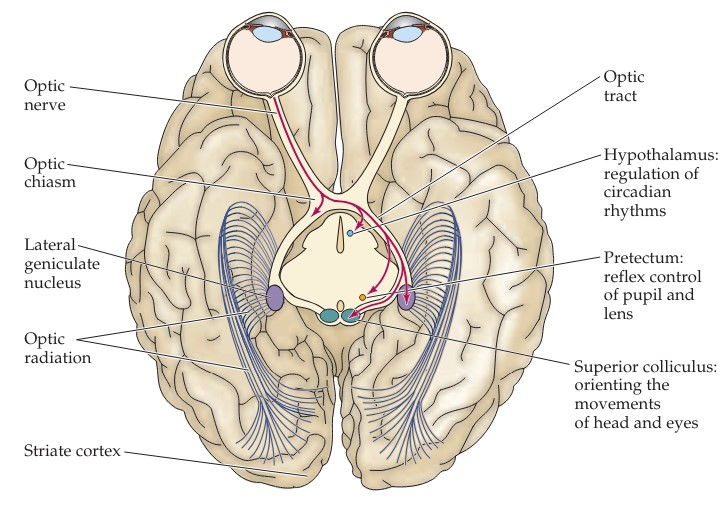
\includegraphics[width=0.7\textwidth]{Visual_Pathway/Central_Visual_Pathway.jpg}
  \caption{詳細視覺路徑圖~\cite{Purves2004Neuroscience3E}}
  \label{fig:Central_Visual_Pathway}
\end{figure}

\subsubsection{視網膜}

外界事物將光反射進入眼睛當中,透過眼珠中的角膜與水晶體等透明的光學介質進行折射最終聚焦於視網膜表面的感光層上形成影像。
在光聚焦於視網膜表層時,視網膜會將光轉換成動作電位並透過視神經傳輸至外膝體,也因此Central Visual Pathway 才會將視網膜視為感知彩色影像的第一個重要部位。

根據《Neuroscience-Exploring the Brain》\cite{bear2016neuroscience}
我們知道視網膜的基礎架構是由五類細胞組成如\cref{fig:RetinaBasic},分別是: 感光細胞、 水平細胞、 無長突細胞、 雙極細胞、 神經節細胞。 感光細胞包含我們常聽到的視錐細胞等負責將輸入的光轉化為動作電位、 雙極細胞負責將會將感光細胞的電位傳送到神經節細胞、
這個傳輸的過程有些則是由水平細胞和無長突細胞協助傳輸,
神經節細胞則負責將最後的資訊傳輸到外膝體之中。

\begin{figure}[H]
  \centering
  \subcaptionbox{
    視網膜基本架構~\cite{bear2016neuroscience}
    \label{fig:RetinaBasic}}
    {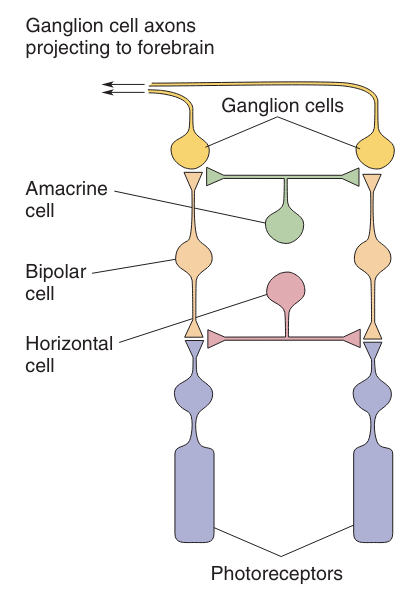
\includegraphics[width=0.5\textwidth]{Visual_Pathway/RetinaBasic.png}
    }
~
  \subcaptionbox{
    視網膜層級架構~\cite{bear2016neuroscience}
    \label{fig:RetinaStructure}
  }
    {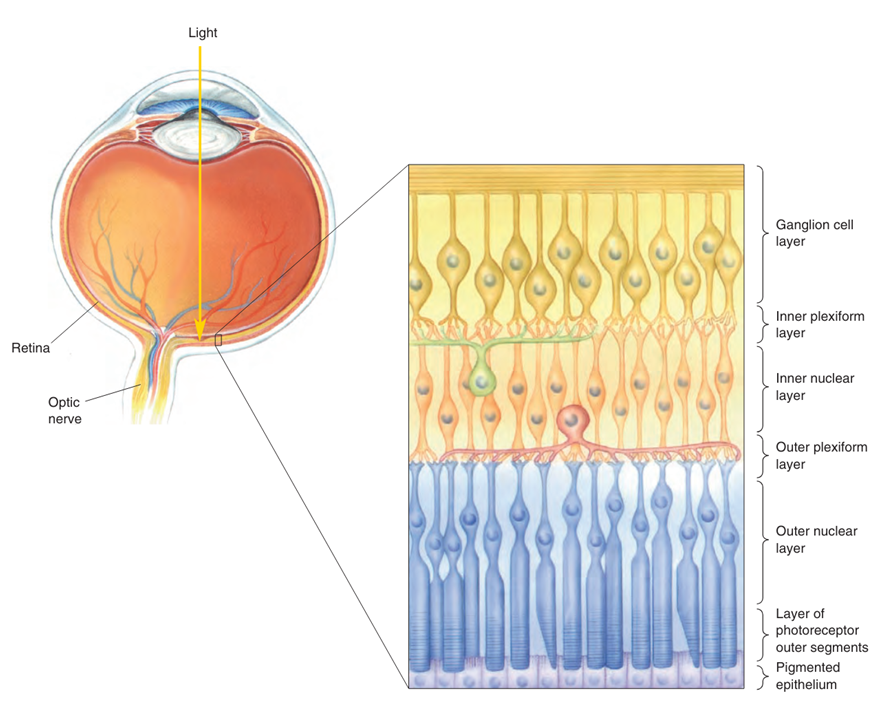
\includegraphics[width=0.9\textwidth]{Visual_Pathway/RetinaStructure.png}
    }
  \caption{視網膜整體架構}
  \label{fig:RetinaTotalStructure}
\end{figure}

上面講的基礎架構只是最基本的情況,事實上視網膜的各類細胞遠比上面要架構要複雜許多,上述的五大類細胞還可以再更細的分為不同功能的變種細胞,由此組成了極度複雜的視網膜層級系統如\cref{fig:RetinaStructure}。
如此複雜的視網膜系統,其功能當然不只負責影像的感知與電位傳輸,事實上
在2013年的\cite{annurev},就已經發現在感光細胞將光轉換為動作電位後會將電位傳輸到層級架構的 Inner Plexiform Layer(IPL)中不同變種的雙極細胞,這些不同變種的雙極細胞對收到的影像資訊進行不同的平行處理,最終輸出影像中不同的方面的要素到神經節細胞,例如: 紅藍綠不同色彩、明暗的變化、影像輪廓等等, 這同時也是本論文在設計彩色影像感知時的核心概念。

\begin{figure}[H]
  \centering
  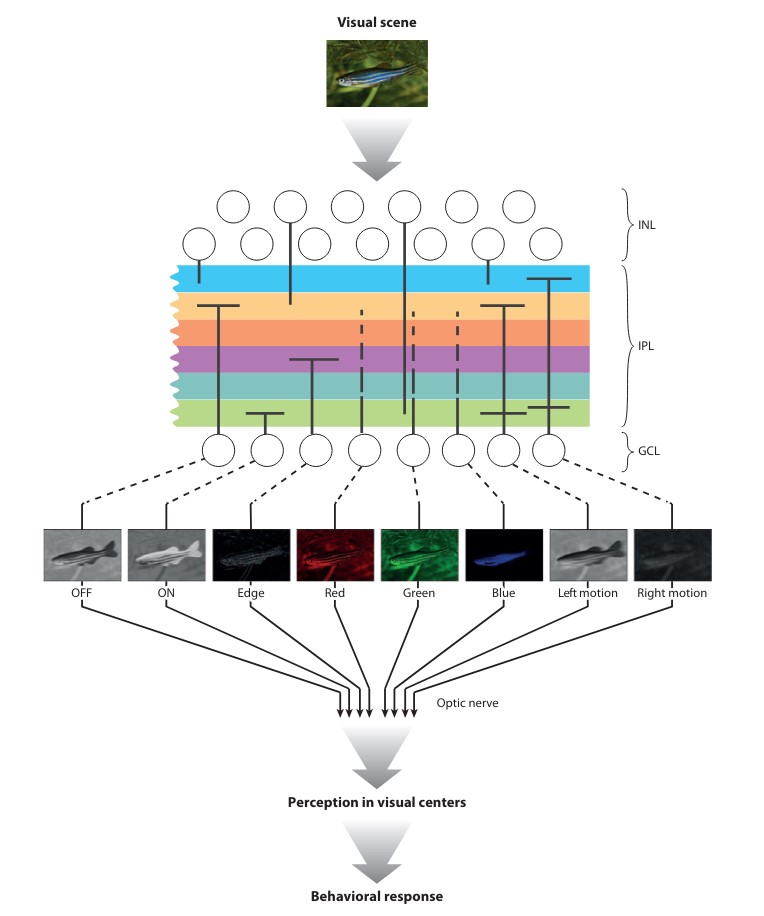
\includegraphics[width=0.7\textwidth]{Visual_Pathway/IPL.jpg}
  \caption{視網膜對影像進行不同的平行處理~\cite{annurev}}
  \label{fig:IPL}
\end{figure}


此外,在Jeff Hawkins的著作\cite{10.5555/993636}和《Principles of Neural Science》\cite{1180370208}中均有提到,
視網膜能接收到的影像資訊不只是上述的空間性資訊,
同時也具有不同時間性的資訊,這代表同樣的影像進入視網膜的型態是會隨時間而改變。
具體而言,眼睛會在每一秒鐘快速移動視線的焦點三到四次(如\cref{fig:Saccade}),
但人類的認知上不會有所感覺,這個行為被稱為 「 眼球跳動 」(Saccade)。
眼球跳動使得同一個影像產生時間上的變化,形成時間性的影像資訊。
這個概念也被運用於本論文的空間位置保留機制中的時間遺忘參數上,
使得影像特徵可以呈現時序上的不同。

\begin{figure}[H]
  \centering
  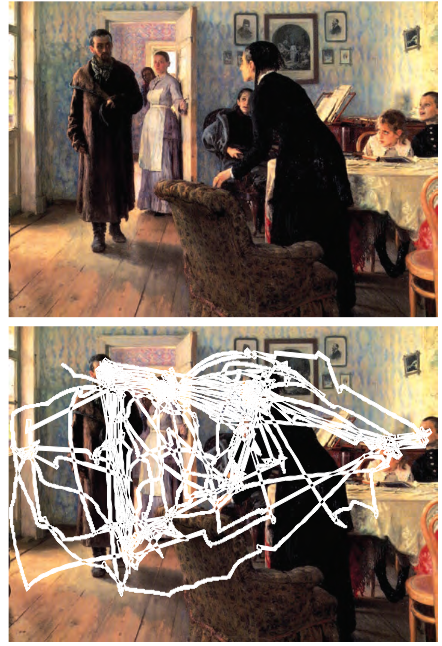
\includegraphics[width=0.7\textwidth]{Visual_Pathway/Saccade.png}
  \caption{眼球跳動示意圖~\cite{annurev}}
  \label{fig:Saccade}
\end{figure}

\subsubsection{外側膝狀體}

外側膝狀體(外膝體)主要負責將視網膜不同的方面資訊(如:色彩、輪廓、運動方向…)傳輸到對應的初級視覺皮質,其中的細胞分層排列,每層分布排列著著不同種類的細胞。
除此之外,外膝體中不同的細胞層也對應著不同視野的半個視網膜形成如 \cref{fig:LGN_Relation}
的對應關係,這也表示視網膜中相鄰區域的同種類的影像資訊在外膝體中很可能在同一個細胞層,
這個性質也保證了外膝體在資訊傳輸的過程可以保留資訊的空間位置資訊。
由於視覺皮層會將影像資訊從初級到高級逐漸進行資訊整合和學習,
因此外膝體的存在可以協助視覺皮層將不同的影像資訊傳輸到對應的視覺皮質層,
這對視覺皮質能夠進行平行處理與整合起到至關重要的作用。

\begin{figure}[H]
  \centering
  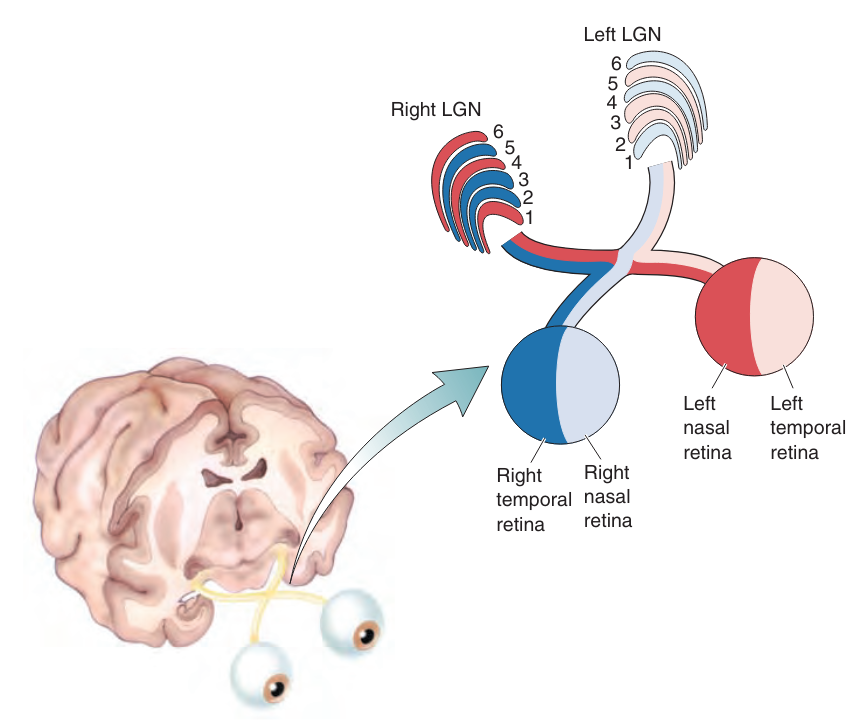
\includegraphics[width=0.7\textwidth]{Visual_Pathway/LGN_relation.png}
  \caption{視網膜與外膝體的對應關係~\cite{bear2016neuroscience}}
  \label{fig:LGN_Relation}
\end{figure}
\pagebreak

\subsubsection{視覺皮層}
皮層可以說是大腦最重要的地方,高級認知功能例如:記憶、思考、感覺等均在此發生。
根據\cite{1180370208}中的說明,人類的大腦中皮質以分層結構存在的,
而視覺皮層又可以分為初級視覺皮層(Primary visual cortex, V1)和紋外皮層(V2、V4、MT層)這四層。
初級視覺皮層負責接收LGN傳輸來的資訊並開始處理顏色、方向、輪廓等視覺資訊,
其餘皮層則負責整合和傳遞資訊給下面的皮層,因此隨著皮層的深入,所得到的視覺資訊也會越來越完整。

\cite{1180370208}提出一種影像資訊處理架構,
示意圖如\cref{fig:ParallelProcess},
其將皮質中的資訊傳輸路徑分成兩類,Ventral Pathway 和 Dorsal Pathway, 
Ventral Pathway 由 V1、V2、V4 組成負責處理影像的色彩、形狀等資訊,
而Dorsal Pathway 由 V1、V2、MT 組成負責處理影像的運動方向的資訊。
但同時也強調這個分類只是一個大致分類,
實際上不同的視覺特徵資訊(如顏色、運動方向等)在皮層中也會相互聯繫,
也就是存在所謂的側向連結,最終才能形成統一的影像感知。

\begin{figure}[H]
  \centering
  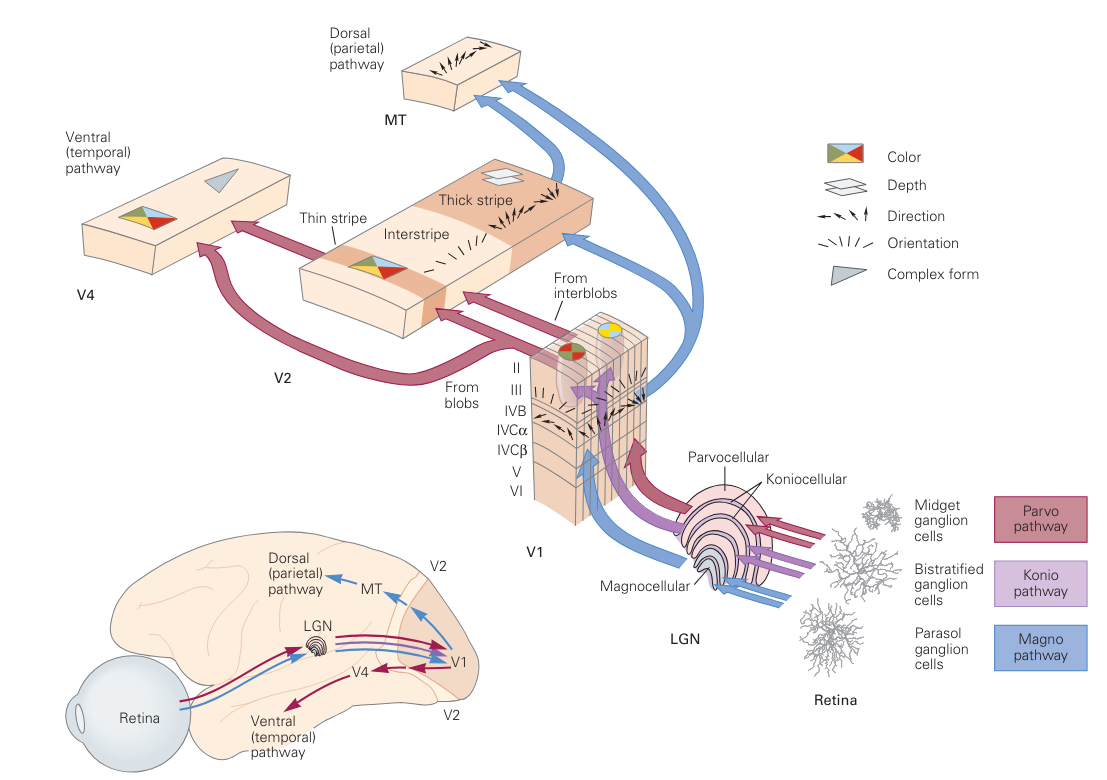
\includegraphics[width=0.8\textwidth]{Visual_Pathway/Parallel_processing_In_contex.png}
  \caption{Visual Pathway的認知過程~\cite{1180370208}}
  \label{fig:ParallelProcess}
\end{figure}

在皮層中,V1 將相同功能的神經束聚在一起形成不同功能的柱狀結構(例如顏色柱、方向柱、線條柱等)
這些柱狀體負責處理各自的視覺資訊並按照固定規則排列成層,
並且將左右眼的柱狀層交錯排列形成一個皮層計算模組(Cortical Computational Module),如\cref{fig:CorticalComputationalModule},重複上百次來覆蓋左右眼看到的所有影像。
這樣設計的目的是希望不管從V1中的任何位置和方向移動都可以漸進的對每塊視野的顏色、輪廓、方向、深度等特徵資訊進行充分的分析。
以上的兩個概念被本論文應用在合併色彩與輪廓特徵與學習綜合特徵中,使我們的模型可以也可以充分學習顏色與輪廓兩個特徵,並隨著層數的深入逐漸組成更完整的影像特徵資訊。

\begin{figure}[H]
  \centering
  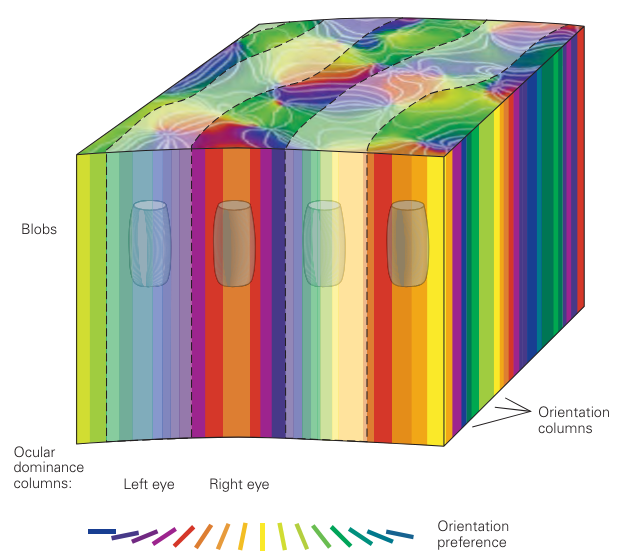
\includegraphics[width=0.7\textwidth]{Visual_Pathway/cortical_computational_module.png}
  \caption{皮層計算模組~\cite{1180370208}}
  \label{fig:CorticalComputationalModule}
\end{figure}
\pagebreak


\subsection{CNN-based Interpretable Model}
CNN-based Interpretable Model(CIM)\cite{YangCNNInterpretable}為 Yang 等人於2023年提出的可解釋性模型,
該模型是模擬大腦視覺皮層的階層架構和影像的時序性關係來解釋深度學習的決策的過程,
目的是希望使模型的決策過程透明化解決黑箱決策的問題。
然而該模型目前只能運用於灰階影像上而無法處理彩色影像的問題,
本論文的目標是基於此模型進行改進,開發出一個更適用於現實彩色影像的新模型。

\subsubsection{模型架構}
該模型採用多層結構,
每層由三個部分組成: 高斯卷積模組、特徵增強模組、空間位置保留合併模組,
整體模型架構如\cref{fig:CIM_arch},
\begin{figure}[H]
  \centering
  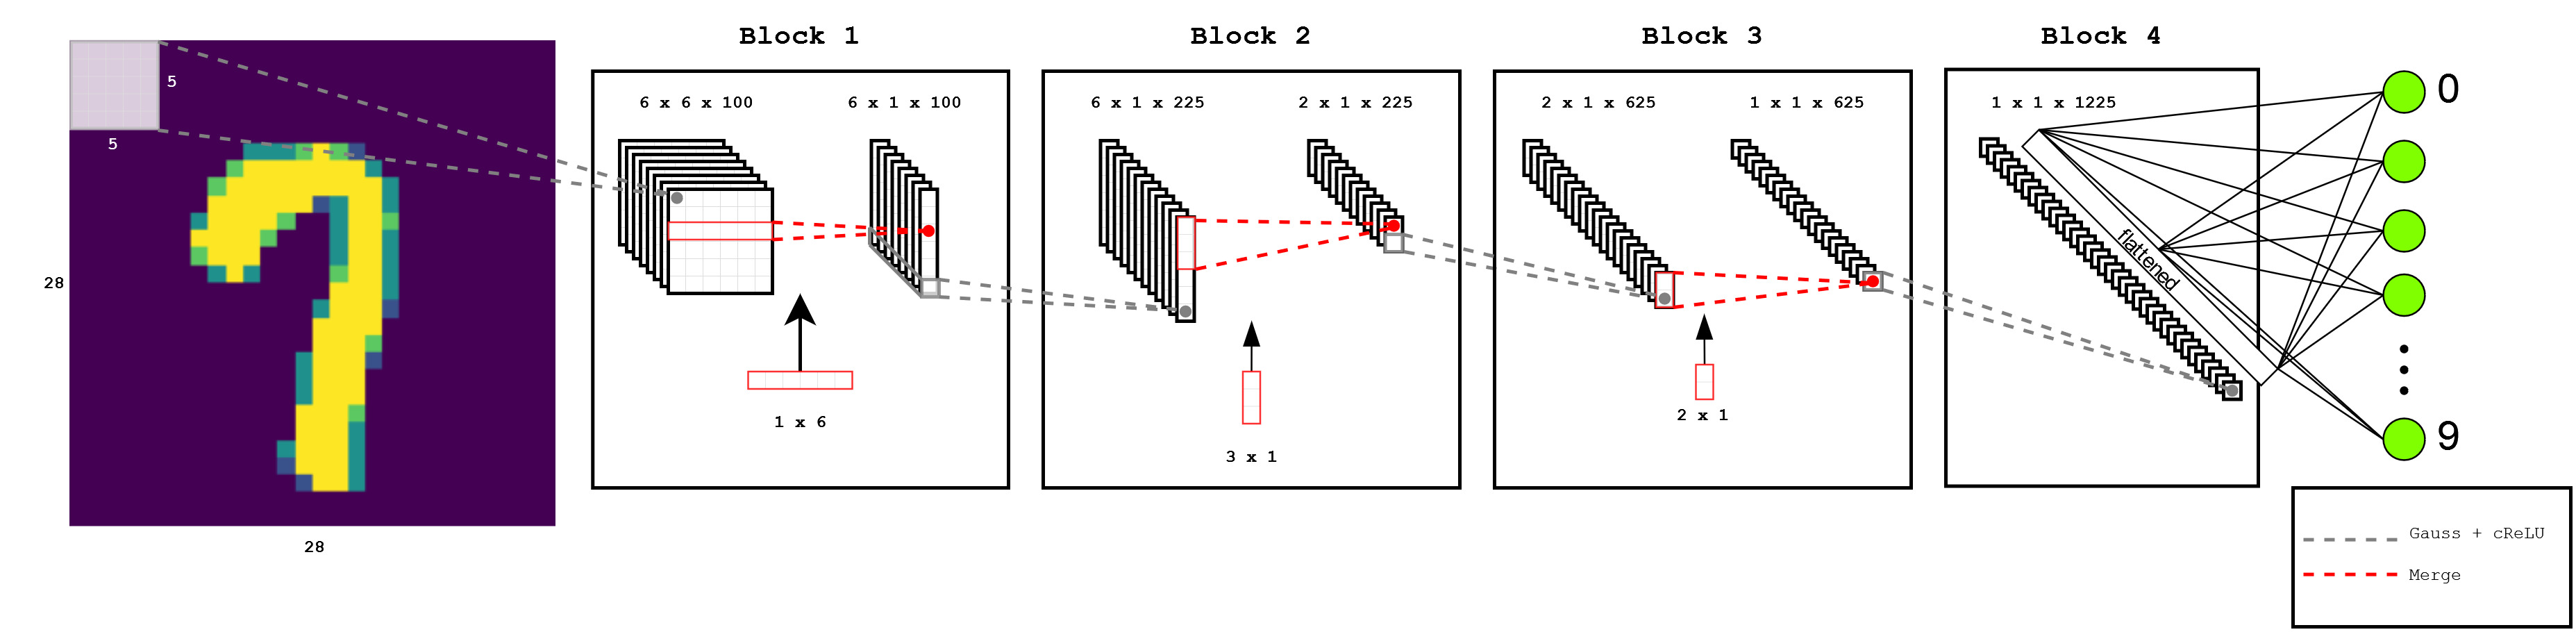
\includegraphics[width=1\textwidth]{CIM/CIM_model_arch.jpg}
  \caption{CIM架構圖~\cite{YangCNNInterpretable}}
  \label{fig:CIM_arch}
\end{figure}


高斯卷積模組使用高斯函數(公式如\cref{eqn:rbf-gaussian-function})取代原始卷積操作中的內積操作來對輸入進行特徵提取,
使得該模組計算的結果具有相似度的意義並且此特性也被運用在後續的可解釋性中。\\
特徵增強模組使用該論文中新提出變形的ReLU函數稱為changed ReLU(簡稱為cReLU)來過濾不重要的特徵使得後續的解釋性可以有更好的發揮。\\
change ReLU的公式如\cref{eq:eq-crelu},$c$為人工取的一個閥值
\begin{equation}
    \label{eq:eq-crelu}
    % f(x) = \max(c, x)
    f(x)= 
    \begin{cases}
        0 & \text{if  $x < c$ }\\
        x & \text{if  $x \geq c$}
    \end{cases}
\end{equation}

空間位置保留合併模組為該論文所提出來的全新機制,
文中他們將一組輸入在經過高斯卷積和特徵增強後產生的輸出稱為$RM$,
而一張影像又擁有多組資訊,從而產生出多張屬於這個影像的$RM$。
使用合併公式\cref{eq:eq-sf}並加入時間遺忘函數(forgetting factor)$\alpha$,來進行合併來模擬特徵資訊在皮層中的時序性特徵資訊與皮層的逐層合併的現象,
從而達到在合併的過程中保留特徵之間的時序關係,
也可讓越後面的層數學習到更完整的特徵資訊。\\
合併公式:\\
$RM_{c}$為合併後的RM,$RM_{k}$為第k張RM,$n$為輸入資訊的數量,$\alpha$為一個可訓練的參
\begin{equation}
    \label{eq:eq-sf}
    RM_{c}=\frac{1}{n} \sum_{k = 0}^{n-1} \alpha^{k} \times RM_{k}  \qquad ,\ where\ n = \textit{H}^{i}_{SF} \times \textit{W}^{i}_{SF}
\end{equation}

\begin{figure}[H]
  \centering
  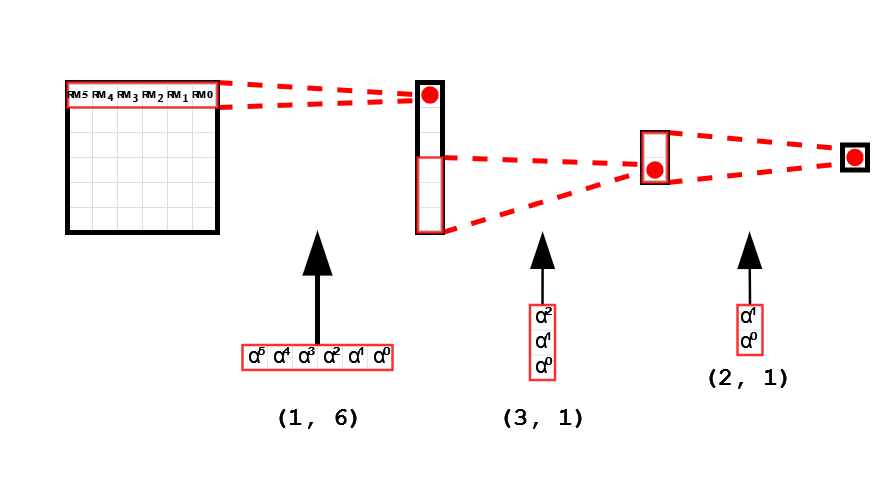
\includegraphics[width=0.7\textwidth]{CIM/CIM_SFM.png}
  \caption{合併方式示意圖~\cite{YangCNNInterpretable}}
  \label{fig:CIM_SFM}
\end{figure}


\subsubsection{可解釋性}
文中將每層的高斯卷積模組的濾波器視為二階矩陣稱為特徵映射圖(Feature Map, $FM$),
一組輸入在每層經過高斯卷積模組和特徵增強模組後的輸出稱為特徵映射響應圖(Response Map, $RM$),
當模型訓練完畢後會讓每個卷積模組中的濾波器對資料集中的所有影像進行反應
並且從所有反應中找到造成最大反應的影像,每個濾波器都會有屬於自己的最大反映影像,
稱為特徵映射圖之對應影像(Corresponding Image, $CI$)
以上的$FM$, $RM$, $CI$ 便是模型提供可解釋性的核心要素,
其關係圖如\cref{fig:one-FM2-RM2-CI2-EXAMPLE}

\begin{figure}[H]
    %\captionsetup[subfigure]{labelformat=empty} % 完全隱藏圖號
    \centering
    \subcaptionbox
        {RM$_{0}$之特徵圖
        \label{fig:one-RM2-EXAMPLE}}
        {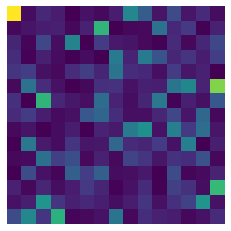
\includegraphics[width=0.33\linewidth]{CIM/fig-one-RM2-EXAMPLE.png}}
    ~
    \subcaptionbox
        {FM$_{0}$之特徵圖
        \label{fig:one-FM2-EXAMPLE}}
        {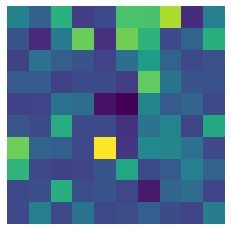
\includegraphics[width=0.33\linewidth]{CIM/fig-one-FM2-EXAMPLE.png}}
    ~
    \subcaptionbox
        {CI$_{0}$之特徵圖
        \label{fig:one-CI2-EXAMPLE}}
        {
\includegraphics[width=0.475\linewidth]{CIM/fig-one-CI2-EXAMPLE.png}}
    \caption{FM-RM-CI\cite{YangCNNInterpretable}}
    \label{fig:one-FM2-RM2-CI2-EXAMPLE}
\end{figure}

在可解釋性的方法上,論文中提出了兩個方法,
第一個方法為特徵圖對應法,
在將一張影像輸入進模型後
第一步視覺化輸入影像中每個區塊在模型中每層的$RM$並找出$RM$中最大反應,
第二步從$RM$最大反應找出造成反應的$FM$,
第三步根據$FM$和$CI$的對應關係,找出該$FM$對應之$CI$,
第四步利用每個區塊的$CI$根據原本的位置組合出輸入影像在模型中被分解的過程
這個方法用於了解模型在經過高斯卷積、特徵增強、空間位置保留合併後所關注的特徵資訊。
範例如\cref{tab:CIM_RMCI_example}

\begin{table}[H]
  \centering
  \begin{tabular}{| c | c | c | c | c |}
    \hline
    原始影像 & RM-CI1 & RM-CI2 & RM-CI3 & RM-CI4 \\
    \hline
    \begin{minipage}[t]{0.18\columnwidth}\centering
\includegraphics[width=0.9\textwidth]{CIM/mnist-16-0-cmp-input.png}\end{minipage} &
    \begin{minipage}[t]{0.18\columnwidth}\centering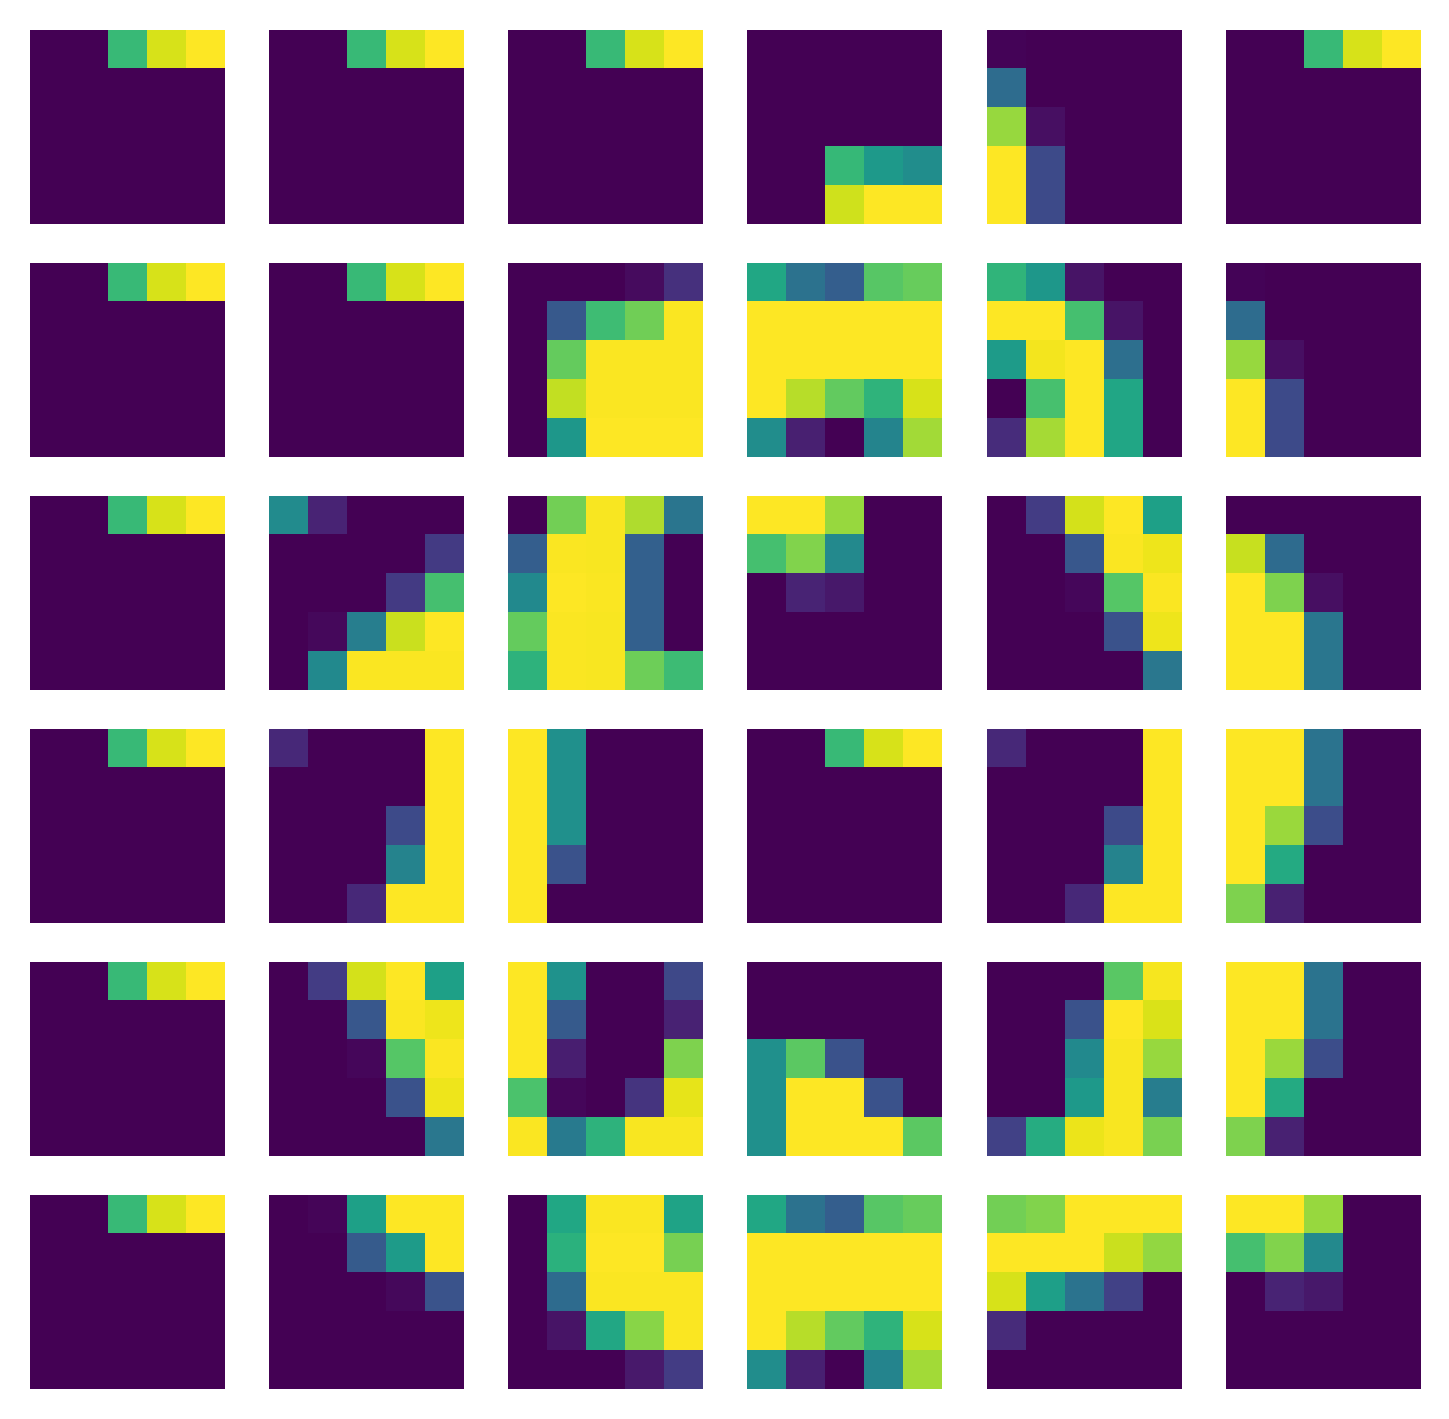
\includegraphics[width=0.9\textwidth]{CIM/mnist-16-0-cmp-rm1-ci-max-1.png}\end{minipage} &
    \begin{minipage}[t]{0.18\columnwidth}\centering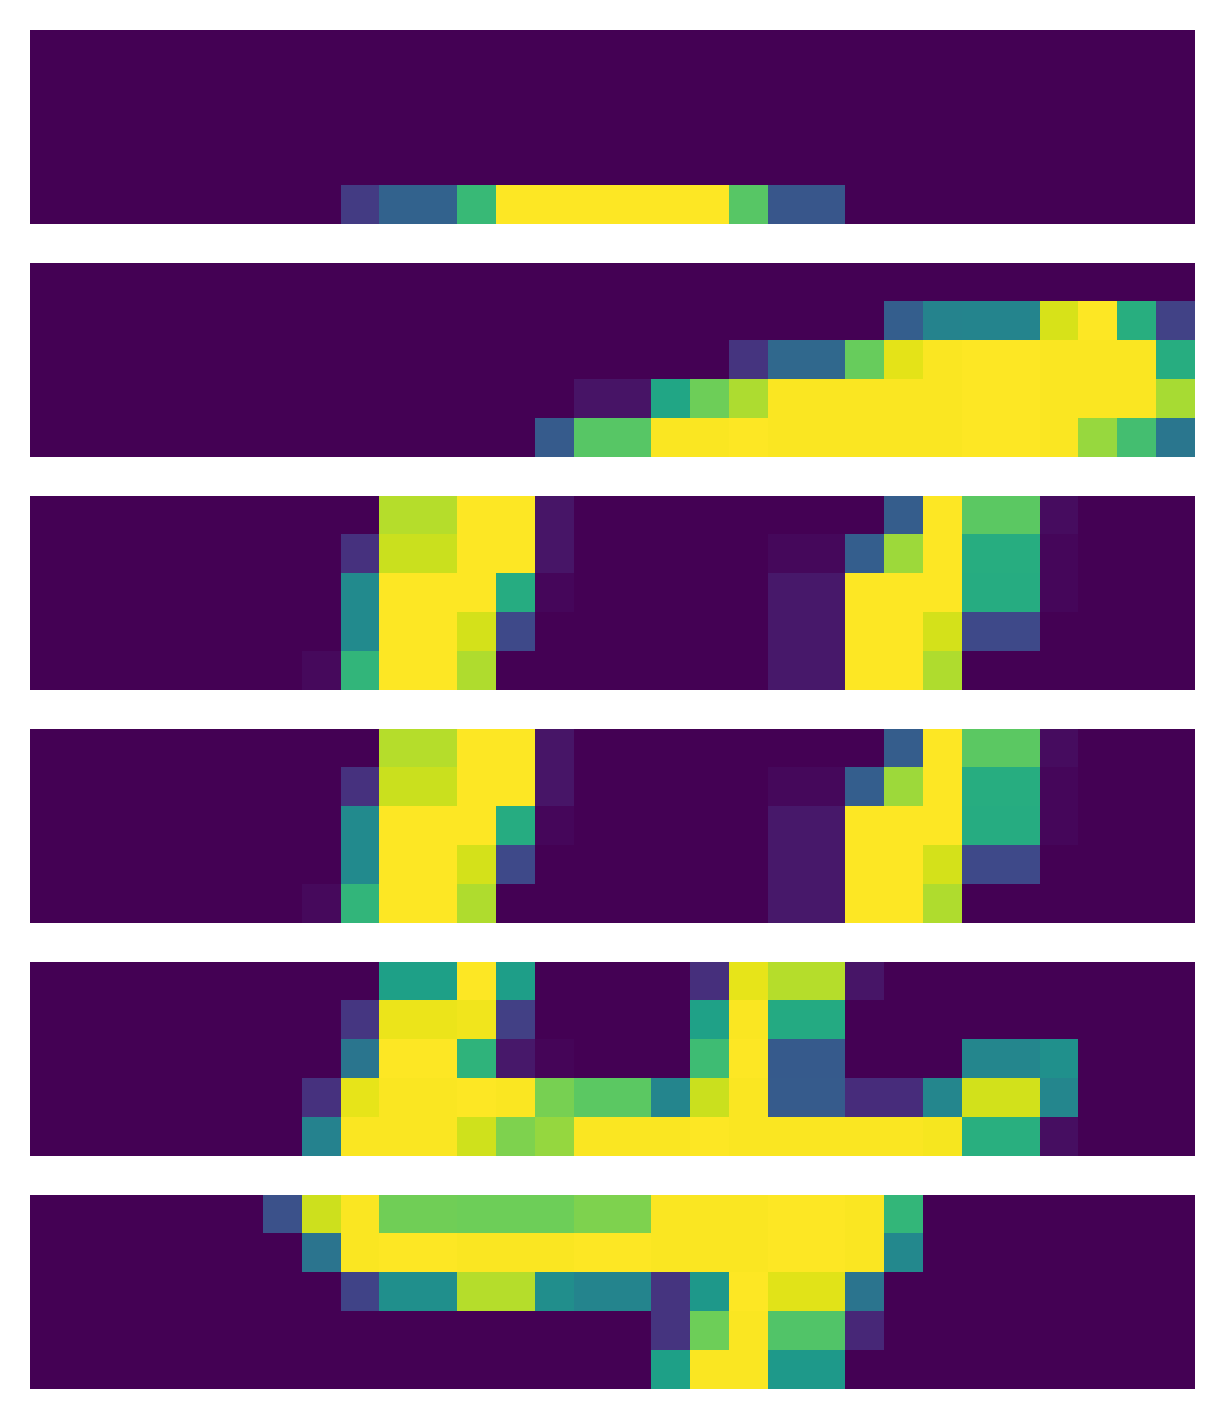
\includegraphics[width=0.9\textwidth]{CIM/mnist-16-0-cmp-rm2-ci-max-1.png}\end{minipage} &
    \begin{minipage}[t]{0.18\columnwidth}\centering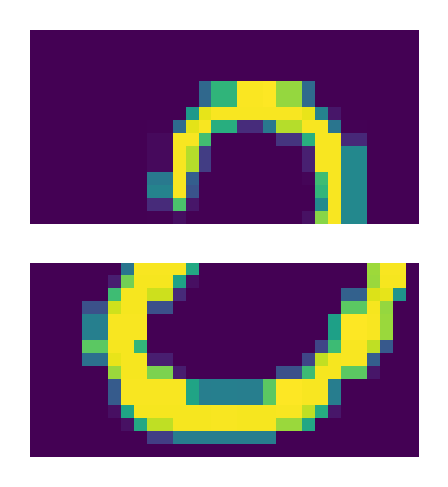
\includegraphics[width=0.9\textwidth]{CIM/mnist-16-0-cmp-rm3-ci-max-1.png}\end{minipage} &
    \begin{minipage}[t]{0.18\columnwidth}\centering
\includegraphics[width=0.9\textwidth]{CIM/mnist-16-0-cmp-rm4-ci-max-1.png}\end{minipage} 
    \\ \hline
    \end{tabular}
    \caption{特徵圖對應法示意圖\cite{YangCNNInterpretable}}
    \label{tab:CIM_RMCI_example}
\end{table}

第二個方法為全連接層權重對應法,
是透過將全連接層的輸入$x$和全連接層的權重$w$的乘積視為$RM$
並且對應之$FM$為最後一個Block的$FM$,透過此$FM$找到$CI$
將全連接層轉成可以理解的資訊。

\section{文獻回顧}

本章節將向讀者介紹可解釋性人工智慧,並回顧可解釋性人中智慧的發展歷程和分類,
協助讀者可以更了解可解釋性人工智慧的現狀與研究方向,


\subsection{可解釋性人工智慧的演進分類}
可解釋性人工智慧(Explainable Artificial Intelligence, XAI)的研究最早可以追蹤到1991年的專家系統時代 W Swartout, C Paris 等人便發覺在金融、醫療,軍事等重要領域中進行的決策中往往需要一個足以支撐結論的合理解釋,
便從此開始對XAI進行研究 \cite{87686}。

XAI從一開始的小眾領域在近些年開始蓬勃發展成活躍的研究領域,
甚至每年都會有各式各樣的 Review Paper 被發表\cite{A2023100230} \cite{10188681},
論其原因應該歸功於近年來人工智慧已被各行各業所應用於分類、物件偵測、資料分析等任務,
隨著人工智慧的普及,在重要領域中XAI的地位和重要性也日益上升。

根據 \cite{Nielsen_2022} 和 \cite{LONGO2024102301} 的研究,
我們將可解釋性人工智慧的研究分為 Ante-hoc 和 Post-hoc 兩大類,
然而這兩類方法均有各自的優缺點,
值得注意的是,在\cite{LONGO2024102301}有介紹到最近有些研究展現出具有解決這兩類缺點的潛力,
但其解釋性仍須更進一步的研究,因此我們將其視為不同於前兩類的第三大類。
以下讓我們介紹這些類別的特性與較為著名的研究。

\subsection{對於 Ante-hoc explainable 模型之研究}
Ante-hoc explainable 模型(\cite{Nielsen_2022}稱為 Interently Interpretable Models),
不同於 Black Box 模型,在模型設計時就會考量可解釋性的需求,
使得模型本身便具備產生解釋性的能力,
其最終目標便是產生一個既準確又可以讓人理解決策過程的深度學習模型。

這類模型最著名的便是機器學習中的Decision Tree(DT)\cite{rokach2016decision},
DT透過一系列的規則去不斷進行抉擇並且可以很容易地被可視化,
使得人們可以容易理解DT的決策邏輯,
並且也經常被用在金融等常運用表格去表示資料的領域\cite{grinsztajn2022tree}。
除此之外也有,例如Nest Generalized Exemplar(NGE)\cite{salzberg1991nearest}、Adaptive-Network-Based Fuzzy Inference System(ANFIS)\cite{256541}、 Collection of High Importance Random Path Snippets(CHIRPS)\cite{hatwell2020chirps}等等模型;

Steven Salzberg 等人於 1991 提出了NGE\cite{salzberg1991nearest}的理論,
該理論將學習到的特徵映射到歐氏距離n維空間(簡稱為En)形成超矩形。
所謂的超矩形是一種幾何學的名詞,可以被視為是在n維空間中的長方體。
NGE便是利用超矩形由於是在n維空間,
因此可以互相與其他的超矩形進行疊加來形成任意深度的和超矩形每個軸可以是任意範圍的兩種特性,透過計算不同的輸入所形成的超矩形之間的距離,來得到高準確度,同時也可以透過幾何解釋模型作出決策的原因。然而這個方法在處理高維資料時面臨複雜性大幅提高的問題,這便是此模型侷限性。

J.-S.R. Jang 等人於1993提出ANFIS模型\cite{256541},其將模糊系統與神經網路進行結合,由神經網路學習模糊規則並藉由模糊引擎來對輸入資料進行判斷。這個模型的本質上維持著模糊系統的架構,因此我們藉由導出模糊規則檢視模型的判斷條件來解釋模型作出的決策。

Hatwell, J., Gaber等人於2020年提出CHIRPS演算法\cite{hatwell2020chirps},該演算法是以Random Forest為基礎,從每棵樹中多數分類的決策路徑並從中找到最常出現的條件,
以這些條件建構出一條條if-then規則,並且分析每個規則的準確度和覆蓋率,提供如果缺少了該規則所造成的影響。該演算法提供之規則在當時與SOTA相同但其覆蓋率更大,並且演算法提供的是人類可以分析理解的規則而不是單純的結果。

以上的研究均在模型本身便具備可解釋性,然而這類模型存在一個問題便是必須再訓練模型前找出有效的特徵提取方法,
模型的可解釋性與準確度都會因為使用不同的特徵提取方法而造成很大的影響。
如何在使用不複雜的特徵提取的同時提高準確度與解釋性也是這類模型的很大的課題。

\subsection{對於 Post-hoc explainable之研究}
Post-hoc explainable method 與 Ante-hoc explainable model最大的差異是,
此種研究所做的並不是開發與"black-box"模型(黑盒模型)相對具可解釋性的"white-box"模型,
而是著重於在模型完成預測之後,對其結果進行解釋。

而\cite{Nielsen_2022}又告訴我們在Post-hoc explainable之下我們可以分成兩類,Local 和 Global,
這兩類的差別在於Local的特點是針對單一筆預測進行解釋,通常採用的辦法是找出關鍵特徵並且解釋該特徵是如何影響到預測,Local之下針對方法又可以分成,以梯度為基礎的方法(Gradient-based)和以局部干擾為基礎的方法(Perturbation-based),
Gradient-based最具代表性的便是Layer-wise Relevance Propagation(LRP)\cite{10.1007/978-3-319-44781-0_8},
而Perturbation-based最具代表性則是Local Interpretable Model-agnostic Explanations(LIME)\cite{10.1145/2939672.2939778}。

Alexander Binder 等人於2016年提出了LRP演算法\cite{10.1007/978-3-319-44781-0_8},該演算法是透過使用模型的倒傳遞演算法,將特定預測類別的分數逐層從輸出逐層傳遞,計算每層的相關性分數,最終回到輸入從而找出關鍵的輸入特徵。此種方法主要的優點便是除了神經網路外,它的原理可以被運用到不同的模型結構之中,但需要選擇合適的分數規則。而LRP的缺點缺點在於由於需要逐層計算每層的相關性分數所以複雜度較高。此外,由於其解釋性是依賴相關性分數的分配與計算,因此選擇合適的分數規則尤為重要。

Ribeiro, Marco Tulio 等人於2016年提出了LIME演算法\cite{10.1145/2939672.2939778},該演算法的核心便是透過為想要解釋預測的輸入影像產生一組干擾樣本,這些干擾將會附加在原始輸入的局部部分形成干擾影像,之後將干擾影像輸入進黑盒模型中進行預測,在著訓練簡單模型(例如:DT、Linear Regression等)使這個簡單的模型能夠接近黑盒模型預測干擾影像的結果,最終透過解釋簡單模型來解釋原始輸入影像。這個演算法的優點在於可以靈活的使用在不同的資料類型和模型架構,然而其缺點在於無法提供模型整體的解釋並且可解釋性依賴於產生的干擾樣本的品質。

Global則是針對模型整體去進行解釋,總結出主要的特徵和判斷條件,呈現模型的判斷邏輯,其中最著名的代表則是SHapley Additive exPlanations(SHAP)\cite{NIPS2017_8a20a862}。

Scott M. Lundberg 與 Su-In LeeSHAP在2017年提出了SHAP這個演算法\cite{NIPS2017_8a20a862}。 SHAP運用了博弈論中Shapley Value的概念,SHAP會為
每個特徵計算其在不同特徵組合的平均貢獻來決定一個Shapley Value來表示特徵的重要性。此外,從研究中也表明每個類別只會有一組唯一的Shapley Value組合。這套方法的優點在於其可以同時提供全域和局部特徵的重要性並且其背後有堅實的博弈論的理論支撐。但其缺點在於實現和計算複雜度較高並且對於不了解博奕論的使用者會難以理解模型呈現出來的Shapley Value。

以上這些方法都是在"black-box"模型預測完後再對其進行解析,
然而這種方法也是存在一些缺點的,他們大多只是表示特定特徵的對於類別的重要性,
但是仍需要人類來解釋其背後所代表的意義,並且也無法解釋特徵是如何影響到類別。

\subsection{近年可解釋性模型趨勢之研究}
\cite{LONGO2024102301}中有寫到近年來也有一些論文展現出解決上面兩種方法缺點的潛力,
其中一種是將注意力的解釋整合到神經網路中,來提高表格類資料的可解釋性的論文\cite{Arik_Pfister_2021},另一種是使用計算論證(Computational Arugmentation)的方式\cite{ijcai2021p600},透過模擬人類推論的過程,
讓模型針對決策過程的每一步提出不同的規則相互論證,
由此來得到決策的每一步過程的正確規則。特別的是這類模型屬於非單調推理(Non-monotonic reasoning),代表其允許有新證據時推翻自己的結論,這樣的方法較為符合人類的常見推理方式。


\subsubsection{Tabnet: Attentive interpretable tabular learning}
\subsubsection{Building more explainable artificial intelligence with argumentation}
XAI的新趨勢使用論證的方式來解釋,特別是計算論證有助於理解理性決策的所有步驟以及在不確定性下進行推理。 \cite{LONGO2024102301}

\end{document}    % 背景知識及文獻回顧
        \documentclass[class=NCU_thesis, crop=false]{standalone}

\begin{document}

\chapter{研究方法}

\section{以卷積神經網路為基礎之新型可解釋性深度學習模型}
\subsection{模型架構}

此章節將介紹本論文所提出的可解釋性模型整體架構與每個部分的功能,並說明資料在模型中的運作方式,模型架構圖如\cref{fig:model_arch_simple}。
整個模型可以分成三個部分,色彩感知區塊、輪廓感知區塊和特徵傳遞區塊。

\fig[1][fig:model_arch_simple][H]{model_arch_simple.png}[模型架構圖][模型架構圖]

\pagebreak

這三種區塊均由不同的卷積模組、響應篩選模組、空間合併模組所組成。
卷積模組利用不同的方式學習與提取輸入的特徵,
響應篩選模組負責過濾不重要的特徵,
空間合併模組則模擬皮層的資訊合併,融合眼球跳動的概念,將輸入的資訊根據空間位置關係進行合併。

色彩感知區塊為單層架構,其架構如\cref{fig:color_arch}
透過彩色卷積模組計算輸入影像不同區塊的色彩與30種基本色彩的相似度去分析輸入影像的色彩分布,
並經過響應篩選模組、空間合併模組,以提取影像中每個區塊的色彩特徵。

\fig[0.5][fig:color_arch][H]{chapter3/color_arch.png}[色彩感知區塊架構圖][色彩感知區塊架構圖]

輪廓感知區塊也為單層架構,
透過將影像進行灰階前處理後,
使用高斯卷積模組、響應篩選模組、空間合併模組,
來提取影像中輪廓和邊緣的特徵。

\fig[0.5][fig:gray_arch][H]{chapter3/gray_arch.png}[輪廓感知區塊架構圖][輪廓感知區塊架構圖]

特徵傳遞區塊為多層架構,
使用了高斯卷積模組、特徵強化模組、空間合併模組
負責處理和學習前面感知區塊所提取的特徵。

\fig[0.5][fig:combine_arch][H]{chapter3/combine_arch.png}[特徵傳遞區塊架構圖][特徵傳遞區塊架構圖]

此外,為了在訓練之後使用者可以對彩色和灰階的可解釋性圖片進行對照,
因此我們對模型加入了一個限制,
限制色彩特徵傳遞區塊和輪廓特徵傳遞區塊的層數和空間合併方式必須相同並且
色彩感知區塊和輪廓感知區塊的高斯卷積模組 Filter 長寬必須相同。

\pagebreak

\subsection{模型符號說明}
	\begin{description}
		\item[]\textit{B}$_{in}$, \textit{H}$_{in}$, \textit{W}$_{in}$:輸入影像之長、寬

		\item[]\textit{FM}:卷積模組之濾波器
		\item[]\textit{RM}:輸入經過卷積模組和響應篩選模組所輸出的結果
		\item[]\textit{CI}:卷積模組之濾波器在資料集的對應影像
		\item[]\textit{SF}$_{i}$:第i層的空間合併模組的濾波器大小(Spatial Filter)
		\item[]\textit{H}$^{SF}_{i}$、\textit{W}$^{SF}_{i}$:第i層的空間合併模組輸出的長、寬

		\item[]\textit{FM}$^{color}_{0}$:色彩感知區塊之彩色卷積模組的\textit{FM}
		\item[]\textit{RM}$^{color}_{0}$:色彩感知區塊之彩色卷積模組的\textit{RM}
		\item[]\textit{CI}$^{color}_{0}$:色彩感知區塊之彩色卷積模組的\textit{FM}的對應影像
		\item[]\textit{H}$^{color}_{Filter}$, {W}$^{color}_{Filter}$: 色彩感知區塊之彩色卷積模組的濾波器長、寬
		\item[]\textit{C}$^{color}_{0}$, {H}$^{color}_{0}$, {W}$^{color}_{0}$:色彩感知區塊之輸出的通道數、長、寬

		\item[]\textit{FM}$^{color}_{i}$:色彩特徵傳遞區塊第i層之高斯卷積模組的\textit{FM}, i = 1$\sim$L
		\item[]\textit{RM}$^{color}_{i}$:色彩特徵傳遞區塊第i層之高斯卷積模組的\textit{RM}, i = 1$\sim$L
		\item[]\textit{CI}$^{color}_{i}$:色彩特徵傳遞區塊第i層之高斯卷積模組的\textit{FM}$_{i}$的對應影像, i = 1$\sim$L
		\item[]\textit{C}$^{color}_{i}$, \textit{H}$^{color}_{i}$, \textit{W}$^{color}_{i}$:色彩特徵傳遞區塊第i層之輸出的通道數、長、寬, i = 1$\sim$L
		
		\item[]\textit{FM}$^{gray}_{0}$:輪廓感知區塊之高斯卷積模組的\textit{FM}
		\item[]\textit{RM}$^{gray}_{0}$:輪廓感知區塊之高斯卷積模組的\textit{RM}
		\item[]\textit{CI}$^{gray}_{0}$:輪廓感知區塊之高斯卷積模組的\textit{FM}$^{gray}_{0}$的對應影像
		\item[]\textit{H}$^{gray}_{Filter}$, {W}$^{gray}_{Filter}$: 輪廓感知區塊之高斯卷積模組的濾波器長、寬
		\item[]\textit{C}$^{gray}_{0}$, \textit{H}$^{gray}_{0}$, {W}$^{gray}_{0}$:輪廓感知區塊之輸出的通道數、長、寬

		\item[]\textit{FM}$^{gray}_{i}$:輪廓特徵傳遞區塊第i層之高斯卷積模組的\textit{FM}, i = 1$\sim$L
		\item[]\textit{RM}$^{gray}_{i}$:輪廓特徵傳遞區塊第i層之高斯卷積模組的\textit{RM}, i = 1$\sim$L
		\item[]\textit{CI}$^{gray}_{i}$:輪廓特徵傳遞區塊第i層之高斯卷積模組的\textit{CI}$_{i}$的對應影像, i = 1$\sim$L
		\item[]\textit{C}$^{gray}_{i}$, \textit{H}$^{color}_{i}$, \textit{W}$^{color}_{i}$:輪廓特徵傳遞區塊第i層之輸出的通道數、長、寬, i = 1$\sim$L
	\end{description}

\subsection{演算法流程}
Step 1:決定整個模型的架構與參數,色彩特徵傳遞區塊與輪廓特徵傳遞區塊之層數均為L

Step 2:對輸入的彩色影像做灰階前處理產生對應的灰階影像

Step 3:將彩色影像(B$_{in}$, 3, H$_{in}$, W$_{in}$)和灰階影像(B$_{in}$, 1, H$_{in}$, W$_{in}$)分別輸入色彩提取層和輪廓提取層。各自的輸出為色彩輸出(B$_{in}$, 30, H$^{color}_{0}$, W$^{color}_{0}$),灰階輸出(B$_{in}$, C${_{gray}}$, H$^{gray}_{0}$, W$^{gray}_{0}$)

Step 4:將色彩輸出和灰階輸出分別輸入進各自的特徵傳遞層進行綜合特徵的學習與合併,
		最終會獲得色彩特徵(B$_{in}$, C$^{color}_{L}$, H$^{color}_{L}$, W$^{color}_{L}$), 灰階特徵(B$_{0}$, C$^{gray}_{L}$, H$^{gray}_{L}$, W$^{gray}_{L}$)

Step 5:將色彩特徵與灰階特徵攤平後concat成為(B$_{in}$, C$^{Linear}_{in}$)並輸入進全連接層學習分類特徵

Step 6:計算 Loss Value 並進行反向傳播


\pagebreak

\section{卷積模組設計與實現}
	% \subsection{卷積模組之實作優化}
	% 	在CIM的高斯卷積模組實作上,
	% 	採用了逐個計算每個 Windows 和濾波器之間的歐氏距離並將結果輸入進高斯函數得出相似度。
	% 	我們改進了這個實作過程,利用了 GPU 的多核優勢,
	% 	將每次卷積的所有位置的 Windows 取出來後平行放入 GPU 的多個核心,
	% 	同時計算這些 Windows 與濾波器的歐氏距離再輸入高斯函數中得出相似度,
	% 	並將這個平行處理方式應用在所有的卷積模組中。
	% 	這樣的實作方式使得整體模型的訓練速度可以大幅提高,
	% 	也完整利用GPU的效能,提升了模型效率。

	\subsection{彩色卷積模組的設計與實現}
		彩色卷積模組為色彩感知區塊的卷積模組,
		該模組主要是透過將濾波器(Filter)設定30個調色基礎顏色的色塊來作為該區塊的權重,
		並使用彩色卷積模組計算出影像中不同區塊之色彩與Filter色彩的響應值。
		以下將針對濾波器之設計、彩色卷積模組,兩個部分進行詳細說明。
		
		\subsubsection{濾波器之設計}
			由於色彩提取區塊的輸入為彩色影像其輸入通道分別為紅、綠、 藍三色的通道,
			我們設定輸出的通道數為固定為30,
			使得濾波器的形狀為 $\left(30 , 3, H^{color}_{Filter},  W^{color}_{Filter} \right)$,
			並將其為 30 種不同RGB色彩的$H^{color}_{Filter} * W^{color}_{Filter}$色塊。

			在30種不同色彩的選擇上,
			我們採用日本色彩研究所於1965年提出的PCCS(Practical Color Co-ordinate System)中的24色相環中(如\cref{fig:PCCS}所示)的顏色,
			再加上紅、綠、藍、黑、白、灰六個基礎色組成。
			由於以上的30色均為基礎顏色(如\cref{fig:30Base}),
			因此我們希望透過計算不同區塊的色彩與這些基礎顏色的響應值來當作區塊的色彩特徵。

			我們選擇使用PCCS體系的24色相環加上六個基礎色,
			是為了驗證使用少量基礎色來初始化濾波器進行彩色卷積是否能夠有效的組合出影像中的色彩特徵。
			在實際應用中,使用者可以自行設定不同的顏色或是其他色相環來進行初始化。

			\fig[0.4][fig:PCCS][H]{chapter3/PCCS.jpg}[PCCS體系的24色色相環\cite{PCCScite}][PCCS體系的24色色相環]

			\fig[0.4][fig:30Base][H]{chapter3/30BaseColor.png}[濾波器設定的基礎30色][濾波器設定的基礎30色]

		\subsubsection{彩色卷積模組}
			\label{chapter:color_convolution}
			在傳統的卷積操作中,
			我們會在輸入影像上使用一個稱為Slide Windows的滑動窗口,
			並且與不同的濾波器進行內積運算來計算輸出,
			這樣的輸出結果只能代表Windows與不同濾波器在平面上的投影而並沒有相似度的意義。
			然而我們在彩色感知區塊的濾波器視為不同的色彩,
			因此我們在計算Windows時會將透過將Windows內的所有像素的RGB值進行加總與平均,
			計算出該Windows的平均RGB值作為該Windows的代表色。
			之後我們計算Windows的代表色與濾波器中不同的顏色的色差,
			並且利用高斯函數取代內積運算將色差轉換為相似度,
			以相似度作為反應強度進行輸出。

			\fig[0.5][fig:colorConvolution][H]{chapter3/color_convolution.png}[彩色卷積示意圖][彩色卷積示意圖]

			在色差的計算上,我們使用由CompuPhase公司提出的一種低成本的加權歐氏距離公式\cite{LABformula}(簡稱LAB Euclidean),
		  	它的權重由RGB中的紅色在色彩中的分量多少而決定。
		  	這種色差計算方法的好處是利用這個公式便可以用兩個顏色的RGB值計算出接近CIE L*a*b(CIE L*u*v)空間中的距離,
		  	同時這套公式也被使用在CompuPhase自己的產品中。
		  	CIE L*a*b是由國際照明委員會提出的色彩空間,
		  	是目前描述人眼可見所有顏色最完整的色彩空間,
		  	因此在CIELAB的距離也會較RGB空間之距離更接近人眼所視。
		  	其公式如\cref{eq:eq-LAB},
		  	其中C$_{1}$代表第一個顏色,
		  	C$_{2}$代表第二個顏色。
		  	\begin{equation}
		    \label{eq:eq-LAB}
		    \begin{split}
		    	\overline{r} & = \frac{C_{1,R} + C_{2,R}}{2} \\
		    	\Delta R & = C_{1,R} - C_{2,R} \\
		    	\Delta G & = C_{1,G} - C_{2,G} \\
		    	\Delta B & = C_{1,B} - C_{2,B} \\
		    	\Delta C & = \sqrt{(2 + \frac{\overline{r}}{256}) * (\Delta R)^2 + 4 * (\Delta G)^2 + (2 + \frac{255 - \overline{r}}{256}) * (\Delta B)^2}
		    \end{split}
			\end{equation}

			\fig[0.5][fig:LabColorSpace][H]{chapter3/Lab_color_space.jpg}[CIE L*a*b 色彩模型][CIE L*a*b 色彩模型]

	\subsection{灰階前處理的設計與實現}
		在輪廓感知區塊中,
		為了使該區塊能夠專注於提取輪廓特徵而不需考慮色彩因素,
		我們會對輸入影像進行前處理。
		首先,我們會將彩色影像轉換為灰階影像,
		轉換公式如\cref{eq:eq-grayscale},
		Gray代表灰階值,R、G、B各代表紅、綠、藍三色通道的值。
		\begin{equation}
		    \label{eq:eq-grayscale}
		    Gray = 0.299 * R + 0.587 * G + 0.114 * B
		\end{equation}
		這種加權方法主要考慮了人眼對於不同色彩的敏感度,
		從而能夠較為完整保留彩色圖像中的細節,
		接著為了消除不同色彩導致的灰度值差異,
		使該區塊能夠專注於輪廓資訊而不考慮色彩資訊,
		我們接者進行了Min-max正規化,
		使每張影像的灰階值統一至[$0, 1$]之間。
		透過上面步驟的前處理,
		我們從而可以確保輪廓感知區塊能夠專注於提取輪廓的特徵。

		\fig[0.7][fig:grayscale][H]{chapter3/grayscale.png}[灰階前處理示意圖][灰階前處理示意圖]

	\subsection{高斯卷積模組的設計與實現}
		\subsubsection{濾波器初始化}
			在這個模型之中,除了色彩感知區塊外,
			其餘區塊的高斯卷積模組的濾波器我們均是使用 Kaiming Uniform \cite{DBLP:journals/corr/HeZR015}的方式初始化濾波器的參數。
			初始化範圍為$[-\sqrt{\frac{6}{\text{fan\_in}}}, \sqrt{\frac{6}{\text{fan\_in}}}]$,
			$\text{fan\_in}$ 為輸入通道數。

			我們在實作中選擇使用 Kaiming Uniform 的原因是因為 Kaiming Uniform 相較於常用的 Uniform 初始化和 Xavier Uniform\cite{pmlr-v9-glorot10a} 初始化多考慮了整流線性單位函數(ReLU)等非線性激活函數的存在,
			Uniform 初始化的方式無法解決隨著神經網路的增加而導致梯度消失的問題,
			Xavier Uniform 為了解決梯度消失問題加入了 Rescale 函數 $\frac{1}{\sqrt{\text{n}}}$但卻只適用於激活函數為線性函數的情況下,
			而 Kaiming Uniform 在解決梯度消失的問題時同時考慮了激活函數為非線性函數的情況
			並在論文\cite{DBLP:journals/corr/HeZR015}中透過實驗證明了Kaiming Uniform 在神經網路在不影響準確度的同時更快收斂。
			由於我們的模型中在響應篩選模組中使用的非線性函數ReLU的變形去進行響應篩選,因此選擇了 Kaiming Uniform 來去進行後面的實驗。

		\subsubsection{高斯卷積模組}
			在高斯卷積模組中,
			流程如下,
			首先分別計算每個濾波器與卷積中的每個Slide Windows的歐氏距離
			其公式如\cref{eq:eq-EulideanDist},
			Windows$_{i}$ 為 Window 中第i個pixel值, 
			Filter$_{i}$為濾波器中第i個pixel值,
			C$_{in}$為輸入的channel數,
			Filter$_{H}$, Filter$_{W}$ 為卷積的濾波器大小,
			dist為該濾波器與Window的歐氏距離。
			在得到每個濾波器與每個Windows之間的歐氏距離後,
			再將其輸入高斯函數計算出每個濾波器每個Windows之間的相似度,
			並將其作為響應值進行輸出。

			\begin{equation}
			    \label{eq:eq-EulideanDist}
			    dist = \sqrt{\sum_{i = 1}^{K} (Windows_{i} - Filter_{i})^{2}} \quad where \; K = Filter_{H} * Filter_{W} * C_{in}
			\end{equation}

				我們在此利用高斯函數取代內積的原因在於高斯函數是以距離為基礎的函數,
			其計算結果能夠反映出距離的意義並且表達向量間的相似度,
			而相似度在後續的解釋性表現中幫助我們更好的理解模型的可解釋性圖片產生之原因。\\
			高斯函數(Gaussian function):\\
			  $x$ 為輸入值、$m$ 為中心點、$\sigma$ 為寬度參數
			  \begin{equation}
			      \label{eqn:rbf-gaussian-function}
			      \phi (x) = \exp \left( -\frac{dist^2}{2\sigma ^2} \right) 
			  \end{equation}

\pagebreak

\section{FM、 RM的定義}
	特徵映射圖(FM)為將卷積模組的濾波器提取出來的結果,
	由於模型在高斯卷積模組為計算輸入濾波器與相似度,
	因此FM可以被視為模型學習到了輸入影像中的何種特徵。

	\fig[0.7][fig:FM_picture][H]{chapter3/FM.png}[FM示意圖][FM示意圖]

	特徵映射響應圖(RM)為當輸入進入卷積模組後所得到的輸出,
	其代表的是輸入區域對於該高斯卷積模組的濾波器的相似度,
	也被視為輸入對該高斯卷機模組所有的濾波器的反應強度。
	同一層、不同位置的RM數值為輸入影像的不同位置對於某個濾波器的反應,
	不同層、同一位置的RM數值為輸入影像的同一位置對於不同濾波器的反應。

	\fig[0.7][fig:RM_picture][H]{chapter3/RM-example.png}[RM示意圖][RM示意圖]

\pagebreak

\section{響應篩選模組之設計}
	% 在響應篩選模組中,
	% CIM 使用了自行設計的增強特徵的整流線性單位函數(changed ReLU, 簡稱cReLU),
	% 希望透過閥值過濾不重要的特徵,其公式如\cref{eq:eq-crelu}所示,
	
	% 作為閥值的 $c$ 值需要透過觀察資料集在高斯卷積模組的輸出來設定具體不同的$c$的數值來適應不同的資料集。
	% 然而一旦閥值設定過小則會削弱響應篩選的效果,
	% 閥值設定過大則會將大部分的特徵都歸零導致無法學習出有效特徵,
	% 因此如何設定 $c$ 則成為一個非常困難的問題,並且每次更換資料集都必須面對這個問題。

	% 為了解決閥值設定的問題,
	% 我們對cReLU的公式進行改善,
	
	響應篩選模組的主要目的是過濾卷積後響應較弱的值,
	保留響應較強的值,
	從而在後續產生可解釋性圖片時能有更好的呈現效果。

	我們將輸入的所有RM的響應值總個數$N_{RM}$,
	並設定一個希望保留的RM的百分比參數 $p\%$,
	這代表我們希望保留所有RM中響應值最大的前$p\%$的元素。
	接著從RM中取出第 $p\% * N_{RM}$  個最大的元素稱之為$P_{RM}$,
	並且將所有小於$P_{RM}$的數值歸零,
	篩選公式如\cref{eq:eq-cReLUPercent}。
	此公式代表的意義為保留響應值前$p\%$最大的值並刪除其餘響應值較弱的值。
	
	篩選公式為\\
	\begin{equation}
	    \label{eq:eq-cReLUPercent}
	    f(x)= 
	    \begin{cases}
	        0 & \text{if  $x < P_{RM}$ }\\
	        x & \text{if  $x \geq P_{RM}$}
	    \end{cases} \quad where \; P_{RM} = RM\left[ p\% * N_{RM} \right]
	\end{equation}

	我們選擇使用 cReLU 函數而非傳統的 ReLU、Sigmoid 或 Leaky ReLU 函數,
	原因在於傳統的 ReLU、Sigmoid 和 Leaky ReLU 均為全域性函數,
	主要針對負數部分進行篩選或減弱。
	由於我們的響應值域在 [0, max(RM)] 範圍內,
	使用 ReLU、Sigmoid 或 Leaky ReLU 函數將無法去除過小的響應值。
	然而,cReLU 函數可以根據輸入範圍進行局部篩選,
	從而有效地去除過小的響應值,只保留響應值較大的部分,提升了模型的表現。

\pagebreak

\section{空間合併模組之設計}
	% 在空間合併模組上,
	% CIM為了保留 $RM$ 之間的空間位置關係簡化了眼球跳動的方式,
	% 加入了一個可訓練的時間遺忘函數 $\alpha$ 進入合併公式,其公式如\cref{eq:eq-sf}。
		
	% 這樣會導致越早被看到(時間越早)的數值需要乘上的 $\alpha^{k}$ 的 $k$ 值越大,
	% 在合併時的加權也就越小。
	% 儘管這種做法確實可以使輸出值呈現出空間上的關係,
	% 然而當我們需要合併的$RM_{k}$越多時,
	% 隨著$k$ 值越來越大,$\alpha^{k}$會快速變小。
	% 這樣便造成當我們將數值乘上過小的的$\alpha^{k}$後,
	% 便會變得這個數值便會在最終合併結果中變得無足輕重。
	% 對於大小較大的影像而言這種方法是有問題的,
	% 這會使得影像逐漸喪失一部分特徵。

	% 此外,
	% 在 CIM 的空間合併模組中為了方便輸出可視化圖片
	% 在實作上對輸入進行了維度轉換,
	% 將最後一維 Reshape 成一個二維矩陣,
	% 稱為特徵響應圖(RM)(其操作如\cref{fig:RM_picture}),
	% 然後乘上$\alpha$值進行合併。
	% 然而,我們認為此步驟會造成兩個問題:
	% 首先,CIM原本在第一層高斯卷積後的高斯卷積模組都只是做(1,1)的卷積操作,
	% 但是加入了這個步驟就會導致後續的高斯卷積模組的濾波器大小改變,容易引起閱讀者的誤解;
	% 其次,這個步驟並不會增加準確度或是增加效能,反而是多一些所轉置與Reshape所需要的時間。
	% 基於以上原因我們決定將此步驟捨棄。
	% 在空間合併模組前不再進行維度轉換和Reshape,
	% 並將輸入重新命名為GFR(Gaussian Feature Response),
	% 以區別於原來的RM。
	% 由於我們在空間合併模組前並沒有進行維度轉換和Reshape,
	% 因此公式的輸入使用RM的代稱已不再準確,
	% 所以我們將沒有進行轉換的空間合併模組輸入重新命名為GFR(Gaussian Feature Response)
	% 來與原來的RM做區分。

	在空間合併模組中,
	我們模擬皮層的層狀合併架構(\cref{fig:CorticalHierarchy})和眼球跳動的概念(\cref{fig:Saccade}),
	運用不同的加權參數值模擬眼球跳動的順序,
	將RM根據其空間位置關係對應到不同的加權參數值後進行合併,
	使得下一層卷積模組能夠在考慮特徵空間位置的前提下學習更大範圍的特徵。

	其步驟如下:
	一組輸入資訊經過卷積模組和響應篩選模組後會產生一個RM三維矩陣,
	一張輸入影像為多組輸入資訊的集合,因此產生多個RM矩陣,
	並且將這些RM根據 $SF_{i}$ 透過\cref{eq:eq-sf-update}進行合併,
	產生新的累積特徵響應圖(ARM)並輸入到下一層。

	為了保留RM之間的空間關係,
	我們先從[ $0.9 \sim 0.99$ ]之間進行等距採樣由小到大得到 $k$ 個值,
	將其稱為$\beta_{k}$。
	k 越小代表越早被眼球注視,k越大表示越晚被眼球注視,
	並按照RM合併的順序,
	將RM和$\beta_{k}$相乘並加總。
	其合併公式如\cref{eq:eq-sf-update},
	$ARM_{c}$為合併後的ARM,
	$RM_{k}$為第k個RM,
	$\beta_{k}$為從[$0.9 \sim 0.99$]之間取出的第$k$個值,
	${H}_{i}^{SF}$、${W}_{i}^{SF}$為第i層空間合併模組輸出的長和寬:\\
		\begin{equation}
		    \label{eq:eq-sf-update}
		    ARM_{c}=\frac{1}{n} \sum_{k = 0}^{n-1} \beta_{k} \times RM_{k}  \quad where \; n = \textit{H}^{i}_{SF} \times \textit{W}^{i}_{SF}
		\end{equation}

	% 得到 $k$ 個值代替 $\alpha^{k}$ 按照時序順序去乘以GBF ,
	% 我們將第 $k$ 個 $GFR$ 所對應的 $\alpha$ 稱為 $\beta_{k}$,
	% 如此便可以改善當需要合併的 $RM$ 數量過多時 $\alpha^{k}$ 過小的問題,
	% 同時也保留了CIM當初設計時希望保留的輸入之間的對應空間關係。\\
	
	
	RM的優化後的合併示意圖如\cref{fig:SFN_update}。
	\fig[0.5][fig:SFN_update][H]{chapter3/SFM_update.png}[優化後空間位置保留機制示意圖][優化後空間位置保留機制]


\pagebreak
\section{可解釋性} 
本研究以RM-CI做為解析模型的決策過程的基礎,
使得模型的決策過程可以被視覺化出來,
讓使用者了解模型關注的特徵資訊與決策背後的邏輯關係。

	\subsection{CI的意義}
	\label{section:InterablePicture}

	特徵映射圖之對應影像(CI)為記錄資料集中所有影像對特定濾波器的反應,
	從中選出與該濾波器有最大的反應的影像,
	並該影像視為該濾波器的對應影像。
	會需要CI的原因在於除了顏色感知區塊和輪廓感知區塊之外,
	後續的特徵傳遞區塊的輸入均為前一區塊所計算出來的相似度,
	人類已無法去解讀出FM的意義。
	因此我們需要透過CI來找出該濾波器與何種影像最相似,
	幫助使用者理解FM代表的特徵長相。
	每一個區塊每一層的高斯卷積模組的濾波器都會有屬於自己的對應CI影像。
	產生CI的流程如下:
	\begin{itemize}
		\item [1]
		決定要產生CI的目標濾波器
		\item [2]
		將訓練資料集所有影像按照感知區塊之卷積模組的Filter大小進行分割
		\item [3]
		將所有資料集影像輸入進模型,並且記錄目標濾波器所有的輸出
		\item [4]
		選出目標濾波器所有的輸出的最大值,並且找出該最大值的位置
		\item [5]
		選擇該位置在分割影像中的對應小圖
		\item [6]
		分析在目標濾波器所屬的高斯模組前是否有經過空間合併模組。\\
		如果有,則將分割影像按照空間合併範圍進行合併作為目標濾波器的對應CI
	\end{itemize}


	\begin{figure}[H]
	\centering
	\label{fig:CI_generator_0}
	\captionsetup{justification=centering}
	\caption{色彩感知區塊與輪廓感知區塊的CI產生流程示意圖 \\ 以輪廓感知區塊的高斯卷積模組為例}
	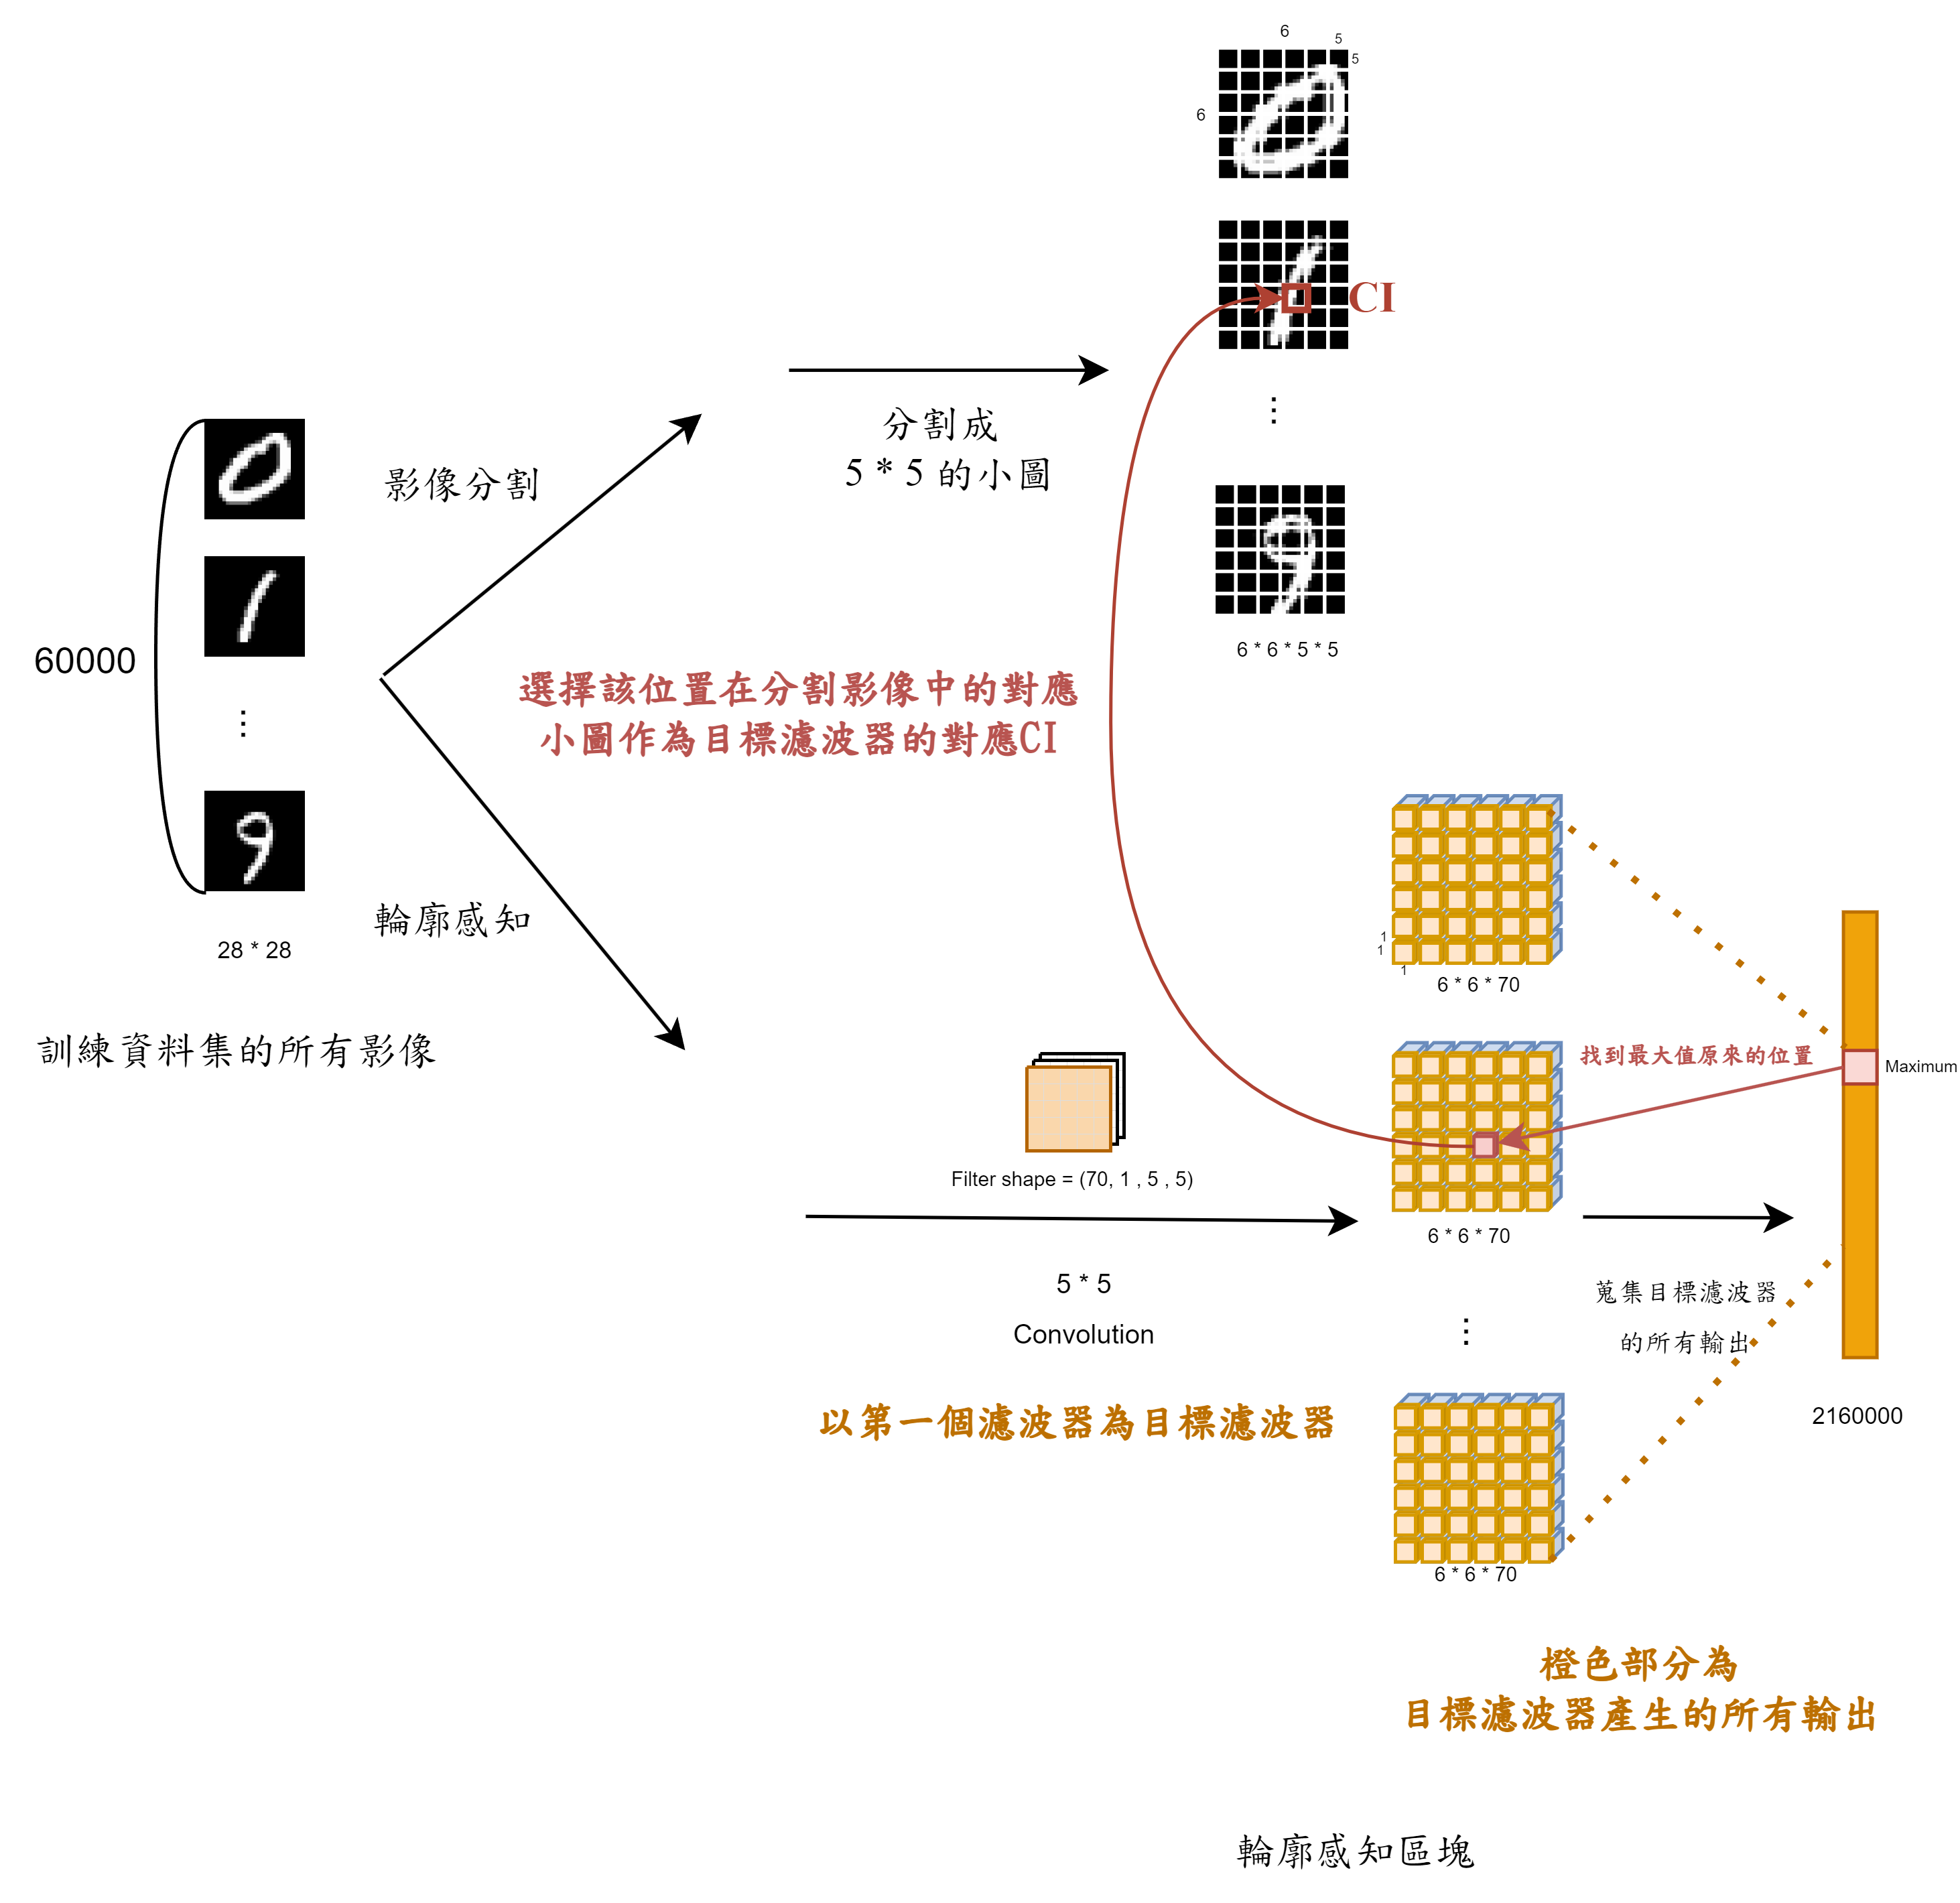
\includegraphics[width=1\textwidth]{chapter3/CI_genenrator_0.png}
	\end{figure}

	\fig[1][fig:CI_generator_1][H]{chapter3/CI_genenrator_1.png}[特徵傳遞區塊之CI產生流程示意圖 \\
	以輪廓特徵傳遞區塊的第一層為例][特徵傳遞區塊之CI產生流程示意圖]

	\begin{figure}[H]
    \centering
    \subcaptionbox
        {
        \label{fig:CI_color_0}}
        {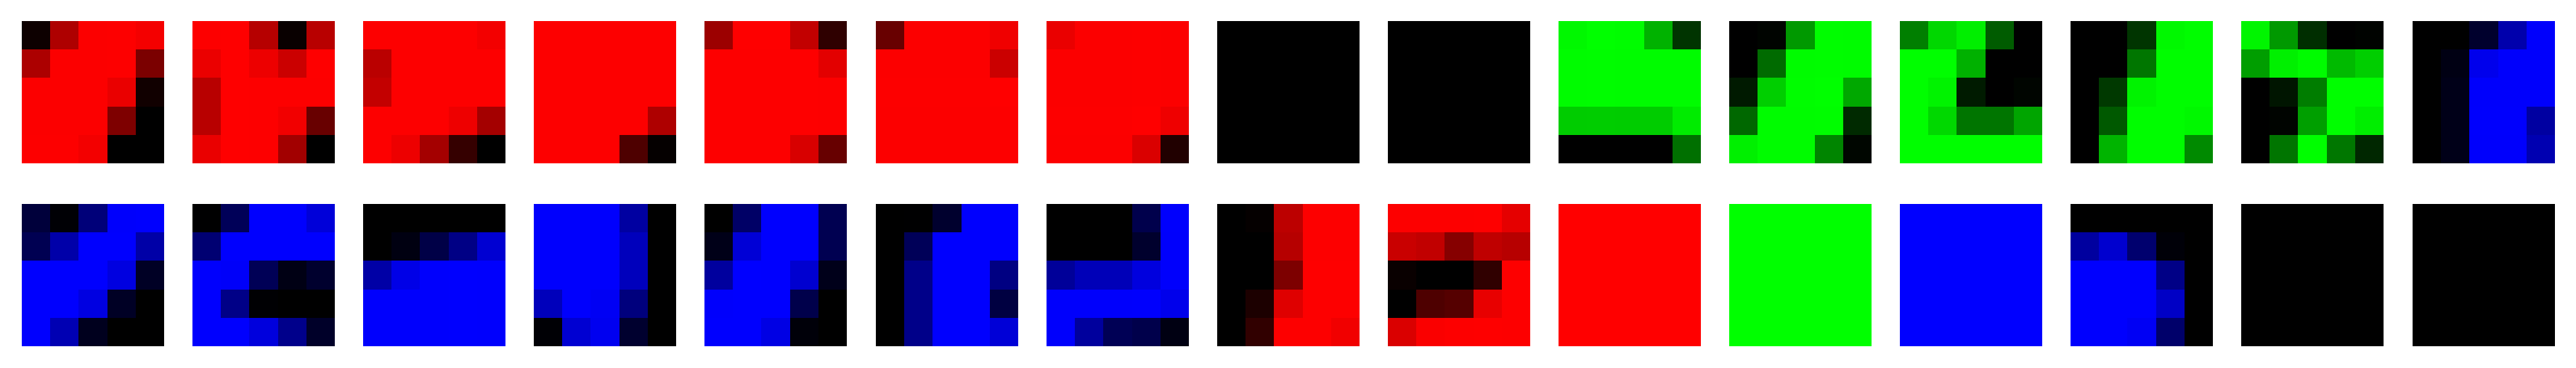
\includegraphics[width=0.3\linewidth]{chapter3/CIs/CIs_RGB_convs_0.png}}
    ~
    \subcaptionbox
        {
        \label{fig:CI_color_1}}
        {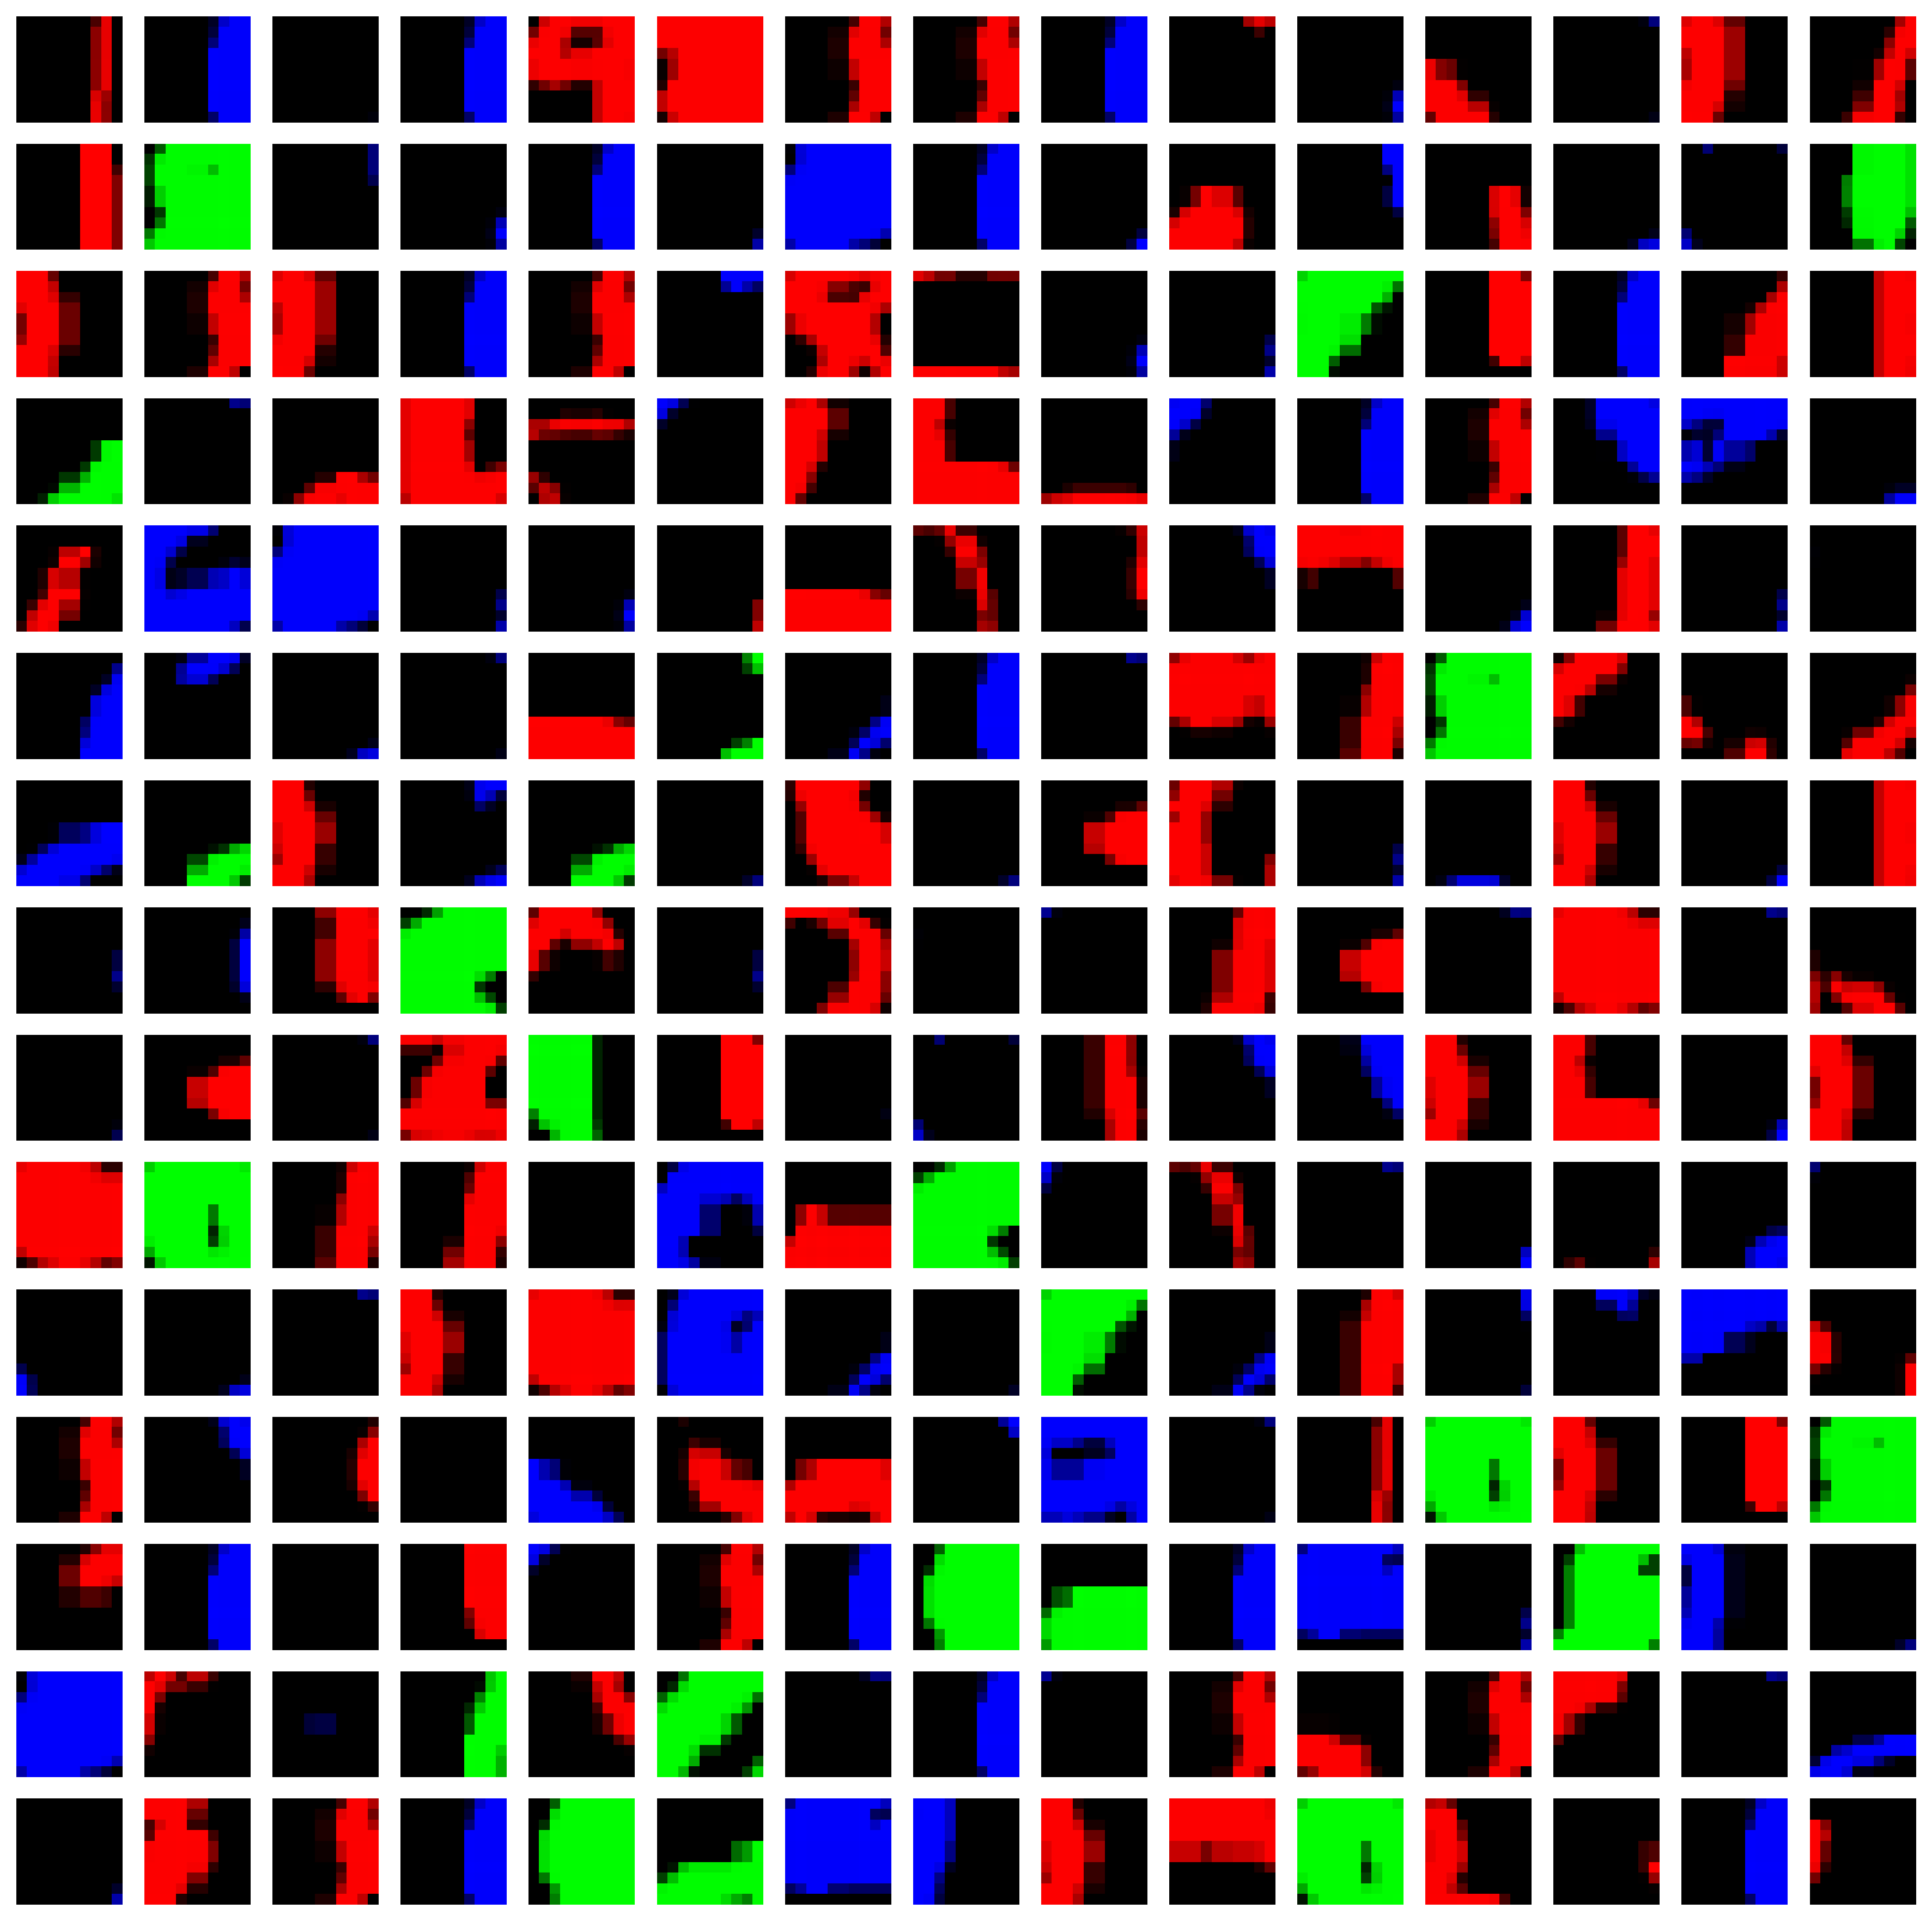
\includegraphics[width=0.3\linewidth]{chapter3/CIs/CIs_RGB_convs_1.png}}
    ~
    \subcaptionbox
        {
        \label{fig:CI_color_2}}
        {\includegraphics[width=0.3\linewidth]{chapter3/CIs/CIs_RGB_convs_2.png}}

     \subcaptionbox
        {
        \label{fig:CI_gray_0}}
        {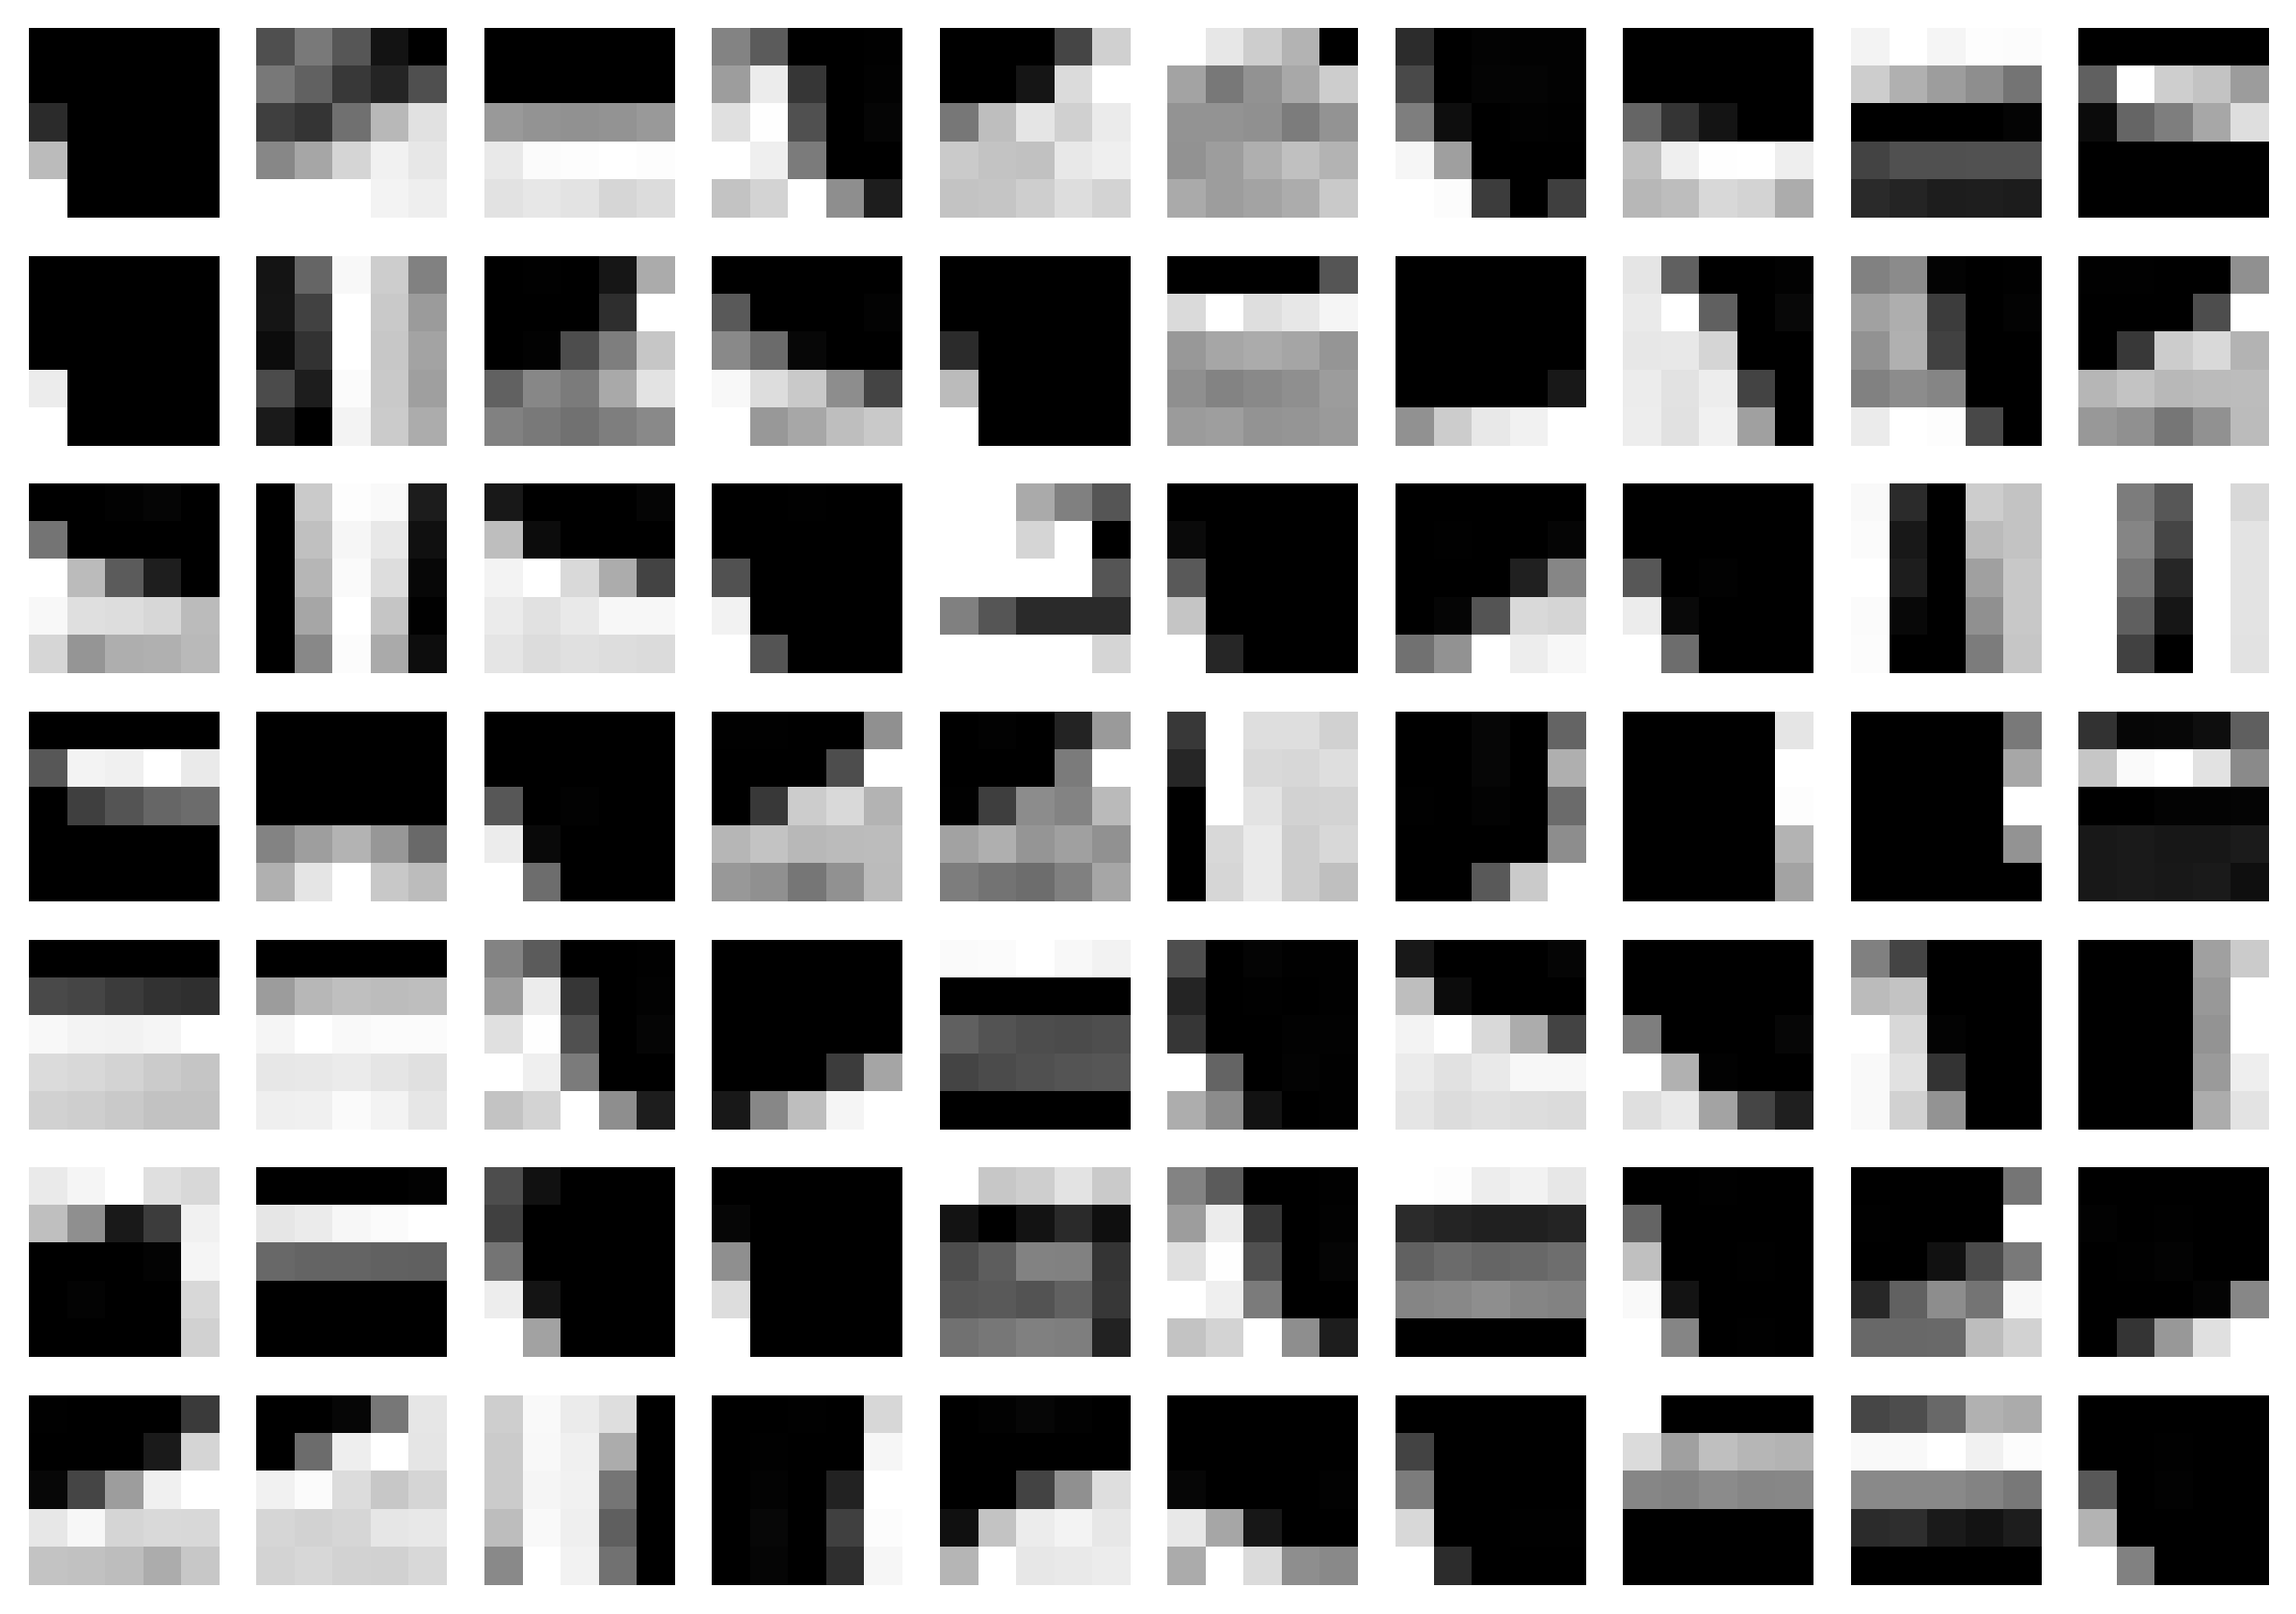
\includegraphics[width=0.3\linewidth]{chapter3/CIs/CIs_Gray_convs_0.png}}
    ~
    \subcaptionbox
        {
        \label{fig:CI_gray_1}}
        {
\includegraphics[width=0.3\linewidth]{chapter3/CIs/CIs_Gray_convs_1.png}}
    ~
    \subcaptionbox
        {
        \label{fig:CI_gray_2}}
        {\includegraphics[width=0.3\linewidth]{chapter3/CIs/CIs_Gray_convs_2.png}}
    \caption{架構中各層的CI範例 (a) $CI^{color}_0$;(b) $CI^{color}_1$;(c) $CI^{color}_2$;(d) $CI^{gray}_0$; (e) $CI^{gray}_1$;(f) $CI^{gray}_2$}
    \label{fig:CIs}
	\end{figure}

	\pagebreak
	\subsection{色彩感知區塊之視覺化}
	在色彩感知區塊濾波器本身即可被視為 \textit{C}$^{color}_{0}$ 個不同RGB顏色,
	並且這個特性導致FM不會學習到輪廓的特徵。
	然而由於CI是由資料集中影像的部分區塊組成,
	因此FM對應的CI的影像反而卻同時存在顏色和輪廓,
	這會導致最後組合起來導致CI容易出現顏色相似,
	但輪廓與輸入影像完全不同的情況,看起來會十分怪異。
	為了解決這個問題,
	我們會取每個CI的平均色彩作為該CI的代表色,
	我們接著會將CI的代表色擴張為和原始CI相同大小色塊,
	並且使用這些色塊代替原本的CI進行呈現,
	從而更好的反應FM學習到的色彩特徵。

	總結色彩感知區塊產生可解釋性圖片的流程如下:
	\begin{itemize}
		\item [1]
		輸入影像後,找出色彩感應區塊的RM
		\item [2]
		從RM中找出每個RM的最大響應值
		\item [3]
		根據RM的最大響應找出造成響應的濾波器對應的CI
		\item [4]
		找出對應CI的代表色並擴張成與原始CI相同大小的色塊
		\item [5]
		利用色塊組出代表輸入影像各個區域在該層反應最大的濾波器感知到的特徵的影像(RM-CI-Color-0)
	\end{itemize}

	\fig[0.6][fig:RMCI_Color_generator][H]{chapter3/RMCI_Color_generator.png}[色彩感知區塊產生RM-CI流程圖][色彩感知區塊產生RM-CI流程圖]

	\pagebreak

	\subsection{色彩特徵傳遞區塊之視覺化}
	在色彩特徵區塊上,
	由於經過空間合併模組的特徵合併,
	因此該區塊所學到的是比色彩感知區塊更加完整的特徵。
	為了準確地呈現FM對應的CI的不同的顏色與位置,
	我們採用以下的方法進行處理:\\
	首先,我們找到輸入影像在該區塊的高斯卷積模組對應的CI。
	接者,將這些CI切成與$CI_{color}$相同大小的小圖,
	然後,對這些小圖分別取平均顏色並將這些平均顏色擴張為和$CI_{color}$相同大小的色塊,
	用這些色塊代替原本的CI按照對應位置組成RM-CI影像。
	再加入了分割這個步驟後,每個CI都能反映出不同部分對應的顏色和位置,
	從而更好的呈現CI的顏色分布。

	\fig[0.7][fig:Color_CI][H]{chapter3/Color_CI.png}[色彩特徵傳遞區塊產生CI示意圖][色彩特徵傳遞區塊產生CI示意圖]

	總結色彩特徵傳遞區塊產生可解釋性圖片的流程如下:
	\begin{itemize}
		\item [1]
		輸入影像後,找出色彩感應區塊的RM
		\item [2]
		從RM中找出每個RM的最大響應
		\item [3]
		根據RM的最大反應位置找出造成響應的濾波器對應的CI
		\item [4]
		將對應的CI分割成數個與$CI_{color}$相同大小的小圖
		\item [5]
		找出各個小圖的代表色並擴張成與原始CI相同大小的色塊
		\item [6]
		利用色塊組出代表輸入影像各個區域在該層反應最大的濾波器感知到的特徵的影像(RM-CI-Color-i),i 為區塊的第i層
	\end{itemize}

	\fig[1][fig:RMCI_color_transfer][H]{chapter3/RMCI_color_transfer.png}[色彩特徵傳遞區塊產生RM-CI流程圖][色彩特徵傳遞區塊產生RM-CI流程圖]
	\pagebreak

	\subsection{輪廓感知區塊和輪廓特徵傳遞區塊之視覺化}
	輪廓感知和特徵傳遞區塊的可解釋性採用的是CIM的特徵圖對應法,
	利用輸入影像在每層的高斯卷積模組的RM,從RM中選出最大的反應強度,
	根據反應強度的位置找出對應的CI,並組出輸入影像在該層的代表影像。

	總結輪廓感知區塊和輪廓特徵傳遞區塊產生可解釋性圖片的流程如下:
	\begin{itemize}
		\item [1]
		輸入影像後,找出色彩感應區塊的RM
		\item [2]
		從RM中找出每個RM的最大反應
		\item [3]
		根據RM的最大反應位置找出對應的CI
		\item [4]
		利用CI組出能夠代表輸入影像各個區域在該層反應最大的濾波器感知到的特徵的影像(RM-CI-Gray-i),i 為特徵傳遞區塊的第i層,第0層為輪廓感知區塊
	\end{itemize}

	\fig[0.7][fig:RMCI_gray][H]{chapter3/RMCI_gray.png}[輪廓感知區塊和輪廓特徵傳遞區塊產生RM-CI流程圖 \\ 
	以輪廓感知區塊為例][輪廓感知區塊和輪廓特徵傳遞區塊產生RM-CI流程圖]

\pagebreak

	\subsection{RM-CI的可解釋性}
	根據上面視覺化流程,
	當我們產出輸入影像在每層的代表影像,也就是每層的RM-CI的時候,
	我們就可以針對每層的RM-CI進行解釋。
	RM-CI的定義為由輸入影像的每個區塊在某層的卷積模組中的最大響應濾波器的對應影像所組成的影像,
	其代表了模型在該層感知到輸入影像的每一個區塊的特徵,
	透過每層的RM-CI的不斷形成,
	我們可以觀察出模型在輸入影像的不同位置不同大小區域感知到了哪些特徵,
	並且也可以解釋模型在每層的卷積模組中是由於看到了哪些特徵才做出最後的預測。

	以\cref{fig:Explain_example}為例,
	我們從 RM-CI-Color-2 和 RM-CI-Gray-2 中我們可以解釋出,
	模型特徵傳遞區塊的最後一層是因為看到影像的上面部分有一個下彎弧,
	中間部分有曲線向下,下面部分有上彎弧,
	配合上在三個部分都有看到綠色,所以才判斷影像為綠色的0。
	而模型會認為影像的上面部分要有下彎弧的依據是因為中間部分有斜曲線,
	右上角有另一半斜曲線,組合成一個下彎弧,
	所以才導致模型認為影像的上半部分為下彎弧,
	以此類推。
	我們便可以對依序推出模型的每層的判斷歷程。
	\fig[0.7][fig:Explain_example][H]{chapter3/Explain_example.png}[可解釋性的範例][可解釋性的範例]

\pagebreak

\subsection{全連接層的可解釋性}
本模型全連接層如\cref{fig:Linear}所示,
全連接層的輸入由色彩特徵傳遞區塊的輸出$Ouput^{color}$
和輪廓特徵傳遞區塊的輸出$Ouput^{gray}$所組成,
其全連接層的權重計算公式為\cref{eq:eq-linear},
其中$w_{ji}$為第j個神經元與第i個神經元的權重,
$w_{j0}$為第j個神經元的偏移量,
$K$ 為$Ouput^{color}$經過Flatten後的長度,
$L$ 為$Ouput^{color}$經過Flatten後的長度加上$Ouput^{gray}$經過Flatten後的長度,
$x_{i}$為第i個神經元的輸入,
$y_{j}(x)$為第j個神經元的輸出,
$j$的數量為類別的數量。
\begin{equation}
    \label{eq:eq-linear}
    y_{j}(x) = \sum_{i=1}^{K}w_{ji} * x_{i} + \sum_{i=K+1}^{L}w_{ji} * x_{i} + w_{j0}
\end{equation}

根據上面的公式我們可以發現,
如果某個第j個類別機率越大,則代表$\sum_{i=1}^{L+K}w_{ji} * x_{i}$越大。
利用此特性結合上面所說的$x_{i}$由$Ouput^{color}$和$Ouput^{gray}$組成,
我們在回推時,
便可以將$w_{ji} * x{i}$根據$x$的來源分為兩類。

一類為$x_{i}$屬於$Ouput^{color}$與其對應的$w_{ji}$相乘的$w_{ji} * x{i}$,
其$i$的範圍為1到K之間,
我們將其視為色彩特徵傳遞區塊的RM,
其對應的FM為色彩特徵傳遞區塊最後一層高斯卷積模組的FM,
透過此FM找到對應的CI,由此可視化出色彩上全連接層的權重。
另一類為$x_{i}$屬於$Ouput^{gray}$與其對應的$w_{ji}$相乘的$w_{ji} * x{i}$,
其$i$的範圍為K+1到L之間,
我們將其視為輪廓特徵傳遞區塊的RM,
其對應的FM為輪廓徵傳遞區塊最後一層高斯卷積模組FM,
透過此FM找到對應的CI,由此可視化出輪廓上全連接層的權重。
如此,我們便把全連接層權重轉換成人類可以理解的形式,
賦予全連接層權重解釋性上的意義。

\fig[1][fig:Linear][H]{chapter3/Linear.png}[本模型全連接層之示意圖][本模型全連接層之示意圖]

下面以\cref{fig:linear-RM-Input}的影像為範例,
RM-CI-Color-2為色彩特徵傳遞區塊的第二層根據RM$^{color}_{2}$每一張RM選擇最大的反應並在CI$^{color}_{2}$的對應位置中找到的CI影像,
RM-CI-Gray-2為輪廓特徵傳遞區塊的第二層根據RM$^{gray}_{2}$每一張RM選擇最大的反應並在CI$^{gray}_{2}$的對應位置中找到的CI影像,
從\cref{fig:RM-CI}  可以看出我們在色彩和特徵傳遞區塊的最後一層的RM-CI為綠色和0的影像,
根據上面全連接層可解釋性的原理,
期望輸出為10(green 0 的label idx 為10)時,
第10個神經元應該較其他神經元反應高,
因此我們找出第10個神經元的權重,
將權重分為色彩和輪廓兩類,
分別與Flatten後的$Ouput^{color}$和Flatten後的$Ouput^{gray}$相乘,
之後對應到色彩和輪廓特徵傳遞區塊最後一層高斯卷積模組的CI,
結果可以看出確實可以找到綠色和0的對應影像,
也可以看出模型在0的部分較為注重0的下緣部分影像。
我們可以透過這個方式來解釋全連接層的運作。

\begin{figure}[H]
    \centering
    \subcaptionbox
        {
        \label{fig:linear-RM-Input}}
        {
\includegraphics[width=0.3\linewidth]{chapter3/Linear/origin.png}}
    ~
    \subcaptionbox
        {
        \label{fig:linear-RM-CI-color-2}}
        {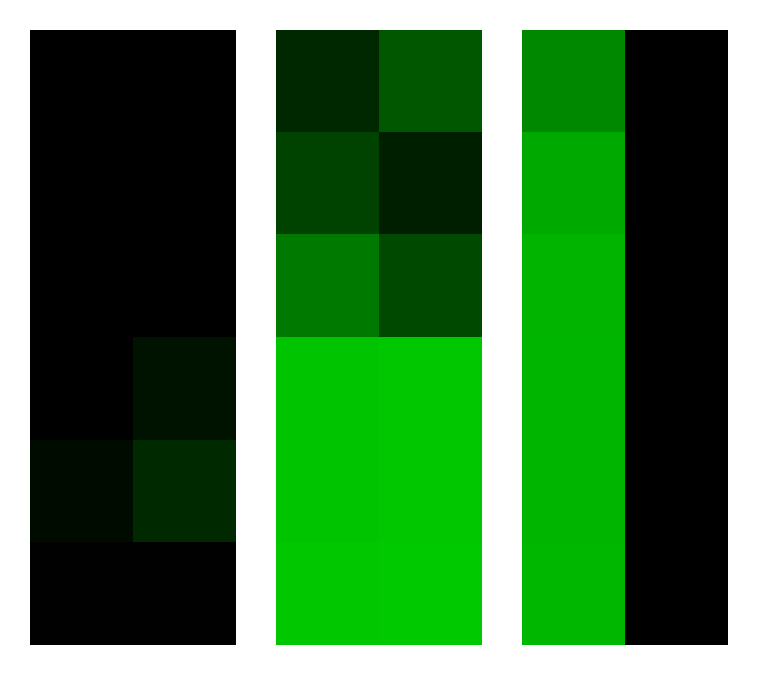
\includegraphics[width=0.3\linewidth]{chapter3/Linear/RGB_convs_2_RM_CI.png}}
    ~
    \subcaptionbox
        {
        \label{fig:linear-RM-CI-gray-2}}
        {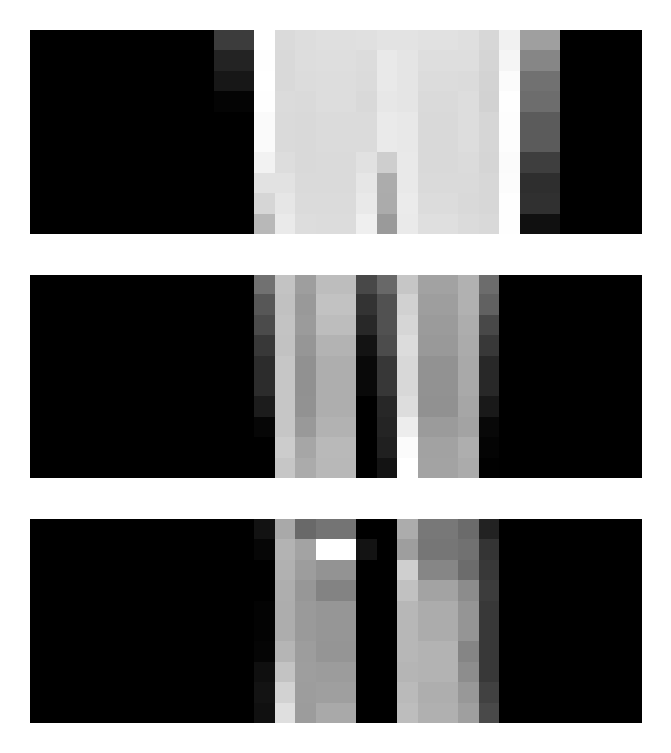
\includegraphics[width=0.3\linewidth]{chapter3/Linear/Gray_convs_2_RM_CI.png}}
    \caption{輸入影像與色彩特徵傳遞區塊和輪廓特徵傳遞區塊最後一層的RM-CI (a)輸入影像;(b)RM-CI-Color-2;(c)RM-CI-Gray-2}
    \label{fig:RM-CI}
\end{figure}

\begin{figure}[H]
    \centering
    \subcaptionbox
        {
        \label{fig:linear-rgb}}
        {
\includegraphics[width=0.33\linewidth]{chapter3/Linear/Linear_color.png}}
    ~
    \subcaptionbox
        {
        \label{fig:linear-gray}}
        {
\includegraphics[width=0.33\linewidth]{chapter3/Linear/Linear_gray.png}}
    \caption{輸入影像與色彩特徵傳遞區塊和輪廓特徵傳遞區塊最後一層的RM-CI (a) x * w 最大位置色彩CI;(b) x * w 最大位置輪廓CI}
    \label{fig:Linear-w-x}
\end{figure}

\end{document}          % 研究方法
        \documentclass[class=NCU\_thesis, crop=false]{standalone}
\usepackage{makecell}
\usepackage{diagbox}
\usepackage{longtable}
\begin{document}

\chapter{實驗設計與結果}
\section{資料集介紹}
本研究主要使用三種資料集,MNIST\cite{726791}、Colored MNIST、Colored Fashion MNIST。
MNIST和Fashion MNIST\cite{xiao2017fashionmnist}都是現在被廣泛運用在機器學習領域的資料集,
MNIST是手寫數字影像資料集、Fashion MNIST服飾影像資料集。 
Colored MNIST和Colored Fashion MNIST則是將MNIST和Fashion MNIST塗上紅、藍、綠三種不同的顏色組成。
MNIST 在本研究中用於驗證特徵傳遞模組的優化效果,
Colored MNIST和Colored Fashion主要用於驗證模型在彩色影像的分類效果。
\pagebreak
    \subsection{MNIST 資料集}
    MNIST資料集由0到9的手寫數字影像資料集組成,
    其分類具有0到9十種分類,
    影像大小為28*28並且每個影像均為灰階影像。
    該資料集共有60000筆訓練資料,10000筆測試資料

    \fig[1][fig:MNIST-Dataset-picture][H]{chapter4/MNIST.png}[MNIST資料集][MNIST資料集]
    \pagebreak
    \subsection{Colored MNIST 資料集}
    在MNIST的資料集上,塗上紅、藍、綠三種顏色,
    形成紅、藍、綠三色的0到9的彩色手寫資料集,
    其分類具有由紅藍綠和0到9排列組合成的30個分類,像是red 9、blue 6等等。
    如\cref{fig:Colored-MNIST-Dataset-picture}所示,
    該資料集共有60000筆訓練資料,10000筆測試資料。

    著色的方法如下:
    為每個灰階影像都設定一個[1,9]之間的隨機整數,
    如果隨機數小於等於3,
    則將影像的灰階值複製到彩色影像的綠色channels中並且將紅藍兩個channel設為0,
    標籤為blue加上灰階影像的數字;
    如果隨機數介於4到6之間(包含6),
    則將影像的灰階值複製到彩色影像的藍色channels中並且將紅綠兩個channel設為0,
    標籤為blue加上灰階影像的數字;
    如果隨機數大於6,
    則將影像的灰階值複製到彩色影像的紅色channels中並且將藍綠兩個channel設為0,
    標籤為red加上灰階影像的數字。

    \fig[1][fig:Colored-MNIST-Dataset-picture][H]{chapter4/Colored_MNIST.png}[Colored MNIST資料集][Colored MNIST資料集]
    \pagebreak
    \subsection{Colored Fashion MNIST 資料集}
    Fashion MNIST的資料集是由10種不同的鞋類和服裝組成的灰階影像資料集,
    其分類包含有T-Shirt/Top、Trouser、Pullover、Dress、Coat、Sandals、Shirt、Sneaker、Bag、Ankle boot等10類。
    Colored Fashion MNIST便是將Fashion MNIST資料集中的灰階影像塗上紅、藍、綠三種顏色,
    形成紅、藍、綠三色的10類服飾的彩色服飾資料集,如\cref{fig:Colored-Fashion-MNIST-Dataset-picture}。
    該資料集共有60000筆訓練資料,10000筆測試資料。

    著色的方法如下:
    為每個灰階影像都設定一個[1,9]之間的隨機整數,
    如果隨機數小於等於3,
    則將影像的灰階值複製到彩色影像的綠色channels中並且將紅藍兩個channel設為0,
    標籤為blue加上灰階影像的服飾類別;
    如果隨機數介於4到6之間(包含6),
    則將影像的灰階值複製到彩色影像的藍色channels中並且將紅綠兩個channel設為0,
    標籤為blue加上灰階影像的服飾類別;
    如果隨機數大於6,
    則將影像的灰階值複製到彩色影像的紅色channels中並且將藍綠兩個channel設為0,
    標籤為red加上灰階影像的服飾類別。

    \fig[1][fig:Colored-Fashion-MNIST-Dataset-picture][H]{chapter4/Colored Fashion MNIST.png}[Colored Fashion MNIST資料集][Colored Fashion MNIST資料集]
    \pagebreak

    \subsection{CIFAR-10 資料集}
    CIFAR-10 資料集\cite{CIFAR10} 是由各種現實影像所組成,共有10個類別,
    分別為airplane、automobile、bird、cat、deer、dog、frog、horse、ship 和 truck,
    如\cref{fig:CIFAR10},
    每個影像為彩色圖像,解析度為 28 * 28。
    該資料集共有50000筆訓練資料,10000筆測試資料。

    \fig[1][fig:CIFAR10][H]{chapter4/CIFAR10.png}[CIFAR10資料集\cite{CIFAR10}][CIFAR10資料集]
    \pagebreak
\section{實驗設計}
    \subsection{MNIST 實驗設計}
    首先在MNIST資料集的部分,
    由於MNIST資料集本身便是灰階影像,
    因此我們只採用了模型中的輪廓感知區塊與輪廓特徵傳遞區塊,
    並且去除前處理的灰階化和正規化去做訓練,
    輪廓感知區域固定為1層,
    輪廓特徵區塊我們設定為3層,
    因此此模型總共為四層架構。
    輪廓感知區塊的C$^{gray}_{0}$設定為100,
    輪廓特徵傳遞區塊的C$^{gray}_{1}$、C$^{gray}_{2}$、C$^{gray}_{3}$分別設定為225、625、1225。
    其餘相關參數的設定如\cref{tab:GrayModelparameters},其中L代表著模型的總層數,
    也就是輪廓感知區塊的層數加上輪廓特徵傳遞區塊的層數,
    以第0層代表輪廓感知區塊、第1~$\sim$ L-1層則屬於輪廓特徵傳遞區塊;
    $Filter_{i}$代表第0~$\sim$ L-1層中高斯卷積模組中的濾波器大小;
    $stride_{i}$代表第0~$\sim$ L-1層中高斯卷積模組中的步長;
    $p_{i}$代表第0~$\sim$ L-1層中響應篩選模組中希望保留的$RM$元素的百分比參數 $p\%$;
    $SF_{i}$代表第0~$\sim$ L-2層中空間濾波器的大小並且在(L-1)層不進行空間合併。

    \fig[1][fig:mnist_gray_arch][H]{Chapter4/MNIST_arch.png}[MNIST實驗模型架構圖][MNIST實驗模型架構圖]

    \begin{table}[H]
        \centering
        \caption{實驗參數設定}
        \label{tab:GrayModelparameters}
        \begin{tabular}{| c | c |}
            \hline
            參數 & 設定值 \\
            \hline
            \hline
            影像大小 & $28\times28$ \\
            \hline
            影像類別數量 & 10 \\
            \hline
            訓練批次大小 & 256 \\
            \hline
            訓練迭代次數 & 200 \\
            \hline
            優化器 & Adam \\
            \hline
            學習率 & 0.001 \\
            \hline
            損失函數 & Cross Entropy \\
            \hline
            L(層數) & 4 \\
            \hline
            i & 1 to L \\
            \hline
            $Filter\_{i}$ & $\left\{(5, 5), (1, 1), (1, 1), (1, 1)\right\}$ \\
            \hline 
            $stride\_{i}$ &$\left\{(4, 4), (1, 1), (1, 1), (1, 1)\right\}$ \\
            \hline
            $p\_{i}$ & $\left\{0.2, 0.3, 0.4, 0.5\right\}$ \\
            \hline
            $SF\_{i}$ &  \makecell{$\left\{(2, 2), (1, 3), (3, 1)\right\}$ }  \\
            \hline 
        \end{tabular}
    \end{table}


    \subsection{彩色資料集實驗設計}
    \label{chapter:ColoredModel}
    \fig[1][fig:color_model_arch][H]{model_arch.png}[彩色實驗架構圖][彩色實驗架構圖]
    我們將使用Colored MNIST 和Colored Fashion MNIST 資料集的實驗稱為彩色資料集實驗。
    在彩色資料集實驗中,
    我們設定色彩特徵傳遞區塊為兩層,
    其濾波器數目由前到後將C$^{color}_{1}$、C$^{color}_{2}$分別設定為225、625;
    輪廓感知區塊固定一層,其濾波器數目C$^{gray}_{0}$設定為70;
    輪廓特徵傳遞區塊設定為兩層,
    其濾波器數目由前到後將C$^{gray}_{1}$、C$^{gray}_{2}$分別設定為625、1225。
    其架構如\cref{fig:color_model_arch}。

    為了方便人們對於模型去進行理解和色彩與輪廓解釋性圖片的對應,
    在色彩感知區塊和輪廓感知區塊我們會使用相同濾波器大小、相同步長,
    在色彩特徵傳遞區塊和輪廓特徵傳遞區塊我們會維持相同的層數、相同的空間濾波器的大小,
    來讓色彩特徵傳遞區塊和輪廓特徵傳遞區塊的CI維持相同的大小。
    其餘相關參數設定如\cref{tab:ColoredModelparameters},
    其中的L代表著色彩和輪廓的層數,
    色彩的第0層代表著色彩感知區塊,第1~$\sim$L-1層屬於色彩特徵傳遞區塊;
    輪廓的第0層代表著輪廓感知區塊,第1~$\sim$L-1層屬於輪廓特徵傳遞區塊;
    $Filter_{i}$代表第0~$\sim$ L-1層中高斯卷積模組中的濾波器大小;
    $stride_{i}$代表第0~$\sim$ L-1層中高斯卷積模組中的步長;
    $p_{i}$代表輪廓與色彩第0~$\sim$ L-1層中響應篩選模組中希望保留的$RM$元素的百分比參數 $p\%$;
    $SF_{i}$代表第0~$\sim$ L-2層中空間濾波器的大小並且在(L-1)層不進行空間合併。

    \begin{table}[H]
        \centering
        \caption{實驗參數設定}
        \label{tab:ColoredModelparameters}
        \begin{tabular}{| c | c |}
            \hline
            參數 & 設定值 \\
            \hline
            \hline
            影像大小 & $28\times28$ \\
            \hline
            影像類別數量 & 30 \\
            \hline
            訓練批次大小 & 256 \\
            \hline
            訓練迭代次數 & 200 \\
            \hline
            優化器 & Adam \\
            \hline
            學習率 & 0.001 \\
            \hline
            損失函數 & Cross Entropy \\
            \hline
            L(層數) & 3 \\
            \hline
            i & 1 to L \\
            \hline
            $Filter\_{i}$ & \makecell{色彩 $\left\{(5, 5), (1, 1), (1, 1)\right\}$ \\ 輪廓 $\left\{(5, 5), (1, 1), (1, 1)\right\}$ }\\
            \hline 
            $stride\_{i}$ & \makecell{色彩 $\left\{(4, 4), (1, 1), (1, 1)\right\}$ \\ 輪廓 $\left\{(4, 4), (1, 1), (1, 1)\right\}$ } \\
            \hline
            $p\_{i}$ & \makecell{色彩 $\left\{0.3, 0.4, 0.5\right\}$  \\ 輪廓 $\left\{0.3, 0.4, 0.5\right\}$ } \\
            \hline
            $SF\_{i}$ &  \makecell{色彩 $\left\{(2, 2), (1, 3)\right\}$ \\ 輪廓 $\left\{(2, 2), (1, 3)\right\}$ }  \\
            \hline 
        \end{tabular}
    \end{table} 
    \pagebreak

    \subsection{CIFAR10實驗設計}
    由於現實影像的特徵複雜度較為複雜,
    在CIFAR10實驗中我們將色彩區塊和輪廓區塊的濾波器數目增多,
    我們設定色彩特徵傳遞區塊為二層,
    其濾波器數目由前到後將C$^{color}_{1}$、C$^{color}_{2}$分別設定為225、625;
    輪廓感知區塊固定一層,其濾波器數目C$^{gray}_{0}$設定為100;
    輪廓特徵傳遞區塊設定為兩層,
    其濾波器數目由前到後將C$^{gray}_{1}$、C$^{gray}_{2}$分別設定為1225、2500。
    其餘相關參數設定和彩色資料集實驗相同,如\cref{tab:ColoredModelparameters}。

\section{實驗結果}
    \subsection{實驗結果資料}
    本實驗的模型將與CIM、AlexNet\cite{NIPS2012_c399862d}、ResNet-18\cite{He_2016_CVPR}、GoogLeNet\cite{Szegedy_2015_CVPR}、DenseNet\cite{Huang_2017_CVPR}在 MNIST 資料集上進行比較。

    為了後面比較CIM和本模型的訓練時間與效果,
    我們將CIM和我們的模型設定的盡可能相近,
    CIM的參數設定如下:
    濾波器數目$C^{1}_{out}$、$C^{2}_{out}$、$C^{3}_{out}$、$C^{4}_{out}$ 設定為$100$、$225$、$625$和$1225$,
    c(整流線性單位函數的閥值)設定為 0.4, 0.1, 0.1, 0.1,
    kerenl大小設定為(5,5), (10,10), (15,15), (25,25), 
    stirde設定為(4,4), (1,1), (1,1), (1,1),
    合併SF設定為為(2,2), (1,3), (3,1)。

    但由於CIM無法處理彩色影像,因此我們在Colored MNIST與Colored Fashion MNIST 資料集上,
    將比較本模型、AlexNet、ResNet\-18、GoogLeNet、DenseNet等四種模型效果,
    以上的模型均執行 200 epochs,learning rate = 0.001。

    \begin{table}[H]
        \centering
        \caption{實驗結果}
        \label{tab:results}
        \begin{tabular}{| c | c | c | c |}
            \hline
            Dataset & Model  & \makecell{訓練準確率 \\ (60000張)} & \makecell{測試準確率 \\ (10000張)}  \\
            \hline
            \multirow{6}*{\makecell{MNIST \\ (28x28)}} 
              & Ours & 0.9621 & 0.9566 \\
            ~ & CIM~\cite{YangCNNInterpretable} & 0.9453 & 0.9368 \\
            ~ & AlexNet~\cite{NIPS2012_c399862d} & 1.0 & 0.9942   \\            
            ~ & ResNet18~\cite{He_2016_CVPR} & 1.0 & 0.9895   \\
            ~ & GoogLeNet~\cite{Szegedy_2015_CVPR} & 1.0 & 0.9943   \\
            ~ & DenseNet~\cite{Huang_2017_CVPR} & 1.0 & 0.9944   \\
            \hline
            \multirow{5}*{\makecell{Colored MNIST \\ (28x28)}} 
            & Ours & 0.9795 & 0.954 \\
            ~ & AlexNet~\cite{NIPS2012_c399862d} & 1.0 & 0.991   \\
            ~ & ResNet18~\cite{He_2016_CVPR} & 1.0  & 0.9822   \\
            ~ & GoogLeNet~\cite{Szegedy_2015_CVPR} & 1.0 & 0.9927   \\
            ~ & DenseNet~\cite{Huang_2017_CVPR} & 1.0 & 0.993   \\
            \hline
            \multirow{5}*{\makecell{Colored Fashion MNIST \\ (28x28)}} 
            & Ours & 0.8847 & 0.8223 \\
            ~ & AlexNet~\cite{NIPS2012_c399862d} & 0.9992 & 0.8973   \\
            ~ & ResNet18~\cite{He_2016_CVPR} & 1.0 & 0.8792   \\
            ~ & GoogLeNet~\cite{Szegedy_2015_CVPR} & 1.0 & 0.898   \\
            ~ & DenseNet~\cite{Huang_2017_CVPR} & 1.0 &  0.9012 \\
            \hline
            \multirow{5}*{\makecell{CIFAR10 \\ (28x28)}} 
            & Ours & 0.5918 & 0.5012 \\
            ~ & AlexNet~\cite{NIPS2012_c399862d} & 0.9992 & 0.7592   \\
            ~ & ResNet18~\cite{He_2016_CVPR} & 0.9781 & 0.7591   \\
            ~ & GoogLeNet~\cite{Szegedy_2015_CVPR} & 1.0 & 0.7696   \\
            ~ & DenseNet~\cite{Huang_2017_CVPR} & 1.0 &  0.8485 \\
            \hline
        \end{tabular}   
    \end{table}

    \pagebreak
    \subsection{可解釋性圖片}
    在本章中,我們將展示MNIST、Colored MNIST和Colored Fashion MNIST三個資料集的可解釋性圖片範例。
    由於模型在CIFAR10資料集上的準確度較低,
    表明模型未能充分學習到該資料集的特徵,
    呈現可解釋性圖片沒有實際意義,
    因此改為於\cref{chapter:failureAnalysis}分析其學習失敗的原因。

    下面表格的符號意義:
    \begin{description}
        \item[RM-CI-Color-0] 為色彩感知區塊根據RM$^{color}_{0}$每一張RM選擇最大的反應並在CI$^{color}_{0}$的對應位置中找到的CI影像;
        \item[RM-CI-Color-1] 為色彩特徵傳遞區塊的第一層根據RM$^{color}_{1}$每一張RM選擇最大的反應並在CI$^{color}_{1}$的對應位置中找到的CI影像;
        \item[RM-CI-Color-2] 為色彩特徵傳遞區塊的第二層根據RM$^{color}_{2}$每一張RM選擇最大的反應並在CI$^{color}_{2}$的對應位置中找到的CI影像;

        \item[RM-CI-Gray-0] 為輪廓感知區塊根據RM$^{gray}_{0}$每一張RM選擇最大的反應並在CI$^{gray}_{0}$的對應位置中找到的CI影像;
        \item[RM-CI-Gray-1] 為輪廓特徵傳遞區塊的第一層根據RM$^{gray}_{1}$每一張RM選擇最大的反應並在CI$^{gray}_{1}$的對應位置中找到的CI影像;
        \item[RM-CI-Gray-2] 為輪廓特徵傳遞區塊的第二層根據RM$^{gray}_{2}$每一張RM選擇最大的反應並在CI$^{gray}_{2}$的對應位置中找到的CI影像;
    \end{description}
    以下的三張表格為模型在三種資料集的30類中各類別所獲得的可解釋性圖形。
    我們從以下的結果可以觀察出,當我們獲得某一層的RM時,我們確實可以從RM對應到FM,再找到對應的CI來幫助我們理解FM所學習到的特徵,由此觀察到模型在輸入影像中特定部分學習到的特徵,解析模型的決策。
    \pagebreak
    {\small
    \begin{longtable}{|c|c|c|c|c|c|}
        \endfoot
        \caption{本研究之模型在 MNIST 上 可解釋性圖片}
        \label{tab:MNIST-pictures} \\
        \hline
        Label & Input & RM-CI-Gray-0 & RM-CI-Gray-1 & RM-CI-Gray-2 &RM-CI-Gray-3\\
        \hline
        0 & 
        \begin{minipage}[t]{0.05\columnwidth}\centering
\includegraphics[width=1\textwidth]{mnist_0506_SFMCNN_best_9edhqpk5_our/example/0/origin.png}\end{minipage} & 
        \begin{minipage}[t]{0.05\columnwidth}\centering\includegraphics[width=1\textwidth]{mnist_0506_SFMCNN_best_9edhqpk5_our/example/0/Layer0_RM_CI.png}\end{minipage} & 
        \begin{minipage}[t]{0.05\columnwidth}\centering
\includegraphics[width=1\textwidth]{mnist_0506_SFMCNN_best_9edhqpk5_our/example/0/Layer1_RM_CI.png}\end{minipage} & 
        \begin{minipage}[t]{0.05\columnwidth}\centering
\includegraphics[width=1\textwidth]{mnist_0506_SFMCNN_best_9edhqpk5_our/example/0/Layer2_RM_CI.png}\end{minipage} & 
        \begin{minipage}[t]{0.05\columnwidth}\centering
\includegraphics[width=1\textwidth]{mnist_0506_SFMCNN_best_9edhqpk5_our/example/0/Layer3_RM_CI.png}\end{minipage} \\
        \hline
        1 & 
        \begin{minipage}[t]{0.05\columnwidth}\centering
\includegraphics[width=1\textwidth]{mnist_0506_SFMCNN_best_9edhqpk5_our/example/1/origin.png}\end{minipage} & 
        \begin{minipage}[t]{0.05\columnwidth}\centering\includegraphics[width=1\textwidth]{mnist_0506_SFMCNN_best_9edhqpk5_our/example/1/Layer0_RM_CI.png}\end{minipage} & 
        \begin{minipage}[t]{0.05\columnwidth}\centering
\includegraphics[width=1\textwidth]{mnist_0506_SFMCNN_best_9edhqpk5_our/example/1/Layer1_RM_CI.png}\end{minipage} & 
        \begin{minipage}[t]{0.05\columnwidth}\centering
\includegraphics[width=1\textwidth]{mnist_0506_SFMCNN_best_9edhqpk5_our/example/1/Layer2_RM_CI.png}\end{minipage} & 
        \begin{minipage}[t]{0.05\columnwidth}\centering
\includegraphics[width=1\textwidth]{mnist_0506_SFMCNN_best_9edhqpk5_our/example/1/Layer3_RM_CI.png}\end{minipage} \\
        \hline
        2 & 
        \begin{minipage}[t]{0.05\columnwidth}\centering
\includegraphics[width=1\textwidth]{mnist_0506_SFMCNN_best_9edhqpk5_our/example/2/origin.png}\end{minipage} & 
        \begin{minipage}[t]{0.05\columnwidth}\centering\includegraphics[width=1\textwidth]{mnist_0506_SFMCNN_best_9edhqpk5_our/example/2/Layer0_RM_CI.png}\end{minipage} & 
        \begin{minipage}[t]{0.05\columnwidth}\centering\includegraphics[width=1\textwidth]{mnist_0506_SFMCNN_best_9edhqpk5_our/example/2/Layer1_RM_CI.png}\end{minipage} & 
        \begin{minipage}[t]{0.05\columnwidth}\centering\includegraphics[width=1\textwidth]{mnist_0506_SFMCNN_best_9edhqpk5_our/example/2/Layer2_RM_CI.png}\end{minipage} & 
        \begin{minipage}[t]{0.05\columnwidth}\centering\includegraphics[width=1\textwidth]{mnist_0506_SFMCNN_best_9edhqpk5_our/example/2/Layer3_RM_CI.png}\end{minipage} \\
        \hline
        3 & 
        \begin{minipage}[t]{0.05\columnwidth}\centering\includegraphics[width=1\textwidth]{mnist_0506_SFMCNN_best_9edhqpk5_our/example/3/origin.png}\end{minipage} & 
        \begin{minipage}[t]{0.05\columnwidth}\centering\includegraphics[width=1\textwidth]{mnist_0506_SFMCNN_best_9edhqpk5_our/example/3/Layer0_RM_CI.png}\end{minipage} & 
        \begin{minipage}[t]{0.05\columnwidth}\centering\includegraphics[width=1\textwidth]{mnist_0506_SFMCNN_best_9edhqpk5_our/example/3/Layer1_RM_CI.png}\end{minipage} & 
        \begin{minipage}[t]{0.05\columnwidth}\centering\includegraphics[width=1\textwidth]{mnist_0506_SFMCNN_best_9edhqpk5_our/example/3/Layer2_RM_CI.png}\end{minipage} & 
        \begin{minipage}[t]{0.05\columnwidth}\centering\includegraphics[width=1\textwidth]{mnist_0506_SFMCNN_best_9edhqpk5_our/example/3/Layer3_RM_CI.png}\end{minipage} \\
        \hline
        4 & 
        \begin{minipage}[t]{0.05\columnwidth}\centering\includegraphics[width=1\textwidth]{mnist_0506_SFMCNN_best_9edhqpk5_our/example/4/origin.png}\end{minipage} & 
        \begin{minipage}[t]{0.05\columnwidth}\centering\includegraphics[width=1\textwidth]{mnist_0506_SFMCNN_best_9edhqpk5_our/example/4/Layer0_RM_CI.png}\end{minipage} & 
        \begin{minipage}[t]{0.05\columnwidth}\centering\includegraphics[width=1\textwidth]{mnist_0506_SFMCNN_best_9edhqpk5_our/example/4/Layer1_RM_CI.png}\end{minipage} & 
        \begin{minipage}[t]{0.05\columnwidth}\centering\includegraphics[width=1\textwidth]{mnist_0506_SFMCNN_best_9edhqpk5_our/example/4/Layer2_RM_CI.png}\end{minipage} & 
        \begin{minipage}[t]{0.05\columnwidth}\centering\includegraphics[width=1\textwidth]{mnist_0506_SFMCNN_best_9edhqpk5_our/example/4/Layer3_RM_CI.png}\end{minipage} \\
        \hline
        5 & 
        \begin{minipage}[t]{0.05\columnwidth}\centering\includegraphics[width=1\textwidth]{mnist_0506_SFMCNN_best_9edhqpk5_our/example/5/origin.png}\end{minipage} & 
        \begin{minipage}[t]{0.05\columnwidth}\centering\includegraphics[width=1\textwidth]{mnist_0506_SFMCNN_best_9edhqpk5_our/example/5/Layer0_RM_CI.png}\end{minipage} & 
        \begin{minipage}[t]{0.05\columnwidth}\centering\includegraphics[width=1\textwidth]{mnist_0506_SFMCNN_best_9edhqpk5_our/example/5/Layer1_RM_CI.png}\end{minipage} & 
        \begin{minipage}[t]{0.05\columnwidth}\centering\includegraphics[width=1\textwidth]{mnist_0506_SFMCNN_best_9edhqpk5_our/example/5/Layer2_RM_CI.png}\end{minipage} & 
        \begin{minipage}[t]{0.05\columnwidth}\centering\includegraphics[width=1\textwidth]{mnist_0506_SFMCNN_best_9edhqpk5_our/example/5/Layer3_RM_CI.png}\end{minipage} \\
        \hline
        6 & 
        \begin{minipage}[t]{0.05\columnwidth}\centering\includegraphics[width=1\textwidth]{mnist_0506_SFMCNN_best_9edhqpk5_our/example/6/origin.png}\end{minipage} & 
        \begin{minipage}[t]{0.05\columnwidth}\centering\includegraphics[width=1\textwidth]{mnist_0506_SFMCNN_best_9edhqpk5_our/example/6/Layer0_RM_CI.png}\end{minipage} & 
        \begin{minipage}[t]{0.05\columnwidth}\centering\includegraphics[width=1\textwidth]{mnist_0506_SFMCNN_best_9edhqpk5_our/example/6/Layer1_RM_CI.png}\end{minipage} & 
        \begin{minipage}[t]{0.05\columnwidth}\centering\includegraphics[width=1\textwidth]{mnist_0506_SFMCNN_best_9edhqpk5_our/example/6/Layer2_RM_CI.png}\end{minipage} & 
        \begin{minipage}[t]{0.05\columnwidth}\centering\includegraphics[width=1\textwidth]{mnist_0506_SFMCNN_best_9edhqpk5_our/example/6/Layer3_RM_CI.png}\end{minipage} \\
        \hline
        7 & 
        \begin{minipage}[t]{0.05\columnwidth}\centering\includegraphics[width=1\textwidth]{mnist_0506_SFMCNN_best_9edhqpk5_our/example/7/origin.png}\end{minipage} & 
        \begin{minipage}[t]{0.05\columnwidth}\centering\includegraphics[width=1\textwidth]{mnist_0506_SFMCNN_best_9edhqpk5_our/example/7/Layer0_RM_CI.png}\end{minipage} & 
        \begin{minipage}[t]{0.05\columnwidth}\centering\includegraphics[width=1\textwidth]{mnist_0506_SFMCNN_best_9edhqpk5_our/example/7/Layer1_RM_CI.png}\end{minipage} & 
        \begin{minipage}[t]{0.05\columnwidth}\centering\includegraphics[width=1\textwidth]{mnist_0506_SFMCNN_best_9edhqpk5_our/example/7/Layer2_RM_CI.png}\end{minipage} & 
        \begin{minipage}[t]{0.05\columnwidth}\centering\includegraphics[width=1\textwidth]{mnist_0506_SFMCNN_best_9edhqpk5_our/example/7/Layer3_RM_CI.png}\end{minipage} \\
        \hline
        8 & 
        \begin{minipage}[t]{0.05\columnwidth}\centering\includegraphics[width=1\textwidth]{mnist_0506_SFMCNN_best_9edhqpk5_our/example/8/origin.png}\end{minipage} & 
        \begin{minipage}[t]{0.05\columnwidth}\centering\includegraphics[width=1\textwidth]{mnist_0506_SFMCNN_best_9edhqpk5_our/example/8/Layer0_RM_CI.png}\end{minipage} & 
        \begin{minipage}[t]{0.05\columnwidth}\centering\includegraphics[width=1\textwidth]{mnist_0506_SFMCNN_best_9edhqpk5_our/example/8/Layer1_RM_CI.png}\end{minipage} & 
        \begin{minipage}[t]{0.05\columnwidth}\centering\includegraphics[width=1\textwidth]{mnist_0506_SFMCNN_best_9edhqpk5_our/example/8/Layer2_RM_CI.png}\end{minipage} & 
        \begin{minipage}[t]{0.05\columnwidth}\centering\includegraphics[width=1\textwidth]{mnist_0506_SFMCNN_best_9edhqpk5_our/example/8/Layer3_RM_CI.png}\end{minipage} \\
        \hline
        9 & 
        \begin{minipage}[t]{0.05\columnwidth}\centering\includegraphics[width=1\textwidth]{mnist_0506_SFMCNN_best_9edhqpk5_our/example/9/origin.png}\end{minipage} & 
        \begin{minipage}[t]{0.05\columnwidth}\centering\includegraphics[width=1\textwidth]{mnist_0506_SFMCNN_best_9edhqpk5_our/example/9/Layer0_RM_CI.png}\end{minipage} & 
        \begin{minipage}[t]{0.05\columnwidth}\centering\includegraphics[width=1\textwidth]{mnist_0506_SFMCNN_best_9edhqpk5_our/example/9/Layer1_RM_CI.png}\end{minipage} & 
        \begin{minipage}[t]{0.05\columnwidth}\centering\includegraphics[width=1\textwidth]{mnist_0506_SFMCNN_best_9edhqpk5_our/example/9/Layer2_RM_CI.png}\end{minipage} & 
        \begin{minipage}[t]{0.05\columnwidth}\centering\includegraphics[width=1\textwidth]{mnist_0506_SFMCNN_best_9edhqpk5_our/example/9/Layer3_RM_CI.png}\end{minipage} \\
        \hline
    \end{longtable}

    \pagebreak
    
    \begin{longtable}{|c|c|c|c|c|}
        \endfoot
        \caption{本研究之模型在 Colored MNIST 上 可解釋性圖片}
        \label{tab:coloredMNIST-pictures}\\
            \hline
            \multirow{2}*{Label} & \multirow{2}*{Input} & RM-CI-Color-0 & RM-CI-Color-1 & RM-CI-Color-2 \\
            \cline{3-5}
            & & RM-CI-Gray-0 & RM-CI-Gray-1 & RM-CI-Gray-2\\
            \hline
            \multirow{2}*{red\_0} & 
            \multirow{2}*{\begin{minipage}[t]{0.05\columnwidth}\centering\includegraphics[width=1\textwidth]{Colored_MNIST_0610_RGB_SFMCNN_best_t1np8eon_LAB/example/red_0/origin.png}\end{minipage}} & 
            \begin{minipage}[t]{0.05\columnwidth}\centering\includegraphics[width=1\textwidth]{Colored_MNIST_0610_RGB_SFMCNN_best_t1np8eon_LAB/example/red_0/RGB_convs_0_RM_CI.png}\end{minipage} &
            \begin{minipage}[t]{0.05\columnwidth}\centering\includegraphics[width=1\textwidth]{Colored_MNIST_0610_RGB_SFMCNN_best_t1np8eon_LAB/example/red_0/RGB_convs_1_RM_CI.png}\end{minipage} &
            \begin{minipage}[t]{0.05\columnwidth}\centering\includegraphics[width=1\textwidth]{Colored_MNIST_0610_RGB_SFMCNN_best_t1np8eon_LAB/example/red_0/RGB_convs_2_RM_CI.png}\end{minipage} \\
            \cline{3-5}
            & & 
            \begin{minipage}[t]{0.05\columnwidth}\centering\includegraphics[width=1\textwidth]{Colored_MNIST_0610_RGB_SFMCNN_best_t1np8eon_LAB/example/red_0/Gray_convs_0_RM_CI.png}\end{minipage} &
            \begin{minipage}[t]{0.05\columnwidth}\centering\includegraphics[width=1\textwidth]{Colored_MNIST_0610_RGB_SFMCNN_best_t1np8eon_LAB/example/red_0/Gray_convs_1_RM_CI.png}\end{minipage} &
            \begin{minipage}[t]{0.05\columnwidth}\centering\includegraphics[width=1\textwidth]{Colored_MNIST_0610_RGB_SFMCNN_best_t1np8eon_LAB/example/red_0/Gray_convs_2_RM_CI.png}\end{minipage} \\
            \hline

            \multirow{2}*{red\_1} & 
            \multirow{2}*{\begin{minipage}[t]{0.05\columnwidth}\centering\includegraphics[width=1\textwidth]{Colored_MNIST_0610_RGB_SFMCNN_best_t1np8eon_LAB/example/red_1/origin.png}\end{minipage}} & 
            \begin{minipage}[t]{0.05\columnwidth}\centering\includegraphics[width=1\textwidth]{Colored_MNIST_0610_RGB_SFMCNN_best_t1np8eon_LAB/example/red_1/RGB_convs_0_RM_CI.png}\end{minipage} &
            \begin{minipage}[t]{0.05\columnwidth}\centering\includegraphics[width=1\textwidth]{Colored_MNIST_0610_RGB_SFMCNN_best_t1np8eon_LAB/example/red_1/RGB_convs_1_RM_CI.png}\end{minipage} &
            \begin{minipage}[t]{0.05\columnwidth}\centering\includegraphics[width=1\textwidth]{Colored_MNIST_0610_RGB_SFMCNN_best_t1np8eon_LAB/example/red_1/RGB_convs_2_RM_CI.png}\end{minipage} \\
            \cline{3-5}
            & & 
            \begin{minipage}[t]{0.05\columnwidth}\centering\includegraphics[width=1\textwidth]{Colored_MNIST_0610_RGB_SFMCNN_best_t1np8eon_LAB/example/red_1/Gray_convs_0_RM_CI.png}\end{minipage} &
            \begin{minipage}[t]{0.05\columnwidth}\centering\includegraphics[width=1\textwidth]{Colored_MNIST_0610_RGB_SFMCNN_best_t1np8eon_LAB/example/red_1/Gray_convs_1_RM_CI.png}\end{minipage} &
            \begin{minipage}[t]{0.05\columnwidth}\centering\includegraphics[width=1\textwidth]{Colored_MNIST_0610_RGB_SFMCNN_best_t1np8eon_LAB/example/red_1/Gray_convs_2_RM_CI.png}\end{minipage} \\
            \hline

            \multirow{2}*{red\_2} & 
            \multirow{2}*{\begin{minipage}[t]{0.05\columnwidth}\centering\includegraphics[width=1\textwidth]{Colored_MNIST_0610_RGB_SFMCNN_best_t1np8eon_LAB/example/red_2/origin.png}\end{minipage}} & 
            \begin{minipage}[t]{0.05\columnwidth}\centering\includegraphics[width=1\textwidth]{Colored_MNIST_0610_RGB_SFMCNN_best_t1np8eon_LAB/example/red_2/RGB_convs_0_RM_CI.png}\end{minipage} &
            \begin{minipage}[t]{0.05\columnwidth}\centering\includegraphics[width=1\textwidth]{Colored_MNIST_0610_RGB_SFMCNN_best_t1np8eon_LAB/example/red_2/RGB_convs_1_RM_CI.png}\end{minipage} &
            \begin{minipage}[t]{0.05\columnwidth}\centering\includegraphics[width=1\textwidth]{Colored_MNIST_0610_RGB_SFMCNN_best_t1np8eon_LAB/example/red_2/RGB_convs_2_RM_CI.png}\end{minipage} \\
            \cline{3-5}
            & & 
            \begin{minipage}[t]{0.05\columnwidth}\centering\includegraphics[width=1\textwidth]{Colored_MNIST_0610_RGB_SFMCNN_best_t1np8eon_LAB/example/red_2/Gray_convs_0_RM_CI.png}\end{minipage} &
            \begin{minipage}[t]{0.05\columnwidth}\centering\includegraphics[width=1\textwidth]{Colored_MNIST_0610_RGB_SFMCNN_best_t1np8eon_LAB/example/red_2/Gray_convs_1_RM_CI.png}\end{minipage} &
            \begin{minipage}[t]{0.05\columnwidth}\centering\includegraphics[width=1\textwidth]{Colored_MNIST_0610_RGB_SFMCNN_best_t1np8eon_LAB/example/red_2/Gray_convs_2_RM_CI.png}\end{minipage} \\
            \hline

            \multirow{2}*{red\_3} & 
            \multirow{2}*{\begin{minipage}[t]{0.05\columnwidth}\centering\includegraphics[width=1\textwidth]{Colored_MNIST_0610_RGB_SFMCNN_best_t1np8eon_LAB/example/red_3/origin.png}\end{minipage}} & 
            \begin{minipage}[t]{0.05\columnwidth}\centering\includegraphics[width=1\textwidth]{Colored_MNIST_0610_RGB_SFMCNN_best_t1np8eon_LAB/example/red_3/RGB_convs_0_RM_CI.png}\end{minipage} &
            \begin{minipage}[t]{0.05\columnwidth}\centering\includegraphics[width=1\textwidth]{Colored_MNIST_0610_RGB_SFMCNN_best_t1np8eon_LAB/example/red_3/RGB_convs_1_RM_CI.png}\end{minipage} &
            \begin{minipage}[t]{0.05\columnwidth}\centering\includegraphics[width=1\textwidth]{Colored_MNIST_0610_RGB_SFMCNN_best_t1np8eon_LAB/example/red_3/RGB_convs_2_RM_CI.png}\end{minipage} \\
            \cline{3-5}
            & & 
            \begin{minipage}[t]{0.05\columnwidth}\centering\includegraphics[width=1\textwidth]{Colored_MNIST_0610_RGB_SFMCNN_best_t1np8eon_LAB/example/red_3/Gray_convs_0_RM_CI.png}\end{minipage} &
            \begin{minipage}[t]{0.05\columnwidth}\centering\includegraphics[width=1\textwidth]{Colored_MNIST_0610_RGB_SFMCNN_best_t1np8eon_LAB/example/red_3/Gray_convs_1_RM_CI.png}\end{minipage} &
            \begin{minipage}[t]{0.05\columnwidth}\centering\includegraphics[width=1\textwidth]{Colored_MNIST_0610_RGB_SFMCNN_best_t1np8eon_LAB/example/red_3/Gray_convs_2_RM_CI.png}\end{minipage} \\
            \hline

            \multirow{2}*{red\_4} & 
            \multirow{2}*{\begin{minipage}[t]{0.05\columnwidth}\centering\includegraphics[width=1\textwidth]{Colored_MNIST_0610_RGB_SFMCNN_best_t1np8eon_LAB/example/red_4/origin.png}\end{minipage}} & 
            \begin{minipage}[t]{0.05\columnwidth}\centering\includegraphics[width=1\textwidth]{Colored_MNIST_0610_RGB_SFMCNN_best_t1np8eon_LAB/example/red_4/RGB_convs_0_RM_CI.png}\end{minipage} &
            \begin{minipage}[t]{0.05\columnwidth}\centering\includegraphics[width=1\textwidth]{Colored_MNIST_0610_RGB_SFMCNN_best_t1np8eon_LAB/example/red_4/RGB_convs_1_RM_CI.png}\end{minipage} &
            \begin{minipage}[t]{0.05\columnwidth}\centering\includegraphics[width=1\textwidth]{Colored_MNIST_0610_RGB_SFMCNN_best_t1np8eon_LAB/example/red_4/RGB_convs_2_RM_CI.png}\end{minipage} \\
            \cline{3-5}
            & & 
            \begin{minipage}[t]{0.05\columnwidth}\centering\includegraphics[width=1\textwidth]{Colored_MNIST_0610_RGB_SFMCNN_best_t1np8eon_LAB/example/red_4/Gray_convs_0_RM_CI.png}\end{minipage} &
            \begin{minipage}[t]{0.05\columnwidth}\centering\includegraphics[width=1\textwidth]{Colored_MNIST_0610_RGB_SFMCNN_best_t1np8eon_LAB/example/red_4/Gray_convs_1_RM_CI.png}\end{minipage} &
            \begin{minipage}[t]{0.05\columnwidth}\centering\includegraphics[width=1\textwidth]{Colored_MNIST_0610_RGB_SFMCNN_best_t1np8eon_LAB/example/red_4/Gray_convs_2_RM_CI.png}\end{minipage} \\
            \hline

            \multirow{2}*{red\_5} & 
            \multirow{2}*{\begin{minipage}[t]{0.05\columnwidth}\centering\includegraphics[width=1\textwidth]{Colored_MNIST_0610_RGB_SFMCNN_best_t1np8eon_LAB/example/red_5/origin.png}\end{minipage}} & 
            \begin{minipage}[t]{0.05\columnwidth}\centering\includegraphics[width=1\textwidth]{Colored_MNIST_0610_RGB_SFMCNN_best_t1np8eon_LAB/example/red_5/RGB_convs_0_RM_CI.png}\end{minipage} &
            \begin{minipage}[t]{0.05\columnwidth}\centering\includegraphics[width=1\textwidth]{Colored_MNIST_0610_RGB_SFMCNN_best_t1np8eon_LAB/example/red_5/RGB_convs_1_RM_CI.png}\end{minipage} &
            \begin{minipage}[t]{0.05\columnwidth}\centering\includegraphics[width=1\textwidth]{Colored_MNIST_0610_RGB_SFMCNN_best_t1np8eon_LAB/example/red_5/RGB_convs_2_RM_CI.png}\end{minipage} \\
            \cline{3-5}
            & & 
            \begin{minipage}[t]{0.05\columnwidth}\centering\includegraphics[width=1\textwidth]{Colored_MNIST_0610_RGB_SFMCNN_best_t1np8eon_LAB/example/red_5/Gray_convs_0_RM_CI.png}\end{minipage} &
            \begin{minipage}[t]{0.05\columnwidth}\centering\includegraphics[width=1\textwidth]{Colored_MNIST_0610_RGB_SFMCNN_best_t1np8eon_LAB/example/red_5/Gray_convs_1_RM_CI.png}\end{minipage} &
            \begin{minipage}[t]{0.05\columnwidth}\centering\includegraphics[width=1\textwidth]{Colored_MNIST_0610_RGB_SFMCNN_best_t1np8eon_LAB/example/red_5/Gray_convs_2_RM_CI.png}\end{minipage} \\
            \hline

            \multirow{2}*{red\_6} & 
            \multirow{2}*{\begin{minipage}[t]{0.05\columnwidth}\centering\includegraphics[width=1\textwidth]{Colored_MNIST_0610_RGB_SFMCNN_best_t1np8eon_LAB/example/red_6/origin.png}\end{minipage}} & 
            \begin{minipage}[t]{0.05\columnwidth}\centering\includegraphics[width=1\textwidth]{Colored_MNIST_0610_RGB_SFMCNN_best_t1np8eon_LAB/example/red_6/RGB_convs_0_RM_CI.png}\end{minipage} &
            \begin{minipage}[t]{0.05\columnwidth}\centering\includegraphics[width=1\textwidth]{Colored_MNIST_0610_RGB_SFMCNN_best_t1np8eon_LAB/example/red_6/RGB_convs_1_RM_CI.png}\end{minipage} &
            \begin{minipage}[t]{0.05\columnwidth}\centering\includegraphics[width=1\textwidth]{Colored_MNIST_0610_RGB_SFMCNN_best_t1np8eon_LAB/example/red_6/RGB_convs_2_RM_CI.png}\end{minipage} \\
            \cline{3-5}
            & & 
            \begin{minipage}[t]{0.05\columnwidth}\centering\includegraphics[width=1\textwidth]{Colored_MNIST_0610_RGB_SFMCNN_best_t1np8eon_LAB/example/red_6/Gray_convs_0_RM_CI.png}\end{minipage} &
            \begin{minipage}[t]{0.05\columnwidth}\centering\includegraphics[width=1\textwidth]{Colored_MNIST_0610_RGB_SFMCNN_best_t1np8eon_LAB/example/red_6/Gray_convs_1_RM_CI.png}\end{minipage} &
            \begin{minipage}[t]{0.05\columnwidth}\centering\includegraphics[width=1\textwidth]{Colored_MNIST_0610_RGB_SFMCNN_best_t1np8eon_LAB/example/red_6/Gray_convs_2_RM_CI.png}\end{minipage} \\
            \hline

            \multirow{2}*{red\_7} & 
            \multirow{2}*{\begin{minipage}[t]{0.05\columnwidth}\centering\includegraphics[width=1\textwidth]{Colored_MNIST_0610_RGB_SFMCNN_best_t1np8eon_LAB/example/red_7/origin.png}\end{minipage}} & 
            \begin{minipage}[t]{0.05\columnwidth}\centering\includegraphics[width=1\textwidth]{Colored_MNIST_0610_RGB_SFMCNN_best_t1np8eon_LAB/example/red_7/RGB_convs_0_RM_CI.png}\end{minipage} &
            \begin{minipage}[t]{0.05\columnwidth}\centering\includegraphics[width=1\textwidth]{Colored_MNIST_0610_RGB_SFMCNN_best_t1np8eon_LAB/example/red_7/RGB_convs_1_RM_CI.png}\end{minipage} &
            \begin{minipage}[t]{0.05\columnwidth}\centering\includegraphics[width=1\textwidth]{Colored_MNIST_0610_RGB_SFMCNN_best_t1np8eon_LAB/example/red_7/RGB_convs_2_RM_CI.png}\end{minipage} \\
            \cline{3-5}
            & & 
            \begin{minipage}[t]{0.05\columnwidth}\centering\includegraphics[width=1\textwidth]{Colored_MNIST_0610_RGB_SFMCNN_best_t1np8eon_LAB/example/red_7/Gray_convs_0_RM_CI.png}\end{minipage} &
            \begin{minipage}[t]{0.05\columnwidth}\centering\includegraphics[width=1\textwidth]{Colored_MNIST_0610_RGB_SFMCNN_best_t1np8eon_LAB/example/red_7/Gray_convs_1_RM_CI.png}\end{minipage} &
            \begin{minipage}[t]{0.05\columnwidth}\centering\includegraphics[width=1\textwidth]{Colored_MNIST_0610_RGB_SFMCNN_best_t1np8eon_LAB/example/red_7/Gray_convs_2_RM_CI.png}\end{minipage} \\
            \hline

            \multirow{2}*{red\_8} & 
            \multirow{2}*{\begin{minipage}[t]{0.05\columnwidth}\centering\includegraphics[width=1\textwidth]{Colored_MNIST_0610_RGB_SFMCNN_best_t1np8eon_LAB/example/red_8/origin.png}\end{minipage}} & 
            \begin{minipage}[t]{0.05\columnwidth}\centering\includegraphics[width=1\textwidth]{Colored_MNIST_0610_RGB_SFMCNN_best_t1np8eon_LAB/example/red_8/RGB_convs_0_RM_CI.png}\end{minipage} &
            \begin{minipage}[t]{0.05\columnwidth}\centering\includegraphics[width=1\textwidth]{Colored_MNIST_0610_RGB_SFMCNN_best_t1np8eon_LAB/example/red_8/RGB_convs_1_RM_CI.png}\end{minipage} &
            \begin{minipage}[t]{0.05\columnwidth}\centering\includegraphics[width=1\textwidth]{Colored_MNIST_0610_RGB_SFMCNN_best_t1np8eon_LAB/example/red_8/RGB_convs_2_RM_CI.png}\end{minipage} \\
            \cline{3-5}
            & & 
            \begin{minipage}[t]{0.05\columnwidth}\centering\includegraphics[width=1\textwidth]{Colored_MNIST_0610_RGB_SFMCNN_best_t1np8eon_LAB/example/red_8/Gray_convs_0_RM_CI.png}\end{minipage} &
            \begin{minipage}[t]{0.05\columnwidth}\centering\includegraphics[width=1\textwidth]{Colored_MNIST_0610_RGB_SFMCNN_best_t1np8eon_LAB/example/red_8/Gray_convs_1_RM_CI.png}\end{minipage} &
            \begin{minipage}[t]{0.05\columnwidth}\centering\includegraphics[width=1\textwidth]{Colored_MNIST_0610_RGB_SFMCNN_best_t1np8eon_LAB/example/red_8/Gray_convs_2_RM_CI.png}\end{minipage} \\
            \hline

            \multirow{2}*{red\_9} & 
            \multirow{2}*{\begin{minipage}[t]{0.05\columnwidth}\centering\includegraphics[width=1\textwidth]{Colored_MNIST_0610_RGB_SFMCNN_best_t1np8eon_LAB/example/red_9/origin.png}\end{minipage}} & 
            \begin{minipage}[t]{0.05\columnwidth}\centering\includegraphics[width=1\textwidth]{Colored_MNIST_0610_RGB_SFMCNN_best_t1np8eon_LAB/example/red_9/RGB_convs_0_RM_CI.png}\end{minipage} &
            \begin{minipage}[t]{0.05\columnwidth}\centering\includegraphics[width=1\textwidth]{Colored_MNIST_0610_RGB_SFMCNN_best_t1np8eon_LAB/example/red_9/RGB_convs_1_RM_CI.png}\end{minipage} &
            \begin{minipage}[t]{0.05\columnwidth}\centering\includegraphics[width=1\textwidth]{Colored_MNIST_0610_RGB_SFMCNN_best_t1np8eon_LAB/example/red_9/RGB_convs_2_RM_CI.png}\end{minipage} \\
            \cline{3-5}
            & & 
            \begin{minipage}[t]{0.05\columnwidth}\centering\includegraphics[width=1\textwidth]{Colored_MNIST_0610_RGB_SFMCNN_best_t1np8eon_LAB/example/red_9/Gray_convs_0_RM_CI.png}\end{minipage} &
            \begin{minipage}[t]{0.05\columnwidth}\centering\includegraphics[width=1\textwidth]{Colored_MNIST_0610_RGB_SFMCNN_best_t1np8eon_LAB/example/red_9/Gray_convs_1_RM_CI.png}\end{minipage} &
            \begin{minipage}[t]{0.05\columnwidth}\centering\includegraphics[width=1\textwidth]{Colored_MNIST_0610_RGB_SFMCNN_best_t1np8eon_LAB/example/red_9/Gray_convs_2_RM_CI.png}\end{minipage} \\
            \hline


            \multirow{2}*{green\_0} & 
            \multirow{2}*{\begin{minipage}[t]{0.05\columnwidth}\centering\includegraphics[width=1\textwidth]{Colored_MNIST_0610_RGB_SFMCNN_best_t1np8eon_LAB/example/green_0/origin.png}\end{minipage}} & 
            \begin{minipage}[t]{0.05\columnwidth}\centering\includegraphics[width=1\textwidth]{Colored_MNIST_0610_RGB_SFMCNN_best_t1np8eon_LAB/example/green_0/RGB_convs_0_RM_CI.png}\end{minipage} &
            \begin{minipage}[t]{0.05\columnwidth}\centering\includegraphics[width=1\textwidth]{Colored_MNIST_0610_RGB_SFMCNN_best_t1np8eon_LAB/example/green_0/RGB_convs_1_RM_CI.png}\end{minipage} &
            \begin{minipage}[t]{0.05\columnwidth}\centering\includegraphics[width=1\textwidth]{Colored_MNIST_0610_RGB_SFMCNN_best_t1np8eon_LAB/example/green_0/RGB_convs_2_RM_CI.png}\end{minipage} \\
            \cline{3-5}
            & & 
            \begin{minipage}[t]{0.05\columnwidth}\centering\includegraphics[width=1\textwidth]{Colored_MNIST_0610_RGB_SFMCNN_best_t1np8eon_LAB/example/green_0/Gray_convs_0_RM_CI.png}\end{minipage} &
            \begin{minipage}[t]{0.05\columnwidth}\centering\includegraphics[width=1\textwidth]{Colored_MNIST_0610_RGB_SFMCNN_best_t1np8eon_LAB/example/green_0/Gray_convs_1_RM_CI.png}\end{minipage} &
            \begin{minipage}[t]{0.05\columnwidth}\centering\includegraphics[width=1\textwidth]{Colored_MNIST_0610_RGB_SFMCNN_best_t1np8eon_LAB/example/green_0/Gray_convs_2_RM_CI.png}\end{minipage} \\
            \hline

            \multirow{2}*{green\_1} & 
            \multirow{2}*{\begin{minipage}[t]{0.05\columnwidth}\centering\includegraphics[width=1\textwidth]{Colored_MNIST_0610_RGB_SFMCNN_best_t1np8eon_LAB/example/green_1/origin.png}\end{minipage}} & 
            \begin{minipage}[t]{0.05\columnwidth}\centering\includegraphics[width=1\textwidth]{Colored_MNIST_0610_RGB_SFMCNN_best_t1np8eon_LAB/example/green_1/RGB_convs_0_RM_CI.png}\end{minipage} &
            \begin{minipage}[t]{0.05\columnwidth}\centering\includegraphics[width=1\textwidth]{Colored_MNIST_0610_RGB_SFMCNN_best_t1np8eon_LAB/example/green_1/RGB_convs_1_RM_CI.png}\end{minipage} &
            \begin{minipage}[t]{0.05\columnwidth}\centering\includegraphics[width=1\textwidth]{Colored_MNIST_0610_RGB_SFMCNN_best_t1np8eon_LAB/example/green_1/RGB_convs_2_RM_CI.png}\end{minipage} \\
            \cline{3-5}
            & & 
            \begin{minipage}[t]{0.05\columnwidth}\centering\includegraphics[width=1\textwidth]{Colored_MNIST_0610_RGB_SFMCNN_best_t1np8eon_LAB/example/green_1/Gray_convs_0_RM_CI.png}\end{minipage} &
            \begin{minipage}[t]{0.05\columnwidth}\centering\includegraphics[width=1\textwidth]{Colored_MNIST_0610_RGB_SFMCNN_best_t1np8eon_LAB/example/green_1/Gray_convs_1_RM_CI.png}\end{minipage} &
            \begin{minipage}[t]{0.05\columnwidth}\centering\includegraphics[width=1\textwidth]{Colored_MNIST_0610_RGB_SFMCNN_best_t1np8eon_LAB/example/green_1/Gray_convs_2_RM_CI.png}\end{minipage} \\
            \hline

            \multirow{2}*{green\_2} & 
            \multirow{2}*{\begin{minipage}[t]{0.05\columnwidth}\centering\includegraphics[width=1\textwidth]{Colored_MNIST_0610_RGB_SFMCNN_best_t1np8eon_LAB/example/green_2/origin.png}\end{minipage}} & 
            \begin{minipage}[t]{0.05\columnwidth}\centering\includegraphics[width=1\textwidth]{Colored_MNIST_0610_RGB_SFMCNN_best_t1np8eon_LAB/example/green_2/RGB_convs_0_RM_CI.png}\end{minipage} &
            \begin{minipage}[t]{0.05\columnwidth}\centering\includegraphics[width=1\textwidth]{Colored_MNIST_0610_RGB_SFMCNN_best_t1np8eon_LAB/example/green_2/RGB_convs_1_RM_CI.png}\end{minipage} &
            \begin{minipage}[t]{0.05\columnwidth}\centering\includegraphics[width=1\textwidth]{Colored_MNIST_0610_RGB_SFMCNN_best_t1np8eon_LAB/example/green_2/RGB_convs_2_RM_CI.png}\end{minipage} \\
            \cline{3-5}
            & & 
            \begin{minipage}[t]{0.05\columnwidth}\centering\includegraphics[width=1\textwidth]{Colored_MNIST_0610_RGB_SFMCNN_best_t1np8eon_LAB/example/green_2/Gray_convs_0_RM_CI.png}\end{minipage} &
            \begin{minipage}[t]{0.05\columnwidth}\centering\includegraphics[width=1\textwidth]{Colored_MNIST_0610_RGB_SFMCNN_best_t1np8eon_LAB/example/green_2/Gray_convs_1_RM_CI.png}\end{minipage} &
            \begin{minipage}[t]{0.05\columnwidth}\centering\includegraphics[width=1\textwidth]{Colored_MNIST_0610_RGB_SFMCNN_best_t1np8eon_LAB/example/green_2/Gray_convs_2_RM_CI.png}\end{minipage} \\
            \hline

            \multirow{2}*{green\_3} & 
            \multirow{2}*{\begin{minipage}[t]{0.05\columnwidth}\centering\includegraphics[width=1\textwidth]{Colored_MNIST_0610_RGB_SFMCNN_best_t1np8eon_LAB/example/green_3/origin.png}\end{minipage}} & 
            \begin{minipage}[t]{0.05\columnwidth}\centering\includegraphics[width=1\textwidth]{Colored_MNIST_0610_RGB_SFMCNN_best_t1np8eon_LAB/example/green_3/RGB_convs_0_RM_CI.png}\end{minipage} &
            \begin{minipage}[t]{0.05\columnwidth}\centering\includegraphics[width=1\textwidth]{Colored_MNIST_0610_RGB_SFMCNN_best_t1np8eon_LAB/example/green_3/RGB_convs_1_RM_CI.png}\end{minipage} &
            \begin{minipage}[t]{0.05\columnwidth}\centering\includegraphics[width=1\textwidth]{Colored_MNIST_0610_RGB_SFMCNN_best_t1np8eon_LAB/example/green_3/RGB_convs_2_RM_CI.png}\end{minipage} \\
            \cline{3-5}
            & & 
            \begin{minipage}[t]{0.05\columnwidth}\centering\includegraphics[width=1\textwidth]{Colored_MNIST_0610_RGB_SFMCNN_best_t1np8eon_LAB/example/green_3/Gray_convs_0_RM_CI.png}\end{minipage} &
            \begin{minipage}[t]{0.05\columnwidth}\centering\includegraphics[width=1\textwidth]{Colored_MNIST_0610_RGB_SFMCNN_best_t1np8eon_LAB/example/green_3/Gray_convs_1_RM_CI.png}\end{minipage} &
            \begin{minipage}[t]{0.05\columnwidth}\centering\includegraphics[width=1\textwidth]{Colored_MNIST_0610_RGB_SFMCNN_best_t1np8eon_LAB/example/green_3/Gray_convs_2_RM_CI.png}\end{minipage} \\
            \hline

            \multirow{2}*{green\_4} & 
            \multirow{2}*{\begin{minipage}[t]{0.05\columnwidth}\centering\includegraphics[width=1\textwidth]{Colored_MNIST_0610_RGB_SFMCNN_best_t1np8eon_LAB/example/green_4/origin.png}\end{minipage}} & 
            \begin{minipage}[t]{0.05\columnwidth}\centering\includegraphics[width=1\textwidth]{Colored_MNIST_0610_RGB_SFMCNN_best_t1np8eon_LAB/example/green_4/RGB_convs_0_RM_CI.png}\end{minipage} &
            \begin{minipage}[t]{0.05\columnwidth}\centering\includegraphics[width=1\textwidth]{Colored_MNIST_0610_RGB_SFMCNN_best_t1np8eon_LAB/example/green_4/RGB_convs_1_RM_CI.png}\end{minipage} &
            \begin{minipage}[t]{0.05\columnwidth}\centering\includegraphics[width=1\textwidth]{Colored_MNIST_0610_RGB_SFMCNN_best_t1np8eon_LAB/example/green_4/RGB_convs_2_RM_CI.png}\end{minipage} \\
            \cline{3-5}
            & & 
            \begin{minipage}[t]{0.05\columnwidth}\centering\includegraphics[width=1\textwidth]{Colored_MNIST_0610_RGB_SFMCNN_best_t1np8eon_LAB/example/green_4/Gray_convs_0_RM_CI.png}\end{minipage} &
            \begin{minipage}[t]{0.05\columnwidth}\centering\includegraphics[width=1\textwidth]{Colored_MNIST_0610_RGB_SFMCNN_best_t1np8eon_LAB/example/green_4/Gray_convs_1_RM_CI.png}\end{minipage} &
            \begin{minipage}[t]{0.05\columnwidth}\centering\includegraphics[width=1\textwidth]{Colored_MNIST_0610_RGB_SFMCNN_best_t1np8eon_LAB/example/green_4/Gray_convs_2_RM_CI.png}\end{minipage} \\
            \hline

            \multirow{2}*{green\_5} & 
            \multirow{2}*{\begin{minipage}[t]{0.05\columnwidth}\centering\includegraphics[width=1\textwidth]{Colored_MNIST_0610_RGB_SFMCNN_best_t1np8eon_LAB/example/green_5/origin.png}\end{minipage}} & 
            \begin{minipage}[t]{0.05\columnwidth}\centering\includegraphics[width=1\textwidth]{Colored_MNIST_0610_RGB_SFMCNN_best_t1np8eon_LAB/example/green_5/RGB_convs_0_RM_CI.png}\end{minipage} &
            \begin{minipage}[t]{0.05\columnwidth}\centering\includegraphics[width=1\textwidth]{Colored_MNIST_0610_RGB_SFMCNN_best_t1np8eon_LAB/example/green_5/RGB_convs_1_RM_CI.png}\end{minipage} &
            \begin{minipage}[t]{0.05\columnwidth}\centering\includegraphics[width=1\textwidth]{Colored_MNIST_0610_RGB_SFMCNN_best_t1np8eon_LAB/example/green_5/RGB_convs_2_RM_CI.png}\end{minipage} \\
            \cline{3-5}
            & & 
            \begin{minipage}[t]{0.05\columnwidth}\centering\includegraphics[width=1\textwidth]{Colored_MNIST_0610_RGB_SFMCNN_best_t1np8eon_LAB/example/green_5/Gray_convs_0_RM_CI.png}\end{minipage} &
            \begin{minipage}[t]{0.05\columnwidth}\centering\includegraphics[width=1\textwidth]{Colored_MNIST_0610_RGB_SFMCNN_best_t1np8eon_LAB/example/green_5/Gray_convs_1_RM_CI.png}\end{minipage} &
            \begin{minipage}[t]{0.05\columnwidth}\centering\includegraphics[width=1\textwidth]{Colored_MNIST_0610_RGB_SFMCNN_best_t1np8eon_LAB/example/green_5/Gray_convs_2_RM_CI.png}\end{minipage} \\
            \hline

            \multirow{2}*{green\_6} & 
            \multirow{2}*{\begin{minipage}[t]{0.05\columnwidth}\centering\includegraphics[width=1\textwidth]{Colored_MNIST_0610_RGB_SFMCNN_best_t1np8eon_LAB/example/green_6/origin.png}\end{minipage}} & 
            \begin{minipage}[t]{0.05\columnwidth}\centering\includegraphics[width=1\textwidth]{Colored_MNIST_0610_RGB_SFMCNN_best_t1np8eon_LAB/example/green_6/RGB_convs_0_RM_CI.png}\end{minipage} &
            \begin{minipage}[t]{0.05\columnwidth}\centering\includegraphics[width=1\textwidth]{Colored_MNIST_0610_RGB_SFMCNN_best_t1np8eon_LAB/example/green_6/RGB_convs_1_RM_CI.png}\end{minipage} &
            \begin{minipage}[t]{0.05\columnwidth}\centering\includegraphics[width=1\textwidth]{Colored_MNIST_0610_RGB_SFMCNN_best_t1np8eon_LAB/example/green_6/RGB_convs_2_RM_CI.png}\end{minipage} \\
            \cline{3-5}
            & & 
            \begin{minipage}[t]{0.05\columnwidth}\centering\includegraphics[width=1\textwidth]{Colored_MNIST_0610_RGB_SFMCNN_best_t1np8eon_LAB/example/green_6/Gray_convs_0_RM_CI.png}\end{minipage} &
            \begin{minipage}[t]{0.05\columnwidth}\centering\includegraphics[width=1\textwidth]{Colored_MNIST_0610_RGB_SFMCNN_best_t1np8eon_LAB/example/green_6/Gray_convs_1_RM_CI.png}\end{minipage} &
            \begin{minipage}[t]{0.05\columnwidth}\centering\includegraphics[width=1\textwidth]{Colored_MNIST_0610_RGB_SFMCNN_best_t1np8eon_LAB/example/green_6/Gray_convs_2_RM_CI.png}\end{minipage} \\
            \hline

            \multirow{2}*{green\_7} & 
            \multirow{2}*{\begin{minipage}[t]{0.05\columnwidth}\centering\includegraphics[width=1\textwidth]{Colored_MNIST_0610_RGB_SFMCNN_best_t1np8eon_LAB/example/green_7/origin.png}\end{minipage}} & 
            \begin{minipage}[t]{0.05\columnwidth}\centering\includegraphics[width=1\textwidth]{Colored_MNIST_0610_RGB_SFMCNN_best_t1np8eon_LAB/example/green_7/RGB_convs_0_RM_CI.png}\end{minipage} &
            \begin{minipage}[t]{0.05\columnwidth}\centering\includegraphics[width=1\textwidth]{Colored_MNIST_0610_RGB_SFMCNN_best_t1np8eon_LAB/example/green_7/RGB_convs_1_RM_CI.png}\end{minipage} &
            \begin{minipage}[t]{0.05\columnwidth}\centering\includegraphics[width=1\textwidth]{Colored_MNIST_0610_RGB_SFMCNN_best_t1np8eon_LAB/example/green_7/RGB_convs_2_RM_CI.png}\end{minipage} \\
            \cline{3-5}
            & & 
            \begin{minipage}[t]{0.05\columnwidth}\centering\includegraphics[width=1\textwidth]{Colored_MNIST_0610_RGB_SFMCNN_best_t1np8eon_LAB/example/green_7/Gray_convs_0_RM_CI.png}\end{minipage} &
            \begin{minipage}[t]{0.05\columnwidth}\centering\includegraphics[width=1\textwidth]{Colored_MNIST_0610_RGB_SFMCNN_best_t1np8eon_LAB/example/green_7/Gray_convs_1_RM_CI.png}\end{minipage} &
            \begin{minipage}[t]{0.05\columnwidth}\centering\includegraphics[width=1\textwidth]{Colored_MNIST_0610_RGB_SFMCNN_best_t1np8eon_LAB/example/green_7/Gray_convs_2_RM_CI.png}\end{minipage} \\
            \hline

            \multirow{2}*{green\_8} & 
            \multirow{2}*{\begin{minipage}[t]{0.05\columnwidth}\centering\includegraphics[width=1\textwidth]{Colored_MNIST_0610_RGB_SFMCNN_best_t1np8eon_LAB/example/green_8/origin.png}\end{minipage}} & 
            \begin{minipage}[t]{0.05\columnwidth}\centering\includegraphics[width=1\textwidth]{Colored_MNIST_0610_RGB_SFMCNN_best_t1np8eon_LAB/example/green_8/RGB_convs_0_RM_CI.png}\end{minipage} &
            \begin{minipage}[t]{0.05\columnwidth}\centering\includegraphics[width=1\textwidth]{Colored_MNIST_0610_RGB_SFMCNN_best_t1np8eon_LAB/example/green_8/RGB_convs_1_RM_CI.png}\end{minipage} &
            \begin{minipage}[t]{0.05\columnwidth}\centering\includegraphics[width=1\textwidth]{Colored_MNIST_0610_RGB_SFMCNN_best_t1np8eon_LAB/example/green_8/RGB_convs_2_RM_CI.png}\end{minipage} \\
            \cline{3-5}
            & & 
            \begin{minipage}[t]{0.05\columnwidth}\centering\includegraphics[width=1\textwidth]{Colored_MNIST_0610_RGB_SFMCNN_best_t1np8eon_LAB/example/green_8/Gray_convs_0_RM_CI.png}\end{minipage} &
            \begin{minipage}[t]{0.05\columnwidth}\centering\includegraphics[width=1\textwidth]{Colored_MNIST_0610_RGB_SFMCNN_best_t1np8eon_LAB/example/green_8/Gray_convs_1_RM_CI.png}\end{minipage} &
            \begin{minipage}[t]{0.05\columnwidth}\centering\includegraphics[width=1\textwidth]{Colored_MNIST_0610_RGB_SFMCNN_best_t1np8eon_LAB/example/green_8/Gray_convs_2_RM_CI.png}\end{minipage} \\
            \hline

            \multirow{2}*{green\_9} & 
            \multirow{2}*{\begin{minipage}[t]{0.05\columnwidth}\centering\includegraphics[width=1\textwidth]{Colored_MNIST_0610_RGB_SFMCNN_best_t1np8eon_LAB/example/green_9/origin.png}\end{minipage}} & 
            \begin{minipage}[t]{0.05\columnwidth}\centering\includegraphics[width=1\textwidth]{Colored_MNIST_0610_RGB_SFMCNN_best_t1np8eon_LAB/example/green_9/RGB_convs_0_RM_CI.png}\end{minipage} &
            \begin{minipage}[t]{0.05\columnwidth}\centering\includegraphics[width=1\textwidth]{Colored_MNIST_0610_RGB_SFMCNN_best_t1np8eon_LAB/example/green_9/RGB_convs_1_RM_CI.png}\end{minipage} &
            \begin{minipage}[t]{0.05\columnwidth}\centering\includegraphics[width=1\textwidth]{Colored_MNIST_0610_RGB_SFMCNN_best_t1np8eon_LAB/example/green_9/RGB_convs_2_RM_CI.png}\end{minipage} \\
            \cline{3-5}
            & & 
            \begin{minipage}[t]{0.05\columnwidth}\centering\includegraphics[width=1\textwidth]{Colored_MNIST_0610_RGB_SFMCNN_best_t1np8eon_LAB/example/green_9/Gray_convs_0_RM_CI.png}\end{minipage} &
            \begin{minipage}[t]{0.05\columnwidth}\centering\includegraphics[width=1\textwidth]{Colored_MNIST_0610_RGB_SFMCNN_best_t1np8eon_LAB/example/green_9/Gray_convs_1_RM_CI.png}\end{minipage} &
            \begin{minipage}[t]{0.05\columnwidth}\centering\includegraphics[width=1\textwidth]{Colored_MNIST_0610_RGB_SFMCNN_best_t1np8eon_LAB/example/green_9/Gray_convs_2_RM_CI.png}\end{minipage} \\
            \hline



            \multirow{2}*{blue\_0} & 
            \multirow{2}*{\begin{minipage}[t]{0.05\columnwidth}\centering\includegraphics[width=1\textwidth]{Colored_MNIST_0610_RGB_SFMCNN_best_t1np8eon_LAB/example/blue_0/origin.png}\end{minipage}} & 
            \begin{minipage}[t]{0.05\columnwidth}\centering\includegraphics[width=1\textwidth]{Colored_MNIST_0610_RGB_SFMCNN_best_t1np8eon_LAB/example/blue_0/RGB_convs_0_RM_CI.png}\end{minipage} &
            \begin{minipage}[t]{0.05\columnwidth}\centering\includegraphics[width=1\textwidth]{Colored_MNIST_0610_RGB_SFMCNN_best_t1np8eon_LAB/example/blue_0/RGB_convs_1_RM_CI.png}\end{minipage} &
            \begin{minipage}[t]{0.05\columnwidth}\centering\includegraphics[width=1\textwidth]{Colored_MNIST_0610_RGB_SFMCNN_best_t1np8eon_LAB/example/blue_0/RGB_convs_2_RM_CI.png}\end{minipage} \\
            \cline{3-5}
            & & 
            \begin{minipage}[t]{0.05\columnwidth}\centering\includegraphics[width=1\textwidth]{Colored_MNIST_0610_RGB_SFMCNN_best_t1np8eon_LAB/example/blue_0/Gray_convs_0_RM_CI.png}\end{minipage} &
            \begin{minipage}[t]{0.05\columnwidth}\centering\includegraphics[width=1\textwidth]{Colored_MNIST_0610_RGB_SFMCNN_best_t1np8eon_LAB/example/blue_0/Gray_convs_1_RM_CI.png}\end{minipage} &
            \begin{minipage}[t]{0.05\columnwidth}\centering\includegraphics[width=1\textwidth]{Colored_MNIST_0610_RGB_SFMCNN_best_t1np8eon_LAB/example/blue_0/Gray_convs_2_RM_CI.png}\end{minipage} \\
            \hline

            \multirow{2}*{blue\_1} & 
            \multirow{2}*{\begin{minipage}[t]{0.05\columnwidth}\centering\includegraphics[width=1\textwidth]{Colored_MNIST_0610_RGB_SFMCNN_best_t1np8eon_LAB/example/blue_1/origin.png}\end{minipage}} & 
            \begin{minipage}[t]{0.05\columnwidth}\centering\includegraphics[width=1\textwidth]{Colored_MNIST_0610_RGB_SFMCNN_best_t1np8eon_LAB/example/blue_1/RGB_convs_0_RM_CI.png}\end{minipage} &
            \begin{minipage}[t]{0.05\columnwidth}\centering\includegraphics[width=1\textwidth]{Colored_MNIST_0610_RGB_SFMCNN_best_t1np8eon_LAB/example/blue_1/RGB_convs_1_RM_CI.png}\end{minipage} &
            \begin{minipage}[t]{0.05\columnwidth}\centering\includegraphics[width=1\textwidth]{Colored_MNIST_0610_RGB_SFMCNN_best_t1np8eon_LAB/example/blue_1/RGB_convs_2_RM_CI.png}\end{minipage} \\
            \cline{3-5}
            & & 
            \begin{minipage}[t]{0.05\columnwidth}\centering\includegraphics[width=1\textwidth]{Colored_MNIST_0610_RGB_SFMCNN_best_t1np8eon_LAB/example/blue_1/Gray_convs_0_RM_CI.png}\end{minipage} &
            \begin{minipage}[t]{0.05\columnwidth}\centering\includegraphics[width=1\textwidth]{Colored_MNIST_0610_RGB_SFMCNN_best_t1np8eon_LAB/example/blue_1/Gray_convs_1_RM_CI.png}\end{minipage} &
            \begin{minipage}[t]{0.05\columnwidth}\centering\includegraphics[width=1\textwidth]{Colored_MNIST_0610_RGB_SFMCNN_best_t1np8eon_LAB/example/blue_1/Gray_convs_2_RM_CI.png}\end{minipage} \\
            \hline

            \multirow{2}*{blue\_2} & 
            \multirow{2}*{\begin{minipage}[t]{0.05\columnwidth}\centering\includegraphics[width=1\textwidth]{Colored_MNIST_0610_RGB_SFMCNN_best_t1np8eon_LAB/example/blue_2/origin.png}\end{minipage}} & 
            \begin{minipage}[t]{0.05\columnwidth}\centering\includegraphics[width=1\textwidth]{Colored_MNIST_0610_RGB_SFMCNN_best_t1np8eon_LAB/example/blue_2/RGB_convs_0_RM_CI.png}\end{minipage} &
            \begin{minipage}[t]{0.05\columnwidth}\centering\includegraphics[width=1\textwidth]{Colored_MNIST_0610_RGB_SFMCNN_best_t1np8eon_LAB/example/blue_2/RGB_convs_1_RM_CI.png}\end{minipage} &
            \begin{minipage}[t]{0.05\columnwidth}\centering\includegraphics[width=1\textwidth]{Colored_MNIST_0610_RGB_SFMCNN_best_t1np8eon_LAB/example/blue_2/RGB_convs_2_RM_CI.png}\end{minipage} \\
            \cline{3-5}
            & & 
            \begin{minipage}[t]{0.05\columnwidth}\centering\includegraphics[width=1\textwidth]{Colored_MNIST_0610_RGB_SFMCNN_best_t1np8eon_LAB/example/blue_2/Gray_convs_0_RM_CI.png}\end{minipage} &
            \begin{minipage}[t]{0.05\columnwidth}\centering\includegraphics[width=1\textwidth]{Colored_MNIST_0610_RGB_SFMCNN_best_t1np8eon_LAB/example/blue_2/Gray_convs_1_RM_CI.png}\end{minipage} &
            \begin{minipage}[t]{0.05\columnwidth}\centering\includegraphics[width=1\textwidth]{Colored_MNIST_0610_RGB_SFMCNN_best_t1np8eon_LAB/example/blue_2/Gray_convs_2_RM_CI.png}\end{minipage} \\
            \hline

            \multirow{2}*{blue\_3} & 
            \multirow{2}*{\begin{minipage}[t]{0.05\columnwidth}\centering\includegraphics[width=1\textwidth]{Colored_MNIST_0610_RGB_SFMCNN_best_t1np8eon_LAB/example/blue_3/origin.png}\end{minipage}} & 
            \begin{minipage}[t]{0.05\columnwidth}\centering\includegraphics[width=1\textwidth]{Colored_MNIST_0610_RGB_SFMCNN_best_t1np8eon_LAB/example/blue_3/RGB_convs_0_RM_CI.png}\end{minipage} &
            \begin{minipage}[t]{0.05\columnwidth}\centering\includegraphics[width=1\textwidth]{Colored_MNIST_0610_RGB_SFMCNN_best_t1np8eon_LAB/example/blue_3/RGB_convs_1_RM_CI.png}\end{minipage} &
            \begin{minipage}[t]{0.05\columnwidth}\centering\includegraphics[width=1\textwidth]{Colored_MNIST_0610_RGB_SFMCNN_best_t1np8eon_LAB/example/blue_3/RGB_convs_2_RM_CI.png}\end{minipage} \\
            \cline{3-5}
            & & 
            \begin{minipage}[t]{0.05\columnwidth}\centering\includegraphics[width=1\textwidth]{Colored_MNIST_0610_RGB_SFMCNN_best_t1np8eon_LAB/example/blue_3/Gray_convs_0_RM_CI.png}\end{minipage} &
            \begin{minipage}[t]{0.05\columnwidth}\centering\includegraphics[width=1\textwidth]{Colored_MNIST_0610_RGB_SFMCNN_best_t1np8eon_LAB/example/blue_3/Gray_convs_1_RM_CI.png}\end{minipage} &
            \begin{minipage}[t]{0.05\columnwidth}\centering\includegraphics[width=1\textwidth]{Colored_MNIST_0610_RGB_SFMCNN_best_t1np8eon_LAB/example/blue_3/Gray_convs_2_RM_CI.png}\end{minipage} \\
            \hline

            \multirow{2}*{blue\_4} & 
            \multirow{2}*{\begin{minipage}[t]{0.05\columnwidth}\centering\includegraphics[width=1\textwidth]{Colored_MNIST_0610_RGB_SFMCNN_best_t1np8eon_LAB/example/blue_4/origin.png}\end{minipage}} & 
            \begin{minipage}[t]{0.05\columnwidth}\centering\includegraphics[width=1\textwidth]{Colored_MNIST_0610_RGB_SFMCNN_best_t1np8eon_LAB/example/blue_4/RGB_convs_0_RM_CI.png}\end{minipage} &
            \begin{minipage}[t]{0.05\columnwidth}\centering\includegraphics[width=1\textwidth]{Colored_MNIST_0610_RGB_SFMCNN_best_t1np8eon_LAB/example/blue_4/RGB_convs_1_RM_CI.png}\end{minipage} &
            \begin{minipage}[t]{0.05\columnwidth}\centering\includegraphics[width=1\textwidth]{Colored_MNIST_0610_RGB_SFMCNN_best_t1np8eon_LAB/example/blue_4/RGB_convs_2_RM_CI.png}\end{minipage} \\
            \cline{3-5}
            & & 
            \begin{minipage}[t]{0.05\columnwidth}\centering\includegraphics[width=1\textwidth]{Colored_MNIST_0610_RGB_SFMCNN_best_t1np8eon_LAB/example/blue_4/Gray_convs_0_RM_CI.png}\end{minipage} &
            \begin{minipage}[t]{0.05\columnwidth}\centering\includegraphics[width=1\textwidth]{Colored_MNIST_0610_RGB_SFMCNN_best_t1np8eon_LAB/example/blue_4/Gray_convs_1_RM_CI.png}\end{minipage} &
            \begin{minipage}[t]{0.05\columnwidth}\centering\includegraphics[width=1\textwidth]{Colored_MNIST_0610_RGB_SFMCNN_best_t1np8eon_LAB/example/blue_4/Gray_convs_2_RM_CI.png}\end{minipage} \\
            \hline

            \multirow{2}*{blue\_5} & 
            \multirow{2}*{\begin{minipage}[t]{0.05\columnwidth}\centering\includegraphics[width=1\textwidth]{Colored_MNIST_0610_RGB_SFMCNN_best_t1np8eon_LAB/example/blue_5/origin.png}\end{minipage}} & 
            \begin{minipage}[t]{0.05\columnwidth}\centering\includegraphics[width=1\textwidth]{Colored_MNIST_0610_RGB_SFMCNN_best_t1np8eon_LAB/example/blue_5/RGB_convs_0_RM_CI.png}\end{minipage} &
            \begin{minipage}[t]{0.05\columnwidth}\centering\includegraphics[width=1\textwidth]{Colored_MNIST_0610_RGB_SFMCNN_best_t1np8eon_LAB/example/blue_5/RGB_convs_1_RM_CI.png}\end{minipage} &
            \begin{minipage}[t]{0.05\columnwidth}\centering\includegraphics[width=1\textwidth]{Colored_MNIST_0610_RGB_SFMCNN_best_t1np8eon_LAB/example/blue_5/RGB_convs_2_RM_CI.png}\end{minipage} \\
            \cline{3-5}
            & & 
            \begin{minipage}[t]{0.05\columnwidth}\centering\includegraphics[width=1\textwidth]{Colored_MNIST_0610_RGB_SFMCNN_best_t1np8eon_LAB/example/blue_5/Gray_convs_0_RM_CI.png}\end{minipage} &
            \begin{minipage}[t]{0.05\columnwidth}\centering\includegraphics[width=1\textwidth]{Colored_MNIST_0610_RGB_SFMCNN_best_t1np8eon_LAB/example/blue_5/Gray_convs_1_RM_CI.png}\end{minipage} &
            \begin{minipage}[t]{0.05\columnwidth}\centering\includegraphics[width=1\textwidth]{Colored_MNIST_0610_RGB_SFMCNN_best_t1np8eon_LAB/example/blue_5/Gray_convs_2_RM_CI.png}\end{minipage} \\
            \hline

            \multirow{2}*{blue\_6} & 
            \multirow{2}*{\begin{minipage}[t]{0.05\columnwidth}\centering\includegraphics[width=1\textwidth]{Colored_MNIST_0610_RGB_SFMCNN_best_t1np8eon_LAB/example/blue_6/origin.png}\end{minipage}} & 
            \begin{minipage}[t]{0.05\columnwidth}\centering\includegraphics[width=1\textwidth]{Colored_MNIST_0610_RGB_SFMCNN_best_t1np8eon_LAB/example/blue_6/RGB_convs_0_RM_CI.png}\end{minipage} &
            \begin{minipage}[t]{0.05\columnwidth}\centering\includegraphics[width=1\textwidth]{Colored_MNIST_0610_RGB_SFMCNN_best_t1np8eon_LAB/example/blue_6/RGB_convs_1_RM_CI.png}\end{minipage} &
            \begin{minipage}[t]{0.05\columnwidth}\centering\includegraphics[width=1\textwidth]{Colored_MNIST_0610_RGB_SFMCNN_best_t1np8eon_LAB/example/blue_6/RGB_convs_2_RM_CI.png}\end{minipage} \\
            \cline{3-5}
            & & 
            \begin{minipage}[t]{0.05\columnwidth}\centering\includegraphics[width=1\textwidth]{Colored_MNIST_0610_RGB_SFMCNN_best_t1np8eon_LAB/example/blue_6/Gray_convs_0_RM_CI.png}\end{minipage} &
            \begin{minipage}[t]{0.05\columnwidth}\centering\includegraphics[width=1\textwidth]{Colored_MNIST_0610_RGB_SFMCNN_best_t1np8eon_LAB/example/blue_6/Gray_convs_1_RM_CI.png}\end{minipage} &
            \begin{minipage}[t]{0.05\columnwidth}\centering\includegraphics[width=1\textwidth]{Colored_MNIST_0610_RGB_SFMCNN_best_t1np8eon_LAB/example/blue_6/Gray_convs_2_RM_CI.png}\end{minipage} \\
            \hline

            \multirow{2}*{blue\_7} & 
            \multirow{2}*{\begin{minipage}[t]{0.05\columnwidth}\centering\includegraphics[width=1\textwidth]{Colored_MNIST_0610_RGB_SFMCNN_best_t1np8eon_LAB/example/blue_7/origin.png}\end{minipage}} & 
            \begin{minipage}[t]{0.05\columnwidth}\centering\includegraphics[width=1\textwidth]{Colored_MNIST_0610_RGB_SFMCNN_best_t1np8eon_LAB/example/blue_7/RGB_convs_0_RM_CI.png}\end{minipage} &
            \begin{minipage}[t]{0.05\columnwidth}\centering\includegraphics[width=1\textwidth]{Colored_MNIST_0610_RGB_SFMCNN_best_t1np8eon_LAB/example/blue_7/RGB_convs_1_RM_CI.png}\end{minipage} &
            \begin{minipage}[t]{0.05\columnwidth}\centering\includegraphics[width=1\textwidth]{Colored_MNIST_0610_RGB_SFMCNN_best_t1np8eon_LAB/example/blue_7/RGB_convs_2_RM_CI.png}\end{minipage} \\
            \cline{3-5}
            & & 
            \begin{minipage}[t]{0.05\columnwidth}\centering\includegraphics[width=1\textwidth]{Colored_MNIST_0610_RGB_SFMCNN_best_t1np8eon_LAB/example/blue_7/Gray_convs_0_RM_CI.png}\end{minipage} &
            \begin{minipage}[t]{0.05\columnwidth}\centering\includegraphics[width=1\textwidth]{Colored_MNIST_0610_RGB_SFMCNN_best_t1np8eon_LAB/example/blue_7/Gray_convs_1_RM_CI.png}\end{minipage} &
            \begin{minipage}[t]{0.05\columnwidth}\centering\includegraphics[width=1\textwidth]{Colored_MNIST_0610_RGB_SFMCNN_best_t1np8eon_LAB/example/blue_7/Gray_convs_2_RM_CI.png}\end{minipage} \\
            \hline

            \multirow{2}*{blue\_8} & 
            \multirow{2}*{\begin{minipage}[t]{0.05\columnwidth}\centering\includegraphics[width=1\textwidth]{Colored_MNIST_0610_RGB_SFMCNN_best_t1np8eon_LAB/example/blue_8/origin.png}\end{minipage}} & 
            \begin{minipage}[t]{0.05\columnwidth}\centering\includegraphics[width=1\textwidth]{Colored_MNIST_0610_RGB_SFMCNN_best_t1np8eon_LAB/example/blue_8/RGB_convs_0_RM_CI.png}\end{minipage} &
            \begin{minipage}[t]{0.05\columnwidth}\centering\includegraphics[width=1\textwidth]{Colored_MNIST_0610_RGB_SFMCNN_best_t1np8eon_LAB/example/blue_8/RGB_convs_1_RM_CI.png}\end{minipage} &
            \begin{minipage}[t]{0.05\columnwidth}\centering\includegraphics[width=1\textwidth]{Colored_MNIST_0610_RGB_SFMCNN_best_t1np8eon_LAB/example/blue_8/RGB_convs_2_RM_CI.png}\end{minipage} \\
            \cline{3-5}
            & & 
            \begin{minipage}[t]{0.05\columnwidth}\centering\includegraphics[width=1\textwidth]{Colored_MNIST_0610_RGB_SFMCNN_best_t1np8eon_LAB/example/blue_8/Gray_convs_0_RM_CI.png}\end{minipage} &
            \begin{minipage}[t]{0.05\columnwidth}\centering\includegraphics[width=1\textwidth]{Colored_MNIST_0610_RGB_SFMCNN_best_t1np8eon_LAB/example/blue_8/Gray_convs_1_RM_CI.png}\end{minipage} &
            \begin{minipage}[t]{0.05\columnwidth}\centering\includegraphics[width=1\textwidth]{Colored_MNIST_0610_RGB_SFMCNN_best_t1np8eon_LAB/example/blue_8/Gray_convs_2_RM_CI.png}\end{minipage} \\
            \hline

            \multirow{2}*{blue\_9} & 
            \multirow{2}*{\begin{minipage}[t]{0.05\columnwidth}\centering\includegraphics[width=1\textwidth]{Colored_MNIST_0610_RGB_SFMCNN_best_t1np8eon_LAB/example/blue_9/origin.png}\end{minipage}} & 
            \begin{minipage}[t]{0.05\columnwidth}\centering\includegraphics[width=1\textwidth]{Colored_MNIST_0610_RGB_SFMCNN_best_t1np8eon_LAB/example/blue_9/RGB_convs_0_RM_CI.png}\end{minipage} &
            \begin{minipage}[t]{0.05\columnwidth}\centering\includegraphics[width=1\textwidth]{Colored_MNIST_0610_RGB_SFMCNN_best_t1np8eon_LAB/example/blue_9/RGB_convs_1_RM_CI.png}\end{minipage} &
            \begin{minipage}[t]{0.05\columnwidth}\centering\includegraphics[width=1\textwidth]{Colored_MNIST_0610_RGB_SFMCNN_best_t1np8eon_LAB/example/blue_9/RGB_convs_2_RM_CI.png}\end{minipage} \\
            \cline{3-5}
            & & 
            \begin{minipage}[t]{0.05\columnwidth}\centering\includegraphics[width=1\textwidth]{Colored_MNIST_0610_RGB_SFMCNN_best_t1np8eon_LAB/example/blue_9/Gray_convs_0_RM_CI.png}\end{minipage} &
            \begin{minipage}[t]{0.05\columnwidth}\centering\includegraphics[width=1\textwidth]{Colored_MNIST_0610_RGB_SFMCNN_best_t1np8eon_LAB/example/blue_9/Gray_convs_1_RM_CI.png}\end{minipage} &
            \begin{minipage}[t]{0.05\columnwidth}\centering\includegraphics[width=1\textwidth]{Colored_MNIST_0610_RGB_SFMCNN_best_t1np8eon_LAB/example/blue_9/Gray_convs_2_RM_CI.png}\end{minipage} \\
            \hline
    \end{longtable}
    
    \pagebreak
    \setlength{\LTcapwidth}{\textwidth} 
    \begin{longtable}{|c|c|c|c|c|}
        \endfoot
        \caption{本研究模型在 Colored Fashion MNIST 上可解釋性圖片}
        \label{tab:coloredFashionMNIST-pictures}\\
            \hline
            \multirow{2}*{Label} & \multirow{2}*{Input} & RM-CI-Color-0 & RM-CI-Color-1 & RM-CI-Color-2 \\
            \cline{3-5}
            & & RM-CI-Gray-0 & RM-CI-Gray-1 & RM-CI-Gray-2\\
            \hline
            \multirow{2}*{red\_0} & 
            \multirow{2}*{\begin{minipage}[t]{0.05\columnwidth}\centering\includegraphics[width=1\textwidth]{Colored_FashionMNIST_0614_RGB_SFMCNN_best_mbc43nw4_LAB/example/red_0/origin.png}\end{minipage}} & 
            \begin{minipage}[t]{0.05\columnwidth}\centering\includegraphics[width=1\textwidth]{Colored_FashionMNIST_0614_RGB_SFMCNN_best_mbc43nw4_LAB/example/red_0/RGB_convs_0_RM_CI.png}\end{minipage} &
            \begin{minipage}[t]{0.05\columnwidth}\centering\includegraphics[width=1\textwidth]{Colored_FashionMNIST_0614_RGB_SFMCNN_best_mbc43nw4_LAB/example/red_0/RGB_convs_1_RM_CI.png}\end{minipage} &
            \begin{minipage}[t]{0.05\columnwidth}\centering\includegraphics[width=1\textwidth]{Colored_FashionMNIST_0614_RGB_SFMCNN_best_mbc43nw4_LAB/example/red_0/RGB_convs_2_RM_CI.png}\end{minipage} \\
            \cline{3-5}
            & & 
            \begin{minipage}[t]{0.05\columnwidth}\centering\includegraphics[width=1\textwidth]{Colored_FashionMNIST_0614_RGB_SFMCNN_best_mbc43nw4_LAB/example/red_0/Gray_convs_0_RM_CI.png}\end{minipage} &
            \begin{minipage}[t]{0.05\columnwidth}\centering\includegraphics[width=1\textwidth]{Colored_FashionMNIST_0614_RGB_SFMCNN_best_mbc43nw4_LAB/example/red_0/Gray_convs_1_RM_CI.png}\end{minipage} &
            \begin{minipage}[t]{0.05\columnwidth}\centering\includegraphics[width=1\textwidth]{Colored_FashionMNIST_0614_RGB_SFMCNN_best_mbc43nw4_LAB/example/red_0/Gray_convs_2_RM_CI.png}\end{minipage} \\
            \hline

            \multirow{2}*{red\_1} & 
            \multirow{2}*{\begin{minipage}[t]{0.05\columnwidth}\centering\includegraphics[width=1\textwidth]{Colored_FashionMNIST_0614_RGB_SFMCNN_best_mbc43nw4_LAB/example/red_1/origin.png}\end{minipage}} & 
            \begin{minipage}[t]{0.05\columnwidth}\centering\includegraphics[width=1\textwidth]{Colored_FashionMNIST_0614_RGB_SFMCNN_best_mbc43nw4_LAB/example/red_1/RGB_convs_0_RM_CI.png}\end{minipage} &
            \begin{minipage}[t]{0.05\columnwidth}\centering\includegraphics[width=1\textwidth]{Colored_FashionMNIST_0614_RGB_SFMCNN_best_mbc43nw4_LAB/example/red_1/RGB_convs_1_RM_CI.png}\end{minipage} &
            \begin{minipage}[t]{0.05\columnwidth}\centering\includegraphics[width=1\textwidth]{Colored_FashionMNIST_0614_RGB_SFMCNN_best_mbc43nw4_LAB/example/red_1/RGB_convs_2_RM_CI.png}\end{minipage} \\
            \cline{3-5}
            & & 
            \begin{minipage}[t]{0.05\columnwidth}\centering\includegraphics[width=1\textwidth]{Colored_FashionMNIST_0614_RGB_SFMCNN_best_mbc43nw4_LAB/example/red_1/Gray_convs_0_RM_CI.png}\end{minipage} &
            \begin{minipage}[t]{0.05\columnwidth}\centering\includegraphics[width=1\textwidth]{Colored_FashionMNIST_0614_RGB_SFMCNN_best_mbc43nw4_LAB/example/red_1/Gray_convs_1_RM_CI.png}\end{minipage} &
            \begin{minipage}[t]{0.05\columnwidth}\centering\includegraphics[width=1\textwidth]{Colored_FashionMNIST_0614_RGB_SFMCNN_best_mbc43nw4_LAB/example/red_1/Gray_convs_2_RM_CI.png}\end{minipage} \\
            \hline

            \multirow{2}*{red\_2} & 
            \multirow{2}*{\begin{minipage}[t]{0.05\columnwidth}\centering\includegraphics[width=1\textwidth]{Colored_FashionMNIST_0614_RGB_SFMCNN_best_mbc43nw4_LAB/example/red_2/origin.png}\end{minipage}} & 
            \begin{minipage}[t]{0.05\columnwidth}\centering\includegraphics[width=1\textwidth]{Colored_FashionMNIST_0614_RGB_SFMCNN_best_mbc43nw4_LAB/example/red_2/RGB_convs_0_RM_CI.png}\end{minipage} &
            \begin{minipage}[t]{0.05\columnwidth}\centering\includegraphics[width=1\textwidth]{Colored_FashionMNIST_0614_RGB_SFMCNN_best_mbc43nw4_LAB/example/red_2/RGB_convs_1_RM_CI.png}\end{minipage} &
            \begin{minipage}[t]{0.05\columnwidth}\centering\includegraphics[width=1\textwidth]{Colored_FashionMNIST_0614_RGB_SFMCNN_best_mbc43nw4_LAB/example/red_2/RGB_convs_2_RM_CI.png}\end{minipage} \\
            \cline{3-5}
            & & 
            \begin{minipage}[t]{0.05\columnwidth}\centering\includegraphics[width=1\textwidth]{Colored_FashionMNIST_0614_RGB_SFMCNN_best_mbc43nw4_LAB/example/red_2/Gray_convs_0_RM_CI.png}\end{minipage} &
            \begin{minipage}[t]{0.05\columnwidth}\centering\includegraphics[width=1\textwidth]{Colored_FashionMNIST_0614_RGB_SFMCNN_best_mbc43nw4_LAB/example/red_2/Gray_convs_1_RM_CI.png}\end{minipage} &
            \begin{minipage}[t]{0.05\columnwidth}\centering\includegraphics[width=1\textwidth]{Colored_FashionMNIST_0614_RGB_SFMCNN_best_mbc43nw4_LAB/example/red_2/Gray_convs_2_RM_CI.png}\end{minipage} \\
            \hline

            \multirow{2}*{red\_3} & 
            \multirow{2}*{\begin{minipage}[t]{0.05\columnwidth}\centering\includegraphics[width=1\textwidth]{Colored_FashionMNIST_0614_RGB_SFMCNN_best_mbc43nw4_LAB/example/red_3/origin.png}\end{minipage}} & 
            \begin{minipage}[t]{0.05\columnwidth}\centering\includegraphics[width=1\textwidth]{Colored_FashionMNIST_0614_RGB_SFMCNN_best_mbc43nw4_LAB/example/red_3/RGB_convs_0_RM_CI.png}\end{minipage} &
            \begin{minipage}[t]{0.05\columnwidth}\centering\includegraphics[width=1\textwidth]{Colored_FashionMNIST_0614_RGB_SFMCNN_best_mbc43nw4_LAB/example/red_3/RGB_convs_1_RM_CI.png}\end{minipage} &
            \begin{minipage}[t]{0.05\columnwidth}\centering\includegraphics[width=1\textwidth]{Colored_FashionMNIST_0614_RGB_SFMCNN_best_mbc43nw4_LAB/example/red_3/RGB_convs_2_RM_CI.png}\end{minipage} \\
            \cline{3-5}
            & & 
            \begin{minipage}[t]{0.05\columnwidth}\centering\includegraphics[width=1\textwidth]{Colored_FashionMNIST_0614_RGB_SFMCNN_best_mbc43nw4_LAB/example/red_3/Gray_convs_0_RM_CI.png}\end{minipage} &
            \begin{minipage}[t]{0.05\columnwidth}\centering\includegraphics[width=1\textwidth]{Colored_FashionMNIST_0614_RGB_SFMCNN_best_mbc43nw4_LAB/example/red_3/Gray_convs_1_RM_CI.png}\end{minipage} &
            \begin{minipage}[t]{0.05\columnwidth}\centering\includegraphics[width=1\textwidth]{Colored_FashionMNIST_0614_RGB_SFMCNN_best_mbc43nw4_LAB/example/red_3/Gray_convs_2_RM_CI.png}\end{minipage} \\
            \hline

            \multirow{2}*{red\_4} & 
            \multirow{2}*{\begin{minipage}[t]{0.05\columnwidth}\centering\includegraphics[width=1\textwidth]{Colored_FashionMNIST_0614_RGB_SFMCNN_best_mbc43nw4_LAB/example/red_4/origin.png}\end{minipage}} & 
            \begin{minipage}[t]{0.05\columnwidth}\centering\includegraphics[width=1\textwidth]{Colored_FashionMNIST_0614_RGB_SFMCNN_best_mbc43nw4_LAB/example/red_4/RGB_convs_0_RM_CI.png}\end{minipage} &
            \begin{minipage}[t]{0.05\columnwidth}\centering\includegraphics[width=1\textwidth]{Colored_FashionMNIST_0614_RGB_SFMCNN_best_mbc43nw4_LAB/example/red_4/RGB_convs_1_RM_CI.png}\end{minipage} &
            \begin{minipage}[t]{0.05\columnwidth}\centering\includegraphics[width=1\textwidth]{Colored_FashionMNIST_0614_RGB_SFMCNN_best_mbc43nw4_LAB/example/red_4/RGB_convs_2_RM_CI.png}\end{minipage} \\
            \cline{3-5}
            & & 
            \begin{minipage}[t]{0.05\columnwidth}\centering\includegraphics[width=1\textwidth]{Colored_FashionMNIST_0614_RGB_SFMCNN_best_mbc43nw4_LAB/example/red_4/Gray_convs_0_RM_CI.png}\end{minipage} &
            \begin{minipage}[t]{0.05\columnwidth}\centering\includegraphics[width=1\textwidth]{Colored_FashionMNIST_0614_RGB_SFMCNN_best_mbc43nw4_LAB/example/red_4/Gray_convs_1_RM_CI.png}\end{minipage} &
            \begin{minipage}[t]{0.05\columnwidth}\centering\includegraphics[width=1\textwidth]{Colored_FashionMNIST_0614_RGB_SFMCNN_best_mbc43nw4_LAB/example/red_4/Gray_convs_2_RM_CI.png}\end{minipage} \\
            \hline

            \multirow{2}*{red\_5} & 
            \multirow{2}*{\begin{minipage}[t]{0.05\columnwidth}\centering\includegraphics[width=1\textwidth]{Colored_FashionMNIST_0614_RGB_SFMCNN_best_mbc43nw4_LAB/example/red_5/origin.png}\end{minipage}} & 
            \begin{minipage}[t]{0.05\columnwidth}\centering\includegraphics[width=1\textwidth]{Colored_FashionMNIST_0614_RGB_SFMCNN_best_mbc43nw4_LAB/example/red_5/RGB_convs_0_RM_CI.png}\end{minipage} &
            \begin{minipage}[t]{0.05\columnwidth}\centering\includegraphics[width=1\textwidth]{Colored_FashionMNIST_0614_RGB_SFMCNN_best_mbc43nw4_LAB/example/red_5/RGB_convs_1_RM_CI.png}\end{minipage} &
            \begin{minipage}[t]{0.05\columnwidth}\centering\includegraphics[width=1\textwidth]{Colored_FashionMNIST_0614_RGB_SFMCNN_best_mbc43nw4_LAB/example/red_5/RGB_convs_2_RM_CI.png}\end{minipage} \\
            \cline{3-5}
            & & 
            \begin{minipage}[t]{0.05\columnwidth}\centering\includegraphics[width=1\textwidth]{Colored_FashionMNIST_0614_RGB_SFMCNN_best_mbc43nw4_LAB/example/red_5/Gray_convs_0_RM_CI.png}\end{minipage} &
            \begin{minipage}[t]{0.05\columnwidth}\centering\includegraphics[width=1\textwidth]{Colored_FashionMNIST_0614_RGB_SFMCNN_best_mbc43nw4_LAB/example/red_5/Gray_convs_1_RM_CI.png}\end{minipage} &
            \begin{minipage}[t]{0.05\columnwidth}\centering\includegraphics[width=1\textwidth]{Colored_FashionMNIST_0614_RGB_SFMCNN_best_mbc43nw4_LAB/example/red_5/Gray_convs_2_RM_CI.png}\end{minipage} \\
            \hline

            \multirow{2}*{red\_6} & 
            \multirow{2}*{\begin{minipage}[t]{0.05\columnwidth}\centering\includegraphics[width=1\textwidth]{Colored_FashionMNIST_0614_RGB_SFMCNN_best_mbc43nw4_LAB/example/red_6/origin.png}\end{minipage}} & 
            \begin{minipage}[t]{0.05\columnwidth}\centering\includegraphics[width=1\textwidth]{Colored_FashionMNIST_0614_RGB_SFMCNN_best_mbc43nw4_LAB/example/red_6/RGB_convs_0_RM_CI.png}\end{minipage} &
            \begin{minipage}[t]{0.05\columnwidth}\centering\includegraphics[width=1\textwidth]{Colored_FashionMNIST_0614_RGB_SFMCNN_best_mbc43nw4_LAB/example/red_6/RGB_convs_1_RM_CI.png}\end{minipage} &
            \begin{minipage}[t]{0.05\columnwidth}\centering\includegraphics[width=1\textwidth]{Colored_FashionMNIST_0614_RGB_SFMCNN_best_mbc43nw4_LAB/example/red_6/RGB_convs_2_RM_CI.png}\end{minipage} \\
            \cline{3-5}
            & & 
            \begin{minipage}[t]{0.05\columnwidth}\centering\includegraphics[width=1\textwidth]{Colored_FashionMNIST_0614_RGB_SFMCNN_best_mbc43nw4_LAB/example/red_6/Gray_convs_0_RM_CI.png}\end{minipage} &
            \begin{minipage}[t]{0.05\columnwidth}\centering\includegraphics[width=1\textwidth]{Colored_FashionMNIST_0614_RGB_SFMCNN_best_mbc43nw4_LAB/example/red_6/Gray_convs_1_RM_CI.png}\end{minipage} &
            \begin{minipage}[t]{0.05\columnwidth}\centering\includegraphics[width=1\textwidth]{Colored_FashionMNIST_0614_RGB_SFMCNN_best_mbc43nw4_LAB/example/red_6/Gray_convs_2_RM_CI.png}\end{minipage} \\
            \hline

            \multirow{2}*{red\_7} & 
            \multirow{2}*{\begin{minipage}[t]{0.05\columnwidth}\centering\includegraphics[width=1\textwidth]{Colored_FashionMNIST_0614_RGB_SFMCNN_best_mbc43nw4_LAB/example/red_7/origin.png}\end{minipage}} & 
            \begin{minipage}[t]{0.05\columnwidth}\centering\includegraphics[width=1\textwidth]{Colored_FashionMNIST_0614_RGB_SFMCNN_best_mbc43nw4_LAB/example/red_7/RGB_convs_0_RM_CI.png}\end{minipage} &
            \begin{minipage}[t]{0.05\columnwidth}\centering\includegraphics[width=1\textwidth]{Colored_FashionMNIST_0614_RGB_SFMCNN_best_mbc43nw4_LAB/example/red_7/RGB_convs_1_RM_CI.png}\end{minipage} &
            \begin{minipage}[t]{0.05\columnwidth}\centering\includegraphics[width=1\textwidth]{Colored_FashionMNIST_0614_RGB_SFMCNN_best_mbc43nw4_LAB/example/red_7/RGB_convs_2_RM_CI.png}\end{minipage} \\
            \cline{3-5}
            & & 
            \begin{minipage}[t]{0.05\columnwidth}\centering\includegraphics[width=1\textwidth]{Colored_FashionMNIST_0614_RGB_SFMCNN_best_mbc43nw4_LAB/example/red_7/Gray_convs_0_RM_CI.png}\end{minipage} &
            \begin{minipage}[t]{0.05\columnwidth}\centering\includegraphics[width=1\textwidth]{Colored_FashionMNIST_0614_RGB_SFMCNN_best_mbc43nw4_LAB/example/red_7/Gray_convs_1_RM_CI.png}\end{minipage} &
            \begin{minipage}[t]{0.05\columnwidth}\centering\includegraphics[width=1\textwidth]{Colored_FashionMNIST_0614_RGB_SFMCNN_best_mbc43nw4_LAB/example/red_7/Gray_convs_2_RM_CI.png}\end{minipage} \\
            \hline

            \multirow{2}*{red\_8} & 
            \multirow{2}*{\begin{minipage}[t]{0.05\columnwidth}\centering\includegraphics[width=1\textwidth]{Colored_FashionMNIST_0614_RGB_SFMCNN_best_mbc43nw4_LAB/example/red_8/origin.png}\end{minipage}} & 
            \begin{minipage}[t]{0.05\columnwidth}\centering\includegraphics[width=1\textwidth]{Colored_FashionMNIST_0614_RGB_SFMCNN_best_mbc43nw4_LAB/example/red_8/RGB_convs_0_RM_CI.png}\end{minipage} &
            \begin{minipage}[t]{0.05\columnwidth}\centering\includegraphics[width=1\textwidth]{Colored_FashionMNIST_0614_RGB_SFMCNN_best_mbc43nw4_LAB/example/red_8/RGB_convs_1_RM_CI.png}\end{minipage} &
            \begin{minipage}[t]{0.05\columnwidth}\centering\includegraphics[width=1\textwidth]{Colored_FashionMNIST_0614_RGB_SFMCNN_best_mbc43nw4_LAB/example/red_8/RGB_convs_2_RM_CI.png}\end{minipage} \\
            \cline{3-5}
            & & 
            \begin{minipage}[t]{0.05\columnwidth}\centering\includegraphics[width=1\textwidth]{Colored_FashionMNIST_0614_RGB_SFMCNN_best_mbc43nw4_LAB/example/red_8/Gray_convs_0_RM_CI.png}\end{minipage} &
            \begin{minipage}[t]{0.05\columnwidth}\centering\includegraphics[width=1\textwidth]{Colored_FashionMNIST_0614_RGB_SFMCNN_best_mbc43nw4_LAB/example/red_8/Gray_convs_1_RM_CI.png}\end{minipage} &
            \begin{minipage}[t]{0.05\columnwidth}\centering\includegraphics[width=1\textwidth]{Colored_FashionMNIST_0614_RGB_SFMCNN_best_mbc43nw4_LAB/example/red_8/Gray_convs_2_RM_CI.png}\end{minipage} \\
            \hline

            \multirow{2}*{red\_9} & 
            \multirow{2}*{\begin{minipage}[t]{0.05\columnwidth}\centering\includegraphics[width=1\textwidth]{Colored_FashionMNIST_0614_RGB_SFMCNN_best_mbc43nw4_LAB/example/red_9/origin.png}\end{minipage}} & 
            \begin{minipage}[t]{0.05\columnwidth}\centering\includegraphics[width=1\textwidth]{Colored_FashionMNIST_0614_RGB_SFMCNN_best_mbc43nw4_LAB/example/red_9/RGB_convs_0_RM_CI.png}\end{minipage} &
            \begin{minipage}[t]{0.05\columnwidth}\centering\includegraphics[width=1\textwidth]{Colored_FashionMNIST_0614_RGB_SFMCNN_best_mbc43nw4_LAB/example/red_9/RGB_convs_1_RM_CI.png}\end{minipage} &
            \begin{minipage}[t]{0.05\columnwidth}\centering\includegraphics[width=1\textwidth]{Colored_FashionMNIST_0614_RGB_SFMCNN_best_mbc43nw4_LAB/example/red_9/RGB_convs_2_RM_CI.png}\end{minipage} \\
            \cline{3-5}
            & & 
            \begin{minipage}[t]{0.05\columnwidth}\centering\includegraphics[width=1\textwidth]{Colored_FashionMNIST_0614_RGB_SFMCNN_best_mbc43nw4_LAB/example/red_9/Gray_convs_0_RM_CI.png}\end{minipage} &
            \begin{minipage}[t]{0.05\columnwidth}\centering\includegraphics[width=1\textwidth]{Colored_FashionMNIST_0614_RGB_SFMCNN_best_mbc43nw4_LAB/example/red_9/Gray_convs_1_RM_CI.png}\end{minipage} &
            \begin{minipage}[t]{0.05\columnwidth}\centering\includegraphics[width=1\textwidth]{Colored_FashionMNIST_0614_RGB_SFMCNN_best_mbc43nw4_LAB/example/red_9/Gray_convs_2_RM_CI.png}\end{minipage} \\
            \hline


            \multirow{2}*{green\_0} & 
            \multirow{2}*{\begin{minipage}[t]{0.05\columnwidth}\centering\includegraphics[width=1\textwidth]{Colored_FashionMNIST_0614_RGB_SFMCNN_best_mbc43nw4_LAB/example/green_0/origin.png}\end{minipage}} & 
            \begin{minipage}[t]{0.05\columnwidth}\centering\includegraphics[width=1\textwidth]{Colored_FashionMNIST_0614_RGB_SFMCNN_best_mbc43nw4_LAB/example/green_0/RGB_convs_0_RM_CI.png}\end{minipage} &
            \begin{minipage}[t]{0.05\columnwidth}\centering\includegraphics[width=1\textwidth]{Colored_FashionMNIST_0614_RGB_SFMCNN_best_mbc43nw4_LAB/example/green_0/RGB_convs_1_RM_CI.png}\end{minipage} &
            \begin{minipage}[t]{0.05\columnwidth}\centering\includegraphics[width=1\textwidth]{Colored_FashionMNIST_0614_RGB_SFMCNN_best_mbc43nw4_LAB/example/green_0/RGB_convs_2_RM_CI.png}\end{minipage} \\
            \cline{3-5}
            & & 
            \begin{minipage}[t]{0.05\columnwidth}\centering\includegraphics[width=1\textwidth]{Colored_FashionMNIST_0614_RGB_SFMCNN_best_mbc43nw4_LAB/example/green_0/Gray_convs_0_RM_CI.png}\end{minipage} &
            \begin{minipage}[t]{0.05\columnwidth}\centering\includegraphics[width=1\textwidth]{Colored_FashionMNIST_0614_RGB_SFMCNN_best_mbc43nw4_LAB/example/green_0/Gray_convs_1_RM_CI.png}\end{minipage} &
            \begin{minipage}[t]{0.05\columnwidth}\centering\includegraphics[width=1\textwidth]{Colored_FashionMNIST_0614_RGB_SFMCNN_best_mbc43nw4_LAB/example/green_0/Gray_convs_2_RM_CI.png}\end{minipage} \\
            \hline

            \multirow{2}*{green\_1} & 
            \multirow{2}*{\begin{minipage}[t]{0.05\columnwidth}\centering\includegraphics[width=1\textwidth]{Colored_FashionMNIST_0614_RGB_SFMCNN_best_mbc43nw4_LAB/example/green_1/origin.png}\end{minipage}} & 
            \begin{minipage}[t]{0.05\columnwidth}\centering\includegraphics[width=1\textwidth]{Colored_FashionMNIST_0614_RGB_SFMCNN_best_mbc43nw4_LAB/example/green_1/RGB_convs_0_RM_CI.png}\end{minipage} &
            \begin{minipage}[t]{0.05\columnwidth}\centering\includegraphics[width=1\textwidth]{Colored_FashionMNIST_0614_RGB_SFMCNN_best_mbc43nw4_LAB/example/green_1/RGB_convs_1_RM_CI.png}\end{minipage} &
            \begin{minipage}[t]{0.05\columnwidth}\centering\includegraphics[width=1\textwidth]{Colored_FashionMNIST_0614_RGB_SFMCNN_best_mbc43nw4_LAB/example/green_1/RGB_convs_2_RM_CI.png}\end{minipage} \\
            \cline{3-5}
            & & 
            \begin{minipage}[t]{0.05\columnwidth}\centering\includegraphics[width=1\textwidth]{Colored_FashionMNIST_0614_RGB_SFMCNN_best_mbc43nw4_LAB/example/green_1/Gray_convs_0_RM_CI.png}\end{minipage} &
            \begin{minipage}[t]{0.05\columnwidth}\centering\includegraphics[width=1\textwidth]{Colored_FashionMNIST_0614_RGB_SFMCNN_best_mbc43nw4_LAB/example/green_1/Gray_convs_1_RM_CI.png}\end{minipage} &
            \begin{minipage}[t]{0.05\columnwidth}\centering\includegraphics[width=1\textwidth]{Colored_FashionMNIST_0614_RGB_SFMCNN_best_mbc43nw4_LAB/example/green_1/Gray_convs_2_RM_CI.png}\end{minipage} \\
            \hline

            \multirow{2}*{green\_2} & 
            \multirow{2}*{\begin{minipage}[t]{0.05\columnwidth}\centering\includegraphics[width=1\textwidth]{Colored_FashionMNIST_0614_RGB_SFMCNN_best_mbc43nw4_LAB/example/green_2/origin.png}\end{minipage}} & 
            \begin{minipage}[t]{0.05\columnwidth}\centering\includegraphics[width=1\textwidth]{Colored_FashionMNIST_0614_RGB_SFMCNN_best_mbc43nw4_LAB/example/green_2/RGB_convs_0_RM_CI.png}\end{minipage} &
            \begin{minipage}[t]{0.05\columnwidth}\centering\includegraphics[width=1\textwidth]{Colored_FashionMNIST_0614_RGB_SFMCNN_best_mbc43nw4_LAB/example/green_2/RGB_convs_1_RM_CI.png}\end{minipage} &
            \begin{minipage}[t]{0.05\columnwidth}\centering\includegraphics[width=1\textwidth]{Colored_FashionMNIST_0614_RGB_SFMCNN_best_mbc43nw4_LAB/example/green_2/RGB_convs_2_RM_CI.png}\end{minipage} \\
            \cline{3-5}
            & & 
            \begin{minipage}[t]{0.05\columnwidth}\centering\includegraphics[width=1\textwidth]{Colored_FashionMNIST_0614_RGB_SFMCNN_best_mbc43nw4_LAB/example/green_2/Gray_convs_0_RM_CI.png}\end{minipage} &
            \begin{minipage}[t]{0.05\columnwidth}\centering\includegraphics[width=1\textwidth]{Colored_FashionMNIST_0614_RGB_SFMCNN_best_mbc43nw4_LAB/example/green_2/Gray_convs_1_RM_CI.png}\end{minipage} &
            \begin{minipage}[t]{0.05\columnwidth}\centering\includegraphics[width=1\textwidth]{Colored_FashionMNIST_0614_RGB_SFMCNN_best_mbc43nw4_LAB/example/green_2/Gray_convs_2_RM_CI.png}\end{minipage} \\
            \hline

            \multirow{2}*{green\_3} & 
            \multirow{2}*{\begin{minipage}[t]{0.05\columnwidth}\centering\includegraphics[width=1\textwidth]{Colored_FashionMNIST_0614_RGB_SFMCNN_best_mbc43nw4_LAB/example/green_3/origin.png}\end{minipage}} & 
            \begin{minipage}[t]{0.05\columnwidth}\centering\includegraphics[width=1\textwidth]{Colored_FashionMNIST_0614_RGB_SFMCNN_best_mbc43nw4_LAB/example/green_3/RGB_convs_0_RM_CI.png}\end{minipage} &
            \begin{minipage}[t]{0.05\columnwidth}\centering\includegraphics[width=1\textwidth]{Colored_FashionMNIST_0614_RGB_SFMCNN_best_mbc43nw4_LAB/example/green_3/RGB_convs_1_RM_CI.png}\end{minipage} &
            \begin{minipage}[t]{0.05\columnwidth}\centering\includegraphics[width=1\textwidth]{Colored_FashionMNIST_0614_RGB_SFMCNN_best_mbc43nw4_LAB/example/green_3/RGB_convs_2_RM_CI.png}\end{minipage} \\
            \cline{3-5}
            & & 
            \begin{minipage}[t]{0.05\columnwidth}\centering\includegraphics[width=1\textwidth]{Colored_FashionMNIST_0614_RGB_SFMCNN_best_mbc43nw4_LAB/example/green_3/Gray_convs_0_RM_CI.png}\end{minipage} &
            \begin{minipage}[t]{0.05\columnwidth}\centering\includegraphics[width=1\textwidth]{Colored_FashionMNIST_0614_RGB_SFMCNN_best_mbc43nw4_LAB/example/green_3/Gray_convs_1_RM_CI.png}\end{minipage} &
            \begin{minipage}[t]{0.05\columnwidth}\centering\includegraphics[width=1\textwidth]{Colored_FashionMNIST_0614_RGB_SFMCNN_best_mbc43nw4_LAB/example/green_3/Gray_convs_2_RM_CI.png}\end{minipage} \\
            \hline

            \multirow{2}*{green\_4} & 
            \multirow{2}*{\begin{minipage}[t]{0.05\columnwidth}\centering\includegraphics[width=1\textwidth]{Colored_FashionMNIST_0614_RGB_SFMCNN_best_mbc43nw4_LAB/example/green_4/origin.png}\end{minipage}} & 
            \begin{minipage}[t]{0.05\columnwidth}\centering\includegraphics[width=1\textwidth]{Colored_FashionMNIST_0614_RGB_SFMCNN_best_mbc43nw4_LAB/example/green_4/RGB_convs_0_RM_CI.png}\end{minipage} &
            \begin{minipage}[t]{0.05\columnwidth}\centering\includegraphics[width=1\textwidth]{Colored_FashionMNIST_0614_RGB_SFMCNN_best_mbc43nw4_LAB/example/green_4/RGB_convs_1_RM_CI.png}\end{minipage} &
            \begin{minipage}[t]{0.05\columnwidth}\centering\includegraphics[width=1\textwidth]{Colored_FashionMNIST_0614_RGB_SFMCNN_best_mbc43nw4_LAB/example/green_4/RGB_convs_2_RM_CI.png}\end{minipage} \\
            \cline{3-5}
            & & 
            \begin{minipage}[t]{0.05\columnwidth}\centering\includegraphics[width=1\textwidth]{Colored_FashionMNIST_0614_RGB_SFMCNN_best_mbc43nw4_LAB/example/green_4/Gray_convs_0_RM_CI.png}\end{minipage} &
            \begin{minipage}[t]{0.05\columnwidth}\centering\includegraphics[width=1\textwidth]{Colored_FashionMNIST_0614_RGB_SFMCNN_best_mbc43nw4_LAB/example/green_4/Gray_convs_1_RM_CI.png}\end{minipage} &
            \begin{minipage}[t]{0.05\columnwidth}\centering\includegraphics[width=1\textwidth]{Colored_FashionMNIST_0614_RGB_SFMCNN_best_mbc43nw4_LAB/example/green_4/Gray_convs_2_RM_CI.png}\end{minipage} \\
            \hline

            \multirow{2}*{green\_5} & 
            \multirow{2}*{\begin{minipage}[t]{0.05\columnwidth}\centering\includegraphics[width=1\textwidth]{Colored_FashionMNIST_0614_RGB_SFMCNN_best_mbc43nw4_LAB/example/green_5/origin.png}\end{minipage}} & 
            \begin{minipage}[t]{0.05\columnwidth}\centering\includegraphics[width=1\textwidth]{Colored_FashionMNIST_0614_RGB_SFMCNN_best_mbc43nw4_LAB/example/green_5/RGB_convs_0_RM_CI.png}\end{minipage} &
            \begin{minipage}[t]{0.05\columnwidth}\centering\includegraphics[width=1\textwidth]{Colored_FashionMNIST_0614_RGB_SFMCNN_best_mbc43nw4_LAB/example/green_5/RGB_convs_1_RM_CI.png}\end{minipage} &
            \begin{minipage}[t]{0.05\columnwidth}\centering\includegraphics[width=1\textwidth]{Colored_FashionMNIST_0614_RGB_SFMCNN_best_mbc43nw4_LAB/example/green_5/RGB_convs_2_RM_CI.png}\end{minipage} \\
            \cline{3-5}
            & & 
            \begin{minipage}[t]{0.05\columnwidth}\centering\includegraphics[width=1\textwidth]{Colored_FashionMNIST_0614_RGB_SFMCNN_best_mbc43nw4_LAB/example/green_5/Gray_convs_0_RM_CI.png}\end{minipage} &
            \begin{minipage}[t]{0.05\columnwidth}\centering\includegraphics[width=1\textwidth]{Colored_FashionMNIST_0614_RGB_SFMCNN_best_mbc43nw4_LAB/example/green_5/Gray_convs_1_RM_CI.png}\end{minipage} &
            \begin{minipage}[t]{0.05\columnwidth}\centering\includegraphics[width=1\textwidth]{Colored_FashionMNIST_0614_RGB_SFMCNN_best_mbc43nw4_LAB/example/green_5/Gray_convs_2_RM_CI.png}\end{minipage} \\
            \hline

            \multirow{2}*{green\_6} & 
            \multirow{2}*{\begin{minipage}[t]{0.05\columnwidth}\centering\includegraphics[width=1\textwidth]{Colored_FashionMNIST_0614_RGB_SFMCNN_best_mbc43nw4_LAB/example/green_6/origin.png}\end{minipage}} & 
            \begin{minipage}[t]{0.05\columnwidth}\centering\includegraphics[width=1\textwidth]{Colored_FashionMNIST_0614_RGB_SFMCNN_best_mbc43nw4_LAB/example/green_6/RGB_convs_0_RM_CI.png}\end{minipage} &
            \begin{minipage}[t]{0.05\columnwidth}\centering\includegraphics[width=1\textwidth]{Colored_FashionMNIST_0614_RGB_SFMCNN_best_mbc43nw4_LAB/example/green_6/RGB_convs_1_RM_CI.png}\end{minipage} &
            \begin{minipage}[t]{0.05\columnwidth}\centering\includegraphics[width=1\textwidth]{Colored_FashionMNIST_0614_RGB_SFMCNN_best_mbc43nw4_LAB/example/green_6/RGB_convs_2_RM_CI.png}\end{minipage} \\
            \cline{3-5}
            & & 
            \begin{minipage}[t]{0.05\columnwidth}\centering\includegraphics[width=1\textwidth]{Colored_FashionMNIST_0614_RGB_SFMCNN_best_mbc43nw4_LAB/example/green_6/Gray_convs_0_RM_CI.png}\end{minipage} &
            \begin{minipage}[t]{0.05\columnwidth}\centering\includegraphics[width=1\textwidth]{Colored_FashionMNIST_0614_RGB_SFMCNN_best_mbc43nw4_LAB/example/green_6/Gray_convs_1_RM_CI.png}\end{minipage} &
            \begin{minipage}[t]{0.05\columnwidth}\centering\includegraphics[width=1\textwidth]{Colored_FashionMNIST_0614_RGB_SFMCNN_best_mbc43nw4_LAB/example/green_6/Gray_convs_2_RM_CI.png}\end{minipage} \\
            \hline

            \multirow{2}*{green\_7} & 
            \multirow{2}*{\begin{minipage}[t]{0.05\columnwidth}\centering\includegraphics[width=1\textwidth]{Colored_FashionMNIST_0614_RGB_SFMCNN_best_mbc43nw4_LAB/example/green_7/origin.png}\end{minipage}} & 
            \begin{minipage}[t]{0.05\columnwidth}\centering\includegraphics[width=1\textwidth]{Colored_FashionMNIST_0614_RGB_SFMCNN_best_mbc43nw4_LAB/example/green_7/RGB_convs_0_RM_CI.png}\end{minipage} &
            \begin{minipage}[t]{0.05\columnwidth}\centering\includegraphics[width=1\textwidth]{Colored_FashionMNIST_0614_RGB_SFMCNN_best_mbc43nw4_LAB/example/green_7/RGB_convs_1_RM_CI.png}\end{minipage} &
            \begin{minipage}[t]{0.05\columnwidth}\centering\includegraphics[width=1\textwidth]{Colored_FashionMNIST_0614_RGB_SFMCNN_best_mbc43nw4_LAB/example/green_7/RGB_convs_2_RM_CI.png}\end{minipage} \\
            \cline{3-5}
            & & 
            \begin{minipage}[t]{0.05\columnwidth}\centering\includegraphics[width=1\textwidth]{Colored_FashionMNIST_0614_RGB_SFMCNN_best_mbc43nw4_LAB/example/green_7/Gray_convs_0_RM_CI.png}\end{minipage} &
            \begin{minipage}[t]{0.05\columnwidth}\centering\includegraphics[width=1\textwidth]{Colored_FashionMNIST_0614_RGB_SFMCNN_best_mbc43nw4_LAB/example/green_7/Gray_convs_1_RM_CI.png}\end{minipage} &
            \begin{minipage}[t]{0.05\columnwidth}\centering\includegraphics[width=1\textwidth]{Colored_FashionMNIST_0614_RGB_SFMCNN_best_mbc43nw4_LAB/example/green_7/Gray_convs_2_RM_CI.png}\end{minipage} \\
            \hline

            \multirow{2}*{green\_8} & 
            \multirow{2}*{\begin{minipage}[t]{0.05\columnwidth}\centering\includegraphics[width=1\textwidth]{Colored_FashionMNIST_0614_RGB_SFMCNN_best_mbc43nw4_LAB/example/green_8/origin.png}\end{minipage}} & 
            \begin{minipage}[t]{0.05\columnwidth}\centering\includegraphics[width=1\textwidth]{Colored_FashionMNIST_0614_RGB_SFMCNN_best_mbc43nw4_LAB/example/green_8/RGB_convs_0_RM_CI.png}\end{minipage} &
            \begin{minipage}[t]{0.05\columnwidth}\centering\includegraphics[width=1\textwidth]{Colored_FashionMNIST_0614_RGB_SFMCNN_best_mbc43nw4_LAB/example/green_8/RGB_convs_1_RM_CI.png}\end{minipage} &
            \begin{minipage}[t]{0.05\columnwidth}\centering\includegraphics[width=1\textwidth]{Colored_FashionMNIST_0614_RGB_SFMCNN_best_mbc43nw4_LAB/example/green_8/RGB_convs_2_RM_CI.png}\end{minipage} \\
            \cline{3-5}
            & & 
            \begin{minipage}[t]{0.05\columnwidth}\centering\includegraphics[width=1\textwidth]{Colored_FashionMNIST_0614_RGB_SFMCNN_best_mbc43nw4_LAB/example/green_8/Gray_convs_0_RM_CI.png}\end{minipage} &
            \begin{minipage}[t]{0.05\columnwidth}\centering\includegraphics[width=1\textwidth]{Colored_FashionMNIST_0614_RGB_SFMCNN_best_mbc43nw4_LAB/example/green_8/Gray_convs_1_RM_CI.png}\end{minipage} &
            \begin{minipage}[t]{0.05\columnwidth}\centering\includegraphics[width=1\textwidth]{Colored_FashionMNIST_0614_RGB_SFMCNN_best_mbc43nw4_LAB/example/green_8/Gray_convs_2_RM_CI.png}\end{minipage} \\
            \hline

            \multirow{2}*{green\_9} & 
            \multirow{2}*{\begin{minipage}[t]{0.05\columnwidth}\centering\includegraphics[width=1\textwidth]{Colored_FashionMNIST_0614_RGB_SFMCNN_best_mbc43nw4_LAB/example/green_9/origin.png}\end{minipage}} & 
            \begin{minipage}[t]{0.05\columnwidth}\centering\includegraphics[width=1\textwidth]{Colored_FashionMNIST_0614_RGB_SFMCNN_best_mbc43nw4_LAB/example/green_9/RGB_convs_0_RM_CI.png}\end{minipage} &
            \begin{minipage}[t]{0.05\columnwidth}\centering\includegraphics[width=1\textwidth]{Colored_FashionMNIST_0614_RGB_SFMCNN_best_mbc43nw4_LAB/example/green_9/RGB_convs_1_RM_CI.png}\end{minipage} &
            \begin{minipage}[t]{0.05\columnwidth}\centering\includegraphics[width=1\textwidth]{Colored_FashionMNIST_0614_RGB_SFMCNN_best_mbc43nw4_LAB/example/green_9/RGB_convs_2_RM_CI.png}\end{minipage} \\
            \cline{3-5}
            & & 
            \begin{minipage}[t]{0.05\columnwidth}\centering\includegraphics[width=1\textwidth]{Colored_FashionMNIST_0614_RGB_SFMCNN_best_mbc43nw4_LAB/example/green_9/Gray_convs_0_RM_CI.png}\end{minipage} &
            \begin{minipage}[t]{0.05\columnwidth}\centering\includegraphics[width=1\textwidth]{Colored_FashionMNIST_0614_RGB_SFMCNN_best_mbc43nw4_LAB/example/green_9/Gray_convs_1_RM_CI.png}\end{minipage} &
            \begin{minipage}[t]{0.05\columnwidth}\centering\includegraphics[width=1\textwidth]{Colored_FashionMNIST_0614_RGB_SFMCNN_best_mbc43nw4_LAB/example/green_9/Gray_convs_2_RM_CI.png}\end{minipage} \\
            \hline



            \multirow{2}*{blue\_0} & 
            \multirow{2}*{\begin{minipage}[t]{0.05\columnwidth}\centering\includegraphics[width=1\textwidth]{Colored_FashionMNIST_0614_RGB_SFMCNN_best_mbc43nw4_LAB/example/blue_0/origin.png}\end{minipage}} & 
            \begin{minipage}[t]{0.05\columnwidth}\centering\includegraphics[width=1\textwidth]{Colored_FashionMNIST_0614_RGB_SFMCNN_best_mbc43nw4_LAB/example/blue_0/RGB_convs_0_RM_CI.png}\end{minipage} &
            \begin{minipage}[t]{0.05\columnwidth}\centering\includegraphics[width=1\textwidth]{Colored_FashionMNIST_0614_RGB_SFMCNN_best_mbc43nw4_LAB/example/blue_0/RGB_convs_1_RM_CI.png}\end{minipage} &
            \begin{minipage}[t]{0.05\columnwidth}\centering\includegraphics[width=1\textwidth]{Colored_FashionMNIST_0614_RGB_SFMCNN_best_mbc43nw4_LAB/example/blue_0/RGB_convs_2_RM_CI.png}\end{minipage} \\
            \cline{3-5}
            & & 
            \begin{minipage}[t]{0.05\columnwidth}\centering\includegraphics[width=1\textwidth]{Colored_FashionMNIST_0614_RGB_SFMCNN_best_mbc43nw4_LAB/example/blue_0/Gray_convs_0_RM_CI.png}\end{minipage} &
            \begin{minipage}[t]{0.05\columnwidth}\centering\includegraphics[width=1\textwidth]{Colored_FashionMNIST_0614_RGB_SFMCNN_best_mbc43nw4_LAB/example/blue_0/Gray_convs_1_RM_CI.png}\end{minipage} &
            \begin{minipage}[t]{0.05\columnwidth}\centering\includegraphics[width=1\textwidth]{Colored_FashionMNIST_0614_RGB_SFMCNN_best_mbc43nw4_LAB/example/blue_0/Gray_convs_2_RM_CI.png}\end{minipage} \\
            \hline

            \multirow{2}*{blue\_1} & 
            \multirow{2}*{\begin{minipage}[t]{0.05\columnwidth}\centering\includegraphics[width=1\textwidth]{Colored_FashionMNIST_0614_RGB_SFMCNN_best_mbc43nw4_LAB/example/blue_1/origin.png}\end{minipage}} & 
            \begin{minipage}[t]{0.05\columnwidth}\centering\includegraphics[width=1\textwidth]{Colored_FashionMNIST_0614_RGB_SFMCNN_best_mbc43nw4_LAB/example/blue_1/RGB_convs_0_RM_CI.png}\end{minipage} &
            \begin{minipage}[t]{0.05\columnwidth}\centering\includegraphics[width=1\textwidth]{Colored_FashionMNIST_0614_RGB_SFMCNN_best_mbc43nw4_LAB/example/blue_1/RGB_convs_1_RM_CI.png}\end{minipage} &
            \begin{minipage}[t]{0.05\columnwidth}\centering\includegraphics[width=1\textwidth]{Colored_FashionMNIST_0614_RGB_SFMCNN_best_mbc43nw4_LAB/example/blue_1/RGB_convs_2_RM_CI.png}\end{minipage} \\
            \cline{3-5}
            & & 
            \begin{minipage}[t]{0.05\columnwidth}\centering\includegraphics[width=1\textwidth]{Colored_FashionMNIST_0614_RGB_SFMCNN_best_mbc43nw4_LAB/example/blue_1/Gray_convs_0_RM_CI.png}\end{minipage} &
            \begin{minipage}[t]{0.05\columnwidth}\centering\includegraphics[width=1\textwidth]{Colored_FashionMNIST_0614_RGB_SFMCNN_best_mbc43nw4_LAB/example/blue_1/Gray_convs_1_RM_CI.png}\end{minipage} &
            \begin{minipage}[t]{0.05\columnwidth}\centering\includegraphics[width=1\textwidth]{Colored_FashionMNIST_0614_RGB_SFMCNN_best_mbc43nw4_LAB/example/blue_1/Gray_convs_2_RM_CI.png}\end{minipage} \\
            \hline

            \multirow{2}*{blue\_2} & 
            \multirow{2}*{\begin{minipage}[t]{0.05\columnwidth}\centering\includegraphics[width=1\textwidth]{Colored_FashionMNIST_0614_RGB_SFMCNN_best_mbc43nw4_LAB/example/blue_2/origin.png}\end{minipage}} & 
            \begin{minipage}[t]{0.05\columnwidth}\centering\includegraphics[width=1\textwidth]{Colored_FashionMNIST_0614_RGB_SFMCNN_best_mbc43nw4_LAB/example/blue_2/RGB_convs_0_RM_CI.png}\end{minipage} &
            \begin{minipage}[t]{0.05\columnwidth}\centering\includegraphics[width=1\textwidth]{Colored_FashionMNIST_0614_RGB_SFMCNN_best_mbc43nw4_LAB/example/blue_2/RGB_convs_1_RM_CI.png}\end{minipage} &
            \begin{minipage}[t]{0.05\columnwidth}\centering\includegraphics[width=1\textwidth]{Colored_FashionMNIST_0614_RGB_SFMCNN_best_mbc43nw4_LAB/example/blue_2/RGB_convs_2_RM_CI.png}\end{minipage} \\
            \cline{3-5}
            & & 
            \begin{minipage}[t]{0.05\columnwidth}\centering\includegraphics[width=1\textwidth]{Colored_FashionMNIST_0614_RGB_SFMCNN_best_mbc43nw4_LAB/example/blue_2/Gray_convs_0_RM_CI.png}\end{minipage} &
            \begin{minipage}[t]{0.05\columnwidth}\centering\includegraphics[width=1\textwidth]{Colored_FashionMNIST_0614_RGB_SFMCNN_best_mbc43nw4_LAB/example/blue_2/Gray_convs_1_RM_CI.png}\end{minipage} &
            \begin{minipage}[t]{0.05\columnwidth}\centering\includegraphics[width=1\textwidth]{Colored_FashionMNIST_0614_RGB_SFMCNN_best_mbc43nw4_LAB/example/blue_2/Gray_convs_2_RM_CI.png}\end{minipage} \\
            \hline

            \multirow{2}*{blue\_3} & 
            \multirow{2}*{\begin{minipage}[t]{0.05\columnwidth}\centering\includegraphics[width=1\textwidth]{Colored_FashionMNIST_0614_RGB_SFMCNN_best_mbc43nw4_LAB/example/blue_3/origin.png}\end{minipage}} & 
            \begin{minipage}[t]{0.05\columnwidth}\centering\includegraphics[width=1\textwidth]{Colored_FashionMNIST_0614_RGB_SFMCNN_best_mbc43nw4_LAB/example/blue_3/RGB_convs_0_RM_CI.png}\end{minipage} &
            \begin{minipage}[t]{0.05\columnwidth}\centering\includegraphics[width=1\textwidth]{Colored_FashionMNIST_0614_RGB_SFMCNN_best_mbc43nw4_LAB/example/blue_3/RGB_convs_1_RM_CI.png}\end{minipage} &
            \begin{minipage}[t]{0.05\columnwidth}\centering\includegraphics[width=1\textwidth]{Colored_FashionMNIST_0614_RGB_SFMCNN_best_mbc43nw4_LAB/example/blue_3/RGB_convs_2_RM_CI.png}\end{minipage} \\
            \cline{3-5}
            & & 
            \begin{minipage}[t]{0.05\columnwidth}\centering\includegraphics[width=1\textwidth]{Colored_FashionMNIST_0614_RGB_SFMCNN_best_mbc43nw4_LAB/example/blue_3/Gray_convs_0_RM_CI.png}\end{minipage} &
            \begin{minipage}[t]{0.05\columnwidth}\centering\includegraphics[width=1\textwidth]{Colored_FashionMNIST_0614_RGB_SFMCNN_best_mbc43nw4_LAB/example/blue_3/Gray_convs_1_RM_CI.png}\end{minipage} &
            \begin{minipage}[t]{0.05\columnwidth}\centering\includegraphics[width=1\textwidth]{Colored_FashionMNIST_0614_RGB_SFMCNN_best_mbc43nw4_LAB/example/blue_3/Gray_convs_2_RM_CI.png}\end{minipage} \\
            \hline

            \multirow{2}*{blue\_4} & 
            \multirow{2}*{\begin{minipage}[t]{0.05\columnwidth}\centering\includegraphics[width=1\textwidth]{Colored_FashionMNIST_0614_RGB_SFMCNN_best_mbc43nw4_LAB/example/blue_4/origin.png}\end{minipage}} & 
            \begin{minipage}[t]{0.05\columnwidth}\centering\includegraphics[width=1\textwidth]{Colored_FashionMNIST_0614_RGB_SFMCNN_best_mbc43nw4_LAB/example/blue_4/RGB_convs_0_RM_CI.png}\end{minipage} &
            \begin{minipage}[t]{0.05\columnwidth}\centering\includegraphics[width=1\textwidth]{Colored_FashionMNIST_0614_RGB_SFMCNN_best_mbc43nw4_LAB/example/blue_4/RGB_convs_1_RM_CI.png}\end{minipage} &
            \begin{minipage}[t]{0.05\columnwidth}\centering\includegraphics[width=1\textwidth]{Colored_FashionMNIST_0614_RGB_SFMCNN_best_mbc43nw4_LAB/example/blue_4/RGB_convs_2_RM_CI.png}\end{minipage} \\
            \cline{3-5}
            & & 
            \begin{minipage}[t]{0.05\columnwidth}\centering\includegraphics[width=1\textwidth]{Colored_FashionMNIST_0614_RGB_SFMCNN_best_mbc43nw4_LAB/example/blue_4/Gray_convs_0_RM_CI.png}\end{minipage} &
            \begin{minipage}[t]{0.05\columnwidth}\centering\includegraphics[width=1\textwidth]{Colored_FashionMNIST_0614_RGB_SFMCNN_best_mbc43nw4_LAB/example/blue_4/Gray_convs_1_RM_CI.png}\end{minipage} &
            \begin{minipage}[t]{0.05\columnwidth}\centering\includegraphics[width=1\textwidth]{Colored_FashionMNIST_0614_RGB_SFMCNN_best_mbc43nw4_LAB/example/blue_4/Gray_convs_2_RM_CI.png}\end{minipage} \\
            \hline

            \multirow{2}*{blue\_5} & 
            \multirow{2}*{\begin{minipage}[t]{0.05\columnwidth}\centering\includegraphics[width=1\textwidth]{Colored_FashionMNIST_0614_RGB_SFMCNN_best_mbc43nw4_LAB/example/blue_5/origin.png}\end{minipage}} & 
            \begin{minipage}[t]{0.05\columnwidth}\centering\includegraphics[width=1\textwidth]{Colored_FashionMNIST_0614_RGB_SFMCNN_best_mbc43nw4_LAB/example/blue_5/RGB_convs_0_RM_CI.png}\end{minipage} &
            \begin{minipage}[t]{0.05\columnwidth}\centering\includegraphics[width=1\textwidth]{Colored_FashionMNIST_0614_RGB_SFMCNN_best_mbc43nw4_LAB/example/blue_5/RGB_convs_1_RM_CI.png}\end{minipage} &
            \begin{minipage}[t]{0.05\columnwidth}\centering\includegraphics[width=1\textwidth]{Colored_FashionMNIST_0614_RGB_SFMCNN_best_mbc43nw4_LAB/example/blue_5/RGB_convs_2_RM_CI.png}\end{minipage} \\
            \cline{3-5}
            & & 
            \begin{minipage}[t]{0.05\columnwidth}\centering\includegraphics[width=1\textwidth]{Colored_FashionMNIST_0614_RGB_SFMCNN_best_mbc43nw4_LAB/example/blue_5/Gray_convs_0_RM_CI.png}\end{minipage} &
            \begin{minipage}[t]{0.05\columnwidth}\centering\includegraphics[width=1\textwidth]{Colored_FashionMNIST_0614_RGB_SFMCNN_best_mbc43nw4_LAB/example/blue_5/Gray_convs_1_RM_CI.png}\end{minipage} &
            \begin{minipage}[t]{0.05\columnwidth}\centering\includegraphics[width=1\textwidth]{Colored_FashionMNIST_0614_RGB_SFMCNN_best_mbc43nw4_LAB/example/blue_5/Gray_convs_2_RM_CI.png}\end{minipage} \\
            \hline

            \multirow{2}*{blue\_6} & 
            \multirow{2}*{\begin{minipage}[t]{0.05\columnwidth}\centering\includegraphics[width=1\textwidth]{Colored_FashionMNIST_0614_RGB_SFMCNN_best_mbc43nw4_LAB/example/blue_6/origin.png}\end{minipage}} & 
            \begin{minipage}[t]{0.05\columnwidth}\centering\includegraphics[width=1\textwidth]{Colored_FashionMNIST_0614_RGB_SFMCNN_best_mbc43nw4_LAB/example/blue_6/RGB_convs_0_RM_CI.png}\end{minipage} &
            \begin{minipage}[t]{0.05\columnwidth}\centering\includegraphics[width=1\textwidth]{Colored_FashionMNIST_0614_RGB_SFMCNN_best_mbc43nw4_LAB/example/blue_6/RGB_convs_1_RM_CI.png}\end{minipage} &
            \begin{minipage}[t]{0.05\columnwidth}\centering\includegraphics[width=1\textwidth]{Colored_FashionMNIST_0614_RGB_SFMCNN_best_mbc43nw4_LAB/example/blue_6/RGB_convs_2_RM_CI.png}\end{minipage} \\
            \cline{3-5}
            & & 
            \begin{minipage}[t]{0.05\columnwidth}\centering\includegraphics[width=1\textwidth]{Colored_FashionMNIST_0614_RGB_SFMCNN_best_mbc43nw4_LAB/example/blue_6/Gray_convs_0_RM_CI.png}\end{minipage} &
            \begin{minipage}[t]{0.05\columnwidth}\centering\includegraphics[width=1\textwidth]{Colored_FashionMNIST_0614_RGB_SFMCNN_best_mbc43nw4_LAB/example/blue_6/Gray_convs_1_RM_CI.png}\end{minipage} &
            \begin{minipage}[t]{0.05\columnwidth}\centering\includegraphics[width=1\textwidth]{Colored_FashionMNIST_0614_RGB_SFMCNN_best_mbc43nw4_LAB/example/blue_6/Gray_convs_2_RM_CI.png}\end{minipage} \\
            \hline

            \multirow{2}*{blue\_7} & 
            \multirow{2}*{\begin{minipage}[t]{0.05\columnwidth}\centering\includegraphics[width=1\textwidth]{Colored_FashionMNIST_0614_RGB_SFMCNN_best_mbc43nw4_LAB/example/blue_7/origin.png}\end{minipage}} & 
            \begin{minipage}[t]{0.05\columnwidth}\centering\includegraphics[width=1\textwidth]{Colored_FashionMNIST_0614_RGB_SFMCNN_best_mbc43nw4_LAB/example/blue_7/RGB_convs_0_RM_CI.png}\end{minipage} &
            \begin{minipage}[t]{0.05\columnwidth}\centering\includegraphics[width=1\textwidth]{Colored_FashionMNIST_0614_RGB_SFMCNN_best_mbc43nw4_LAB/example/blue_7/RGB_convs_1_RM_CI.png}\end{minipage} &
            \begin{minipage}[t]{0.05\columnwidth}\centering\includegraphics[width=1\textwidth]{Colored_FashionMNIST_0614_RGB_SFMCNN_best_mbc43nw4_LAB/example/blue_7/RGB_convs_2_RM_CI.png}\end{minipage} \\
            \cline{3-5}
            & & 
            \begin{minipage}[t]{0.05\columnwidth}\centering\includegraphics[width=1\textwidth]{Colored_FashionMNIST_0614_RGB_SFMCNN_best_mbc43nw4_LAB/example/blue_7/Gray_convs_0_RM_CI.png}\end{minipage} &
            \begin{minipage}[t]{0.05\columnwidth}\centering\includegraphics[width=1\textwidth]{Colored_FashionMNIST_0614_RGB_SFMCNN_best_mbc43nw4_LAB/example/blue_7/Gray_convs_1_RM_CI.png}\end{minipage} &
            \begin{minipage}[t]{0.05\columnwidth}\centering\includegraphics[width=1\textwidth]{Colored_FashionMNIST_0614_RGB_SFMCNN_best_mbc43nw4_LAB/example/blue_7/Gray_convs_2_RM_CI.png}\end{minipage} \\
            \hline

            \multirow{2}*{blue\_8} & 
            \multirow{2}*{\begin{minipage}[t]{0.05\columnwidth}\centering\includegraphics[width=1\textwidth]{Colored_FashionMNIST_0614_RGB_SFMCNN_best_mbc43nw4_LAB/example/blue_8/origin.png}\end{minipage}} & 
            \begin{minipage}[t]{0.05\columnwidth}\centering\includegraphics[width=1\textwidth]{Colored_FashionMNIST_0614_RGB_SFMCNN_best_mbc43nw4_LAB/example/blue_8/RGB_convs_0_RM_CI.png}\end{minipage} &
            \begin{minipage}[t]{0.05\columnwidth}\centering\includegraphics[width=1\textwidth]{Colored_FashionMNIST_0614_RGB_SFMCNN_best_mbc43nw4_LAB/example/blue_8/RGB_convs_1_RM_CI.png}\end{minipage} &
            \begin{minipage}[t]{0.05\columnwidth}\centering\includegraphics[width=1\textwidth]{Colored_FashionMNIST_0614_RGB_SFMCNN_best_mbc43nw4_LAB/example/blue_8/RGB_convs_2_RM_CI.png}\end{minipage} \\
            \cline{3-5}
            & & 
            \begin{minipage}[t]{0.05\columnwidth}\centering\includegraphics[width=1\textwidth]{Colored_FashionMNIST_0614_RGB_SFMCNN_best_mbc43nw4_LAB/example/blue_8/Gray_convs_0_RM_CI.png}\end{minipage} &
            \begin{minipage}[t]{0.05\columnwidth}\centering\includegraphics[width=1\textwidth]{Colored_FashionMNIST_0614_RGB_SFMCNN_best_mbc43nw4_LAB/example/blue_8/Gray_convs_1_RM_CI.png}\end{minipage} &
            \begin{minipage}[t]{0.05\columnwidth}\centering\includegraphics[width=1\textwidth]{Colored_FashionMNIST_0614_RGB_SFMCNN_best_mbc43nw4_LAB/example/blue_8/Gray_convs_2_RM_CI.png}\end{minipage} \\
            \hline

            \multirow{2}*{blue\_9} & 
            \multirow{2}*{\begin{minipage}[t]{0.05\columnwidth}\centering\includegraphics[width=1\textwidth]{Colored_FashionMNIST_0614_RGB_SFMCNN_best_mbc43nw4_LAB/example/blue_9/origin.png}\end{minipage}} & 
            \begin{minipage}[t]{0.05\columnwidth}\centering\includegraphics[width=1\textwidth]{Colored_FashionMNIST_0614_RGB_SFMCNN_best_mbc43nw4_LAB/example/blue_9/RGB_convs_0_RM_CI.png}\end{minipage} &
            \begin{minipage}[t]{0.05\columnwidth}\centering\includegraphics[width=1\textwidth]{Colored_FashionMNIST_0614_RGB_SFMCNN_best_mbc43nw4_LAB/example/blue_9/RGB_convs_1_RM_CI.png}\end{minipage} &
            \begin{minipage}[t]{0.05\columnwidth}\centering\includegraphics[width=1\textwidth]{Colored_FashionMNIST_0614_RGB_SFMCNN_best_mbc43nw4_LAB/example/blue_9/RGB_convs_2_RM_CI.png}\end{minipage} \\
            \cline{3-5}
            & & 
            \begin{minipage}[t]{0.05\columnwidth}\centering\includegraphics[width=1\textwidth]{Colored_FashionMNIST_0614_RGB_SFMCNN_best_mbc43nw4_LAB/example/blue_9/Gray_convs_0_RM_CI.png}\end{minipage} &
            \begin{minipage}[t]{0.05\columnwidth}\centering\includegraphics[width=1\textwidth]{Colored_FashionMNIST_0614_RGB_SFMCNN_best_mbc43nw4_LAB/example/blue_9/Gray_convs_1_RM_CI.png}\end{minipage} &
            \begin{minipage}[t]{0.05\columnwidth}\centering\includegraphics[width=1\textwidth]{Colored_FashionMNIST_0614_RGB_SFMCNN_best_mbc43nw4_LAB/example/blue_9/Gray_convs_2_RM_CI.png}\end{minipage} \\
            \hline
    \end{longtable}
    }

\pagebreak

\section{實驗分析}
    \subsection{與CIM之效果比較}
    本節我們將比較本研究之模型與CIM的效能之比較。
    由於本模型是透過深入研究CIM模而開發出來的新模型,
    因此我們希望可以在相同的參數下與CIM進行比較。
    因此在MNIST資料集的實驗中,
    我們盡可能保持輪廓感知區塊與輪廓特徵傳遞層的各項參數與CIM的一致,
    以驗證這些優化對效能與準確率的提升效果。
    根據MNIST的實驗結果(\cref{tab:update-experiment})我們發現,
    我們進行的優化確實可以在不改變可解釋性的情況下,
    有效的提升測試準確度並所短訓練時間。
    具體而言,優化後的模型
    使測試準確率提升0.2\%,
    訓練時間可以縮短30\%,
    平均迭代的時間可以縮短43\%,
    以上結果表明,
    本研究的優化設計在準確率和訓練時間上都取得了顯著的進步,
    並且這些改進能夠進一步提升CIM的表現。

    \begin{table}[H]
        \centering
        \caption{硬體設備}
        \begin{tabular}{| c | c |}
            \hline
            CPU & Intel(R) Xeon(R) CPU E5-2620 v4 @ 2.10GHz \\
            \hline
            Memory & 64 GB \\
            \hline 
            GPU & NVIDIA GeForce RTX 4060 Ti \\
            \hline
        \end{tabular}
    \end{table}

    \begin{table}[H]
        \centering
        \caption{特徵傳遞區塊之優化實驗結果}
        \label{tab:update-experiment}
        \begin{tabular}{| c | c | c | c | c |}
            \hline
            Dataset & Model & 訓練準確度 & 測試準確度 & 訓練時間 \\
            \hline
            \hline
            \multirow{2}*{\makecell{MNIST \\ (28x28)}}
            & Ours & 0.9621 & 0.9566 & 1hr 53m 59s \\
            ~ & CIM & 0.9453 & 0.937 & 2hr 29m 59s \\
            \hline
        \end{tabular}
    \end{table}

    \pagebreak

    \subsection{不同色差計算方式之比較}
    \label{chapter:diff-colordist-compare}
    本節將會比較在研究方法中提到的Euclidean(公式於\cref{eq:eq-RGBcdist})、LAB Euclidean(公式於\cref{eq:eq-LAB})、Weighted Euclidean(公式如\cref{eq:eq-weightcdist})三種不同的色彩差距計算方法對模型的影響
    分別是:
    \begin{itemize}
      \item [1)] 
        計算RGB色彩空間的歐氏距離(Euclidean Distance)來代表顏色之間的差距,
        其公式如\cref{eq:eq-RGBcdist}。
        他是三種方法之中最為快速
        $\Delta$C代表兩個顏色的色差,
        $\Delta$R為兩個顏色R值的差距,
        $\Delta$G為兩個顏色G值的差距,
        $\Delta$B為兩個顏色B值的差距。
        \begin{equation}
        \label{eq:eq-RGBcdist}
            \Delta C = \sqrt{(\Delta R)^2 + (\Delta G)^2 + (\Delta B)^2}
        \end{equation}

      \item [2)]
        由CompuPhase公司提出的一種低成本的加權歐氏距離公式\cite{LABformula}(簡稱LAB Euclidean),
        也就是在\cref{chapter:color_convolution}所介紹的色差計算方法。

      \item [3)]
        根據2019年提出的伽馬校正論文\cite{GammaCorrection}中所述,
        人們對於每個顏色的亮度感知呈現不同的非線性曲線,
        因此對於不同的色彩的權重應該要是不同的。
        我們參考了\cite{LABformula}提及的加權歐氏距離的公式(之後簡稱Weighted Euclidean),
        公式如\cref{eq:eq-weightcdist}。
        \begin{equation}
        \label{eq:eq-weightcdist}
            \Delta C = \sqrt{2 * (\Delta R)^2 + 4 * (\Delta G)^2 + 3 * (\Delta B)^2}
        \end{equation}
        然而,在\cite{LABformula}中也有提到,或許我們應該對不同的顏色分布的影像設定不同的加權值才會比較符合人眼的視覺對顏色亮度的感知。
    \end{itemize}

    本論文在設計顏色感知區塊計算顏色色差的流程時,
    使用Colored MNIST、Colored Fashion的資料集比較Euclidean、LAB Euclidean、Weighted Euclidean三種不同的色彩差距計算方法,
    而其餘參數均保持\cref{tab:ColoredModelparameters}的色彩實驗參數不變。

	實驗結果如\cref{tab:colordist-experiment}、\cref{tab:Colored-MNIST-diff-cdist-picture},
    \cref{tab:Colored-MNIST-diff-cdist-picture}為取出Colored MNIST 資料集和Colored Fashion MNIST資料集不同顏色的輸入,比較不同色差計算方法所產出的可解釋性圖片。
	從下面的結果我們可以觀察出這三種色差計算方法在準確度、可解釋性圖片中並沒有特別顯著的差異,
	雖然我們最終考量穩定性與色彩範圍因此選擇了LAB Euclidean作為主要的色差計算方法,
    但實務上仍需依據不同資料集的色彩分布來去選擇不同的方法。

	\begin{table}[H]
        \centering
        \caption{不同色差計算方法實驗結果}
        \label{tab:colordist-experiment}
        \begin{tabular}{| c | c | c | c |}
            \hline
            Dataset & 色差計算方式 & 訓練準確度 & 測試準確度  \\
            \hline
            \hline
            \multirow{3}*{\makecell{Colored MNIST \\ (28x28)}}
            & Euclidean & 0.9794 & 0.954 \\
            ~ & LAB Euclidean & 0.9795 & 0.954  \\
            ~ & Weighted Euclidean & 0.9799 & 0.9586 \\
            \hline
            \multirow{3}*{\makecell{Colored FashionMNIST \\ (28x28)}}
            & Euclidean & 0.8847 & 0.8223  \\
            ~ & LAB Euclidean & 0.8727 & 0.8285 \\
            ~ & Weighted Euclidean & 0.8913 & 0.8294 \\
            \hline
        \end{tabular}
    \end{table}

    \pagebreak
    
    \begin{table}[H]
        \centering
        \caption{不同色差計算方法在Colored MNIST 中色彩 RM-CI 之比較}
        \label{tab:Colored-MNIST-diff-cdist-picture}
        \begin{tabular}{|c|c|c|c|c|}
            \hline
            色差計算方法 & Input & RM-CI-0 & RM-CI-1 & RM-CI-2 \\
            \hline
            \makecell[c]{Euclidean} &
            \multirow{3}*{\begin{minipage}[t]{0.1\columnwidth}\centering\includegraphics[width=1\textwidth]{Chapter4/Colored_MNIST_diff_cdist/blue_3/origin.png}\end{minipage}} & 
            \begin{minipage}[t]{0.1\columnwidth}\centering\includegraphics[width=1\textwidth]{Chapter4/Colored_MNIST_diff_cdist/blue_3/cdist_RGB_convs_0_RM_CI.png}\end{minipage} &
            \begin{minipage}[t]{0.1\columnwidth}\centering\includegraphics[width=1\textwidth]{Chapter4/Colored_MNIST_diff_cdist/blue_3/cdist_RGB_convs_1_RM_CI.png}\end{minipage} &
            \begin{minipage}[t]{0.1\columnwidth}\centering\includegraphics[width=1\textwidth]{Chapter4/Colored_MNIST_diff_cdist/blue_3/cdist_RGB_convs_2_RM_CI.png}\end{minipage} \\
            \cline{1-1}
            \cline{3-5}
            LAB Euclidean &
             & 
            \begin{minipage}[t]{0.1\columnwidth}\centering\includegraphics[width=1\textwidth]{Chapter4/Colored_MNIST_diff_cdist/blue_3/LAB_RGB_convs_0_RM_CI.png}\end{minipage} &
            \begin{minipage}[t]{0.1\columnwidth}\centering\includegraphics[width=1\textwidth]{Chapter4/Colored_MNIST_diff_cdist/blue_3/LAB_RGB_convs_1_RM_CI.png}\end{minipage} &
            \begin{minipage}[t]{0.1\columnwidth}\centering\includegraphics[width=1\textwidth]{Chapter4/Colored_MNIST_diff_cdist/blue_3/LAB_RGB_convs_2_RM_CI.png}\end{minipage} \\
            \cline{1-1}
            \cline{3-5}
            Weighted Euclidean &
             & 
            \begin{minipage}[t]{0.1\columnwidth}\centering\includegraphics[width=1\textwidth]{Chapter4/Colored_MNIST_diff_cdist/blue_3/weight_cdist_RGB_convs_0_RM_CI.png}\end{minipage} &
            \begin{minipage}[t]{0.1\columnwidth}\centering\includegraphics[width=1\textwidth]{Chapter4/Colored_MNIST_diff_cdist/blue_3/weight_cdist_RGB_convs_1_RM_CI.png}\end{minipage} &
            \begin{minipage}[t]{0.1\columnwidth}\centering\includegraphics[width=1\textwidth]{Chapter4/Colored_MNIST_diff_cdist/blue_3/weight_cdist_RGB_convs_2_RM_CI.png}\end{minipage} \\
            \hline

            Euclidean &
            \multirow{3}*{\begin{minipage}[t]{0.1\columnwidth}\centering\includegraphics[width=1\textwidth]{Chapter4/Colored_MNIST_diff_cdist/green_5/origin.png}\end{minipage}} & 
            \begin{minipage}[t]{0.1\columnwidth}\centering\includegraphics[width=1\textwidth]{Chapter4/Colored_MNIST_diff_cdist/green_5/cdist_RGB_convs_0_RM_CI.png}\end{minipage} &
            \begin{minipage}[t]{0.1\columnwidth}\centering\includegraphics[width=1\textwidth]{Chapter4/Colored_MNIST_diff_cdist/green_5/cdist_RGB_convs_1_RM_CI.png}\end{minipage} &
            \begin{minipage}[t]{0.1\columnwidth}\centering\includegraphics[width=1\textwidth]{Chapter4/Colored_MNIST_diff_cdist/green_5/cdist_RGB_convs_2_RM_CI.png}\end{minipage} \\
            \cline{1-1}
            \cline{3-5}
            LAB Euclidean &
             & 
            \begin{minipage}[t]{0.1\columnwidth}\centering\includegraphics[width=1\textwidth]{Chapter4/Colored_MNIST_diff_cdist/green_5/LAB_RGB_convs_0_RM_CI.png}\end{minipage} &
            \begin{minipage}[t]{0.1\columnwidth}\centering\includegraphics[width=1\textwidth]{Chapter4/Colored_MNIST_diff_cdist/green_5/LAB_RGB_convs_1_RM_CI.png}\end{minipage} &
            \begin{minipage}[t]{0.1\columnwidth}\centering\includegraphics[width=1\textwidth]{Chapter4/Colored_MNIST_diff_cdist/green_5/LAB_RGB_convs_2_RM_CI.png}\end{minipage} \\
            \cline{1-1}
            \cline{3-5}
            Weighted Euclidean &
             & 
            \begin{minipage}[t]{0.1\columnwidth}\centering\includegraphics[width=1\textwidth]{Chapter4/Colored_MNIST_diff_cdist/green_5/weight_cdist_RGB_convs_0_RM_CI.png}\end{minipage} &
            \begin{minipage}[t]{0.1\columnwidth}\centering\includegraphics[width=1\textwidth]{Chapter4/Colored_MNIST_diff_cdist/green_5/weight_cdist_RGB_convs_1_RM_CI.png}\end{minipage} &
            \begin{minipage}[t]{0.1\columnwidth}\centering\includegraphics[width=1\textwidth]{Chapter4/Colored_MNIST_diff_cdist/green_5/weight_cdist_RGB_convs_2_RM_CI.png}\end{minipage} \\
            \hline

            Euclidean &
            \multirow{3}*{\begin{minipage}[t]{0.1\columnwidth}\centering\includegraphics[width=1\textwidth]{Chapter4/Colored_MNIST_diff_cdist/red_8/origin.png}\end{minipage}} & 
            \begin{minipage}[t]{0.1\columnwidth}\centering\includegraphics[width=1\textwidth]{Chapter4/Colored_MNIST_diff_cdist/red_8/cdist_RGB_convs_0_RM_CI.png}\end{minipage} &
            \begin{minipage}[t]{0.1\columnwidth}\centering\includegraphics[width=1\textwidth]{Chapter4/Colored_MNIST_diff_cdist/red_8/cdist_RGB_convs_1_RM_CI.png}\end{minipage} &
            \begin{minipage}[t]{0.1\columnwidth}\centering\includegraphics[width=1\textwidth]{Chapter4/Colored_MNIST_diff_cdist/red_8/cdist_RGB_convs_2_RM_CI.png}\end{minipage} \\
            \cline{1-1}
            \cline{3-5}
            LAB Euclidean &
             & 
            \begin{minipage}[t]{0.1\columnwidth}\centering\includegraphics[width=1\textwidth]{Chapter4/Colored_MNIST_diff_cdist/red_8/LAB_RGB_convs_0_RM_CI.png}\end{minipage} &
            \begin{minipage}[t]{0.1\columnwidth}\centering\includegraphics[width=1\textwidth]{Chapter4/Colored_MNIST_diff_cdist/red_8/LAB_RGB_convs_1_RM_CI.png}\end{minipage} &
            \begin{minipage}[t]{0.1\columnwidth}\centering\includegraphics[width=1\textwidth]{Chapter4/Colored_MNIST_diff_cdist/red_8/LAB_RGB_convs_2_RM_CI.png}\end{minipage} \\
            \cline{1-1}
            \cline{3-5}
            Weighted Euclidean &
             & 
            \begin{minipage}[t]{0.1\columnwidth}\centering\includegraphics[width=1\textwidth]{Chapter4/Colored_MNIST_diff_cdist/red_8/weight_cdist_RGB_convs_0_RM_CI.png}\end{minipage} &
            \begin{minipage}[t]{0.1\columnwidth}\centering\includegraphics[width=1\textwidth]{Chapter4/Colored_MNIST_diff_cdist/red_8/weight_cdist_RGB_convs_1_RM_CI.png}\end{minipage} &
            \begin{minipage}[t]{0.1\columnwidth}\centering\includegraphics[width=1\textwidth]{Chapter4/Colored_MNIST_diff_cdist/red_8/weight_cdist_RGB_convs_2_RM_CI.png}\end{minipage} \\
            \hline
        \end{tabular}
    \end{table}

    \pagebreak

    \begin{table}[H]
        \centering
        \caption{不同色差計算方法在Colored Fashion MNIST 中色彩 RM-CI 之比較}
        \label{tab:Colored-Fashion-MNIST-diff-cdist-picture}
        \begin{tabular}{|c|c|c|c|c|}
            \hline
            色差計算方法 & Input & RM-CI-0 & RM-CI-1 & RM-CI-2 \\
            \hline

            Euclidean &
            \multirow{3}*{\begin{minipage}[t]{0.1\columnwidth}\centering\includegraphics[width=1\textwidth]{Chapter4/Colored_FashionMNIST_diff_cdist/red_6/origin.png}\end{minipage}} & 
            \begin{minipage}[t]{0.1\columnwidth}\centering\includegraphics[width=1\textwidth]{Chapter4/Colored_FashionMNIST_diff_cdist/red_6/cdist_RGB_convs_0_RM_CI.png}\end{minipage} &
            \begin{minipage}[t]{0.1\columnwidth}\centering\includegraphics[width=1\textwidth]{Chapter4/Colored_FashionMNIST_diff_cdist/red_6/cdist_RGB_convs_1_RM_CI.png}\end{minipage} &
            \begin{minipage}[t]{0.1\columnwidth}\centering\includegraphics[width=1\textwidth]{Chapter4/Colored_FashionMNIST_diff_cdist/red_6/cdist_RGB_convs_2_RM_CI.png}\end{minipage} \\
            \cline{1-1}
            \cline{3-5}
            LAB Euclidean &
             & 
            \begin{minipage}[t]{0.1\columnwidth}\centering\includegraphics[width=1\textwidth]{Chapter4/Colored_FashionMNIST_diff_cdist/red_6/LAB_RGB_convs_0_RM_CI.png}\end{minipage} &
            \begin{minipage}[t]{0.1\columnwidth}\centering\includegraphics[width=1\textwidth]{Chapter4/Colored_FashionMNIST_diff_cdist/red_6/LAB_RGB_convs_1_RM_CI.png}\end{minipage} &
            \begin{minipage}[t]{0.1\columnwidth}\centering\includegraphics[width=1\textwidth]{Chapter4/Colored_FashionMNIST_diff_cdist/red_6/LAB_RGB_convs_2_RM_CI.png}\end{minipage} \\
            \cline{1-1}
            \cline{3-5}
            Weighted Euclidean &
             & 
            \begin{minipage}[t]{0.1\columnwidth}\centering\includegraphics[width=1\textwidth]{Chapter4/Colored_FashionMNIST_diff_cdist/red_6/weight_cdist_RGB_convs_0_RM_CI.png}\end{minipage} &
            \begin{minipage}[t]{0.1\columnwidth}\centering\includegraphics[width=1\textwidth]{Chapter4/Colored_FashionMNIST_diff_cdist/red_6/weight_cdist_RGB_convs_1_RM_CI.png}\end{minipage} &
            \begin{minipage}[t]{0.1\columnwidth}\centering\includegraphics[width=1\textwidth]{Chapter4/Colored_FashionMNIST_diff_cdist/red_6/weight_cdist_RGB_convs_2_RM_CI.png}\end{minipage} \\
            \hline

            Euclidean &
            \multirow{3}*{\begin{minipage}[t]{0.1\columnwidth}\centering\includegraphics[width=1\textwidth]{Chapter4/Colored_FashionMNIST_diff_cdist/green_4/origin.png}\end{minipage}} & 
            \begin{minipage}[t]{0.1\columnwidth}\centering\includegraphics[width=1\textwidth]{Chapter4/Colored_FashionMNIST_diff_cdist/green_4/cdist_RGB_convs_0_RM_CI.png}\end{minipage} &
            \begin{minipage}[t]{0.1\columnwidth}\centering\includegraphics[width=1\textwidth]{Chapter4/Colored_FashionMNIST_diff_cdist/green_4/cdist_RGB_convs_1_RM_CI.png}\end{minipage} &
            \begin{minipage}[t]{0.1\columnwidth}\centering\includegraphics[width=1\textwidth]{Chapter4/Colored_FashionMNIST_diff_cdist/green_4/cdist_RGB_convs_2_RM_CI.png}\end{minipage} \\
            \cline{1-1}
            \cline{3-5}
            LAB Euclidean &
             & 
            \begin{minipage}[t]{0.1\columnwidth}\centering\includegraphics[width=1\textwidth]{Chapter4/Colored_FashionMNIST_diff_cdist/green_4/LAB_RGB_convs_0_RM_CI.png}\end{minipage} &
            \begin{minipage}[t]{0.1\columnwidth}\centering\includegraphics[width=1\textwidth]{Chapter4/Colored_FashionMNIST_diff_cdist/green_4/LAB_RGB_convs_1_RM_CI.png}\end{minipage} &
            \begin{minipage}[t]{0.1\columnwidth}\centering\includegraphics[width=1\textwidth]{Chapter4/Colored_FashionMNIST_diff_cdist/green_4/LAB_RGB_convs_2_RM_CI.png}\end{minipage} \\
            \cline{1-1}
            \cline{3-5}
            Weighted Euclidean &
             & 
            \begin{minipage}[t]{0.1\columnwidth}\centering\includegraphics[width=1\textwidth]{Chapter4/Colored_FashionMNIST_diff_cdist/green_4/weight_cdist_RGB_convs_0_RM_CI.png}\end{minipage} &
            \begin{minipage}[t]{0.1\columnwidth}\centering\includegraphics[width=1\textwidth]{Chapter4/Colored_FashionMNIST_diff_cdist/green_4/weight_cdist_RGB_convs_1_RM_CI.png}\end{minipage} &
            \begin{minipage}[t]{0.1\columnwidth}\centering\includegraphics[width=1\textwidth]{Chapter4/Colored_FashionMNIST_diff_cdist/green_4/weight_cdist_RGB_convs_2_RM_CI.png}\end{minipage} \\
            \hline

            Euclidean &
            \multirow{3}*{\begin{minipage}[t]{0.1\columnwidth}\centering\includegraphics[width=1\textwidth]{Chapter4/Colored_FashionMNIST_diff_cdist/blue_0/origin.png}\end{minipage}} & 
            \begin{minipage}[t]{0.1\columnwidth}\centering\includegraphics[width=1\textwidth]{Chapter4/Colored_FashionMNIST_diff_cdist/blue_0/cdist_RGB_convs_0_RM_CI.png}\end{minipage} &
            \begin{minipage}[t]{0.1\columnwidth}\centering\includegraphics[width=1\textwidth]{Chapter4/Colored_FashionMNIST_diff_cdist/blue_0/cdist_RGB_convs_1_RM_CI.png}\end{minipage} &
            \begin{minipage}[t]{0.1\columnwidth}\centering\includegraphics[width=1\textwidth]{Chapter4/Colored_FashionMNIST_diff_cdist/blue_0/cdist_RGB_convs_2_RM_CI.png}\end{minipage} \\
            \cline{1-1}
            \cline{3-5}
            LAB Euclidean &
             & 
            \begin{minipage}[t]{0.1\columnwidth}\centering\includegraphics[width=1\textwidth]{Chapter4/Colored_FashionMNIST_diff_cdist/blue_0/LAB_RGB_convs_0_RM_CI.png}\end{minipage} &
            \begin{minipage}[t]{0.1\columnwidth}\centering\includegraphics[width=1\textwidth]{Chapter4/Colored_FashionMNIST_diff_cdist/blue_0/LAB_RGB_convs_1_RM_CI.png}\end{minipage} &
            \begin{minipage}[t]{0.1\columnwidth}\centering\includegraphics[width=1\textwidth]{Chapter4/Colored_FashionMNIST_diff_cdist/blue_0/LAB_RGB_convs_2_RM_CI.png}\end{minipage} \\
            \cline{1-1}
            \cline{3-5}
            Weighted Euclidean &
             & 
            \begin{minipage}[t]{0.1\columnwidth}\centering\includegraphics[width=1\textwidth]{Chapter4/Colored_FashionMNIST_diff_cdist/blue_0/weight_cdist_RGB_convs_0_RM_CI.png}\end{minipage} &
            \begin{minipage}[t]{0.1\columnwidth}\centering\includegraphics[width=1\textwidth]{Chapter4/Colored_FashionMNIST_diff_cdist/blue_0/weight_cdist_RGB_convs_1_RM_CI.png}\end{minipage} &
            \begin{minipage}[t]{0.1\columnwidth}\centering\includegraphics[width=1\textwidth]{Chapter4/Colored_FashionMNIST_diff_cdist/blue_0/weight_cdist_RGB_convs_2_RM_CI.png}\end{minipage} \\
            \hline       
        \end{tabular}
    \end{table}

    \pagebreak

    \subsection{不同合併方式之比較}
    本節將會比較不同的合併方式對模型的影響,
    並且除了合併參數SF外均使用與\cref{tab:ColoredModelparameters}相同的參數設定。
    第一種是按照\cref{tab:ColoredModelparameters}的實驗設計,將 SF 設定為 \{(2,2), (1,3)\}
    (我們簡稱SF2213, 示意圖如圖 4.7(a)),在概念上等同於先將一個方格內的特徵圖進行合併再進行橫向合併;
    第二種為將 SF 設定為 \{(2,2), (3,1)\}(我們簡稱SF2231, 示意圖如圖 4.7(b)),在概念上等同於先將一個方格內的特徵圖進行合併再進行縱向合併;
    最後一種為 SF 設定為 \{(6,1), (1,2)\}(我們簡稱SF6112, 示意圖如圖 4.7(c))
    在概念上等同於先將縱向的特徵圖進行合併後再將橫向的特徵圖進行合併。
    使用不同的合併方法是在模擬人眼眼球跳動時不同的肉眼軌跡,
    也可以驗證不同的合併方式對於模型的影響。

    \begin{figure}[H]
        \subcaptionbox
            {
            \label{fig:SF-22}}
            {\includegraphics[width=0.475\linewidth]{Chapter4/Combine/SF22-combine.png}}
        ~
        \subcaptionbox
            {
            \label{fig:SF-31}}
            {\includegraphics[width=0.475\linewidth]{Chapter4/Combine/SF31-combine.png}}
        ~
        \subcaptionbox
            {
            \label{fig:SF-61}}
            {\includegraphics[width=0.475\linewidth]{Chapter4/Combine/SF61-combine.png}}
        ~
        \caption{不同合併方式 (a) $\left\{(2, 2), (1, 3)\right\}$;(b) $\left\{(2, 2), (3, 1)\right\}$;(c) $\left\{(6, 1), (1, 2)\right\}$}
        \label{fig:SF}
    \end{figure}

	\cref{fig:ColoredMNIST-SF22-Color-CI2}、\cref{fig:ColoredMNIST-SF61-Color-CI2}分別為使用SF2213和SF6112的CI$^{color}_{1}$和CI$^{gray}_{1}$。
	由於使用了不同的合併方式,
	因此回推出來的CI$^{color}_{1}$和CI$^{gray}_{1}$的影像大小也有所不同。
	SF2213的$^{color}_{1}$和CI$^{gray}_{1}$大小為(5 x 5)‧(2 x 2)=(10 x 10),而
    SF6112則是(5 x 5)‧(6 x 1)=(30 x 5),
    我們藉由對SF2213和SF6112在CI$^{color}_{1}$和CI$^{gray}_{1}$的觀察便可以知道不同合併方式對於影像特徵擷取出來的大小和特徵都有所不同。

    實驗結果如\cref{tab:diff-combine-experiment}、 表 4.13、 表 4.14,我們分別從Colored MNIST資料集和Colored Fashion MNIST資料集中各選擇了三個不同顏色類別、不同形狀類別的輸入影像來觀察合併方式對可解釋性圖形的差異。

    \begin{figure}[H]
        \centering
        \subcaptionbox
            {
            \label{fig:ColoredMNIST-SF22-Color-CI2}}
            {\includegraphics[width=0.4\linewidth]{Chapter4/Combine/SF22_CIs_RGB_convs_1.png}}
        ~
        \subcaptionbox
            {
            \label{fig:ColoredMNIST-SF61-Color-CI2}}
            {\includegraphics[width=0.8\linewidth]{Chapter4/Combine/SF61_CIs_RGB_convs_1.png}}
        ~
        \caption{Colored MNIST的CI$^{color}_{1}$ (a) CI$^{color}_{1}$ with SF2213;(b) CI$^{color}_{1}$ with SF6112}
        \label{fig:ColoredMNIST-Color-CI2}
    \end{figure}

    \begin{figure}[H]
        \centering
        \subcaptionbox
            {
            \label{fig:ColoredMNIST-SF22-gray-CI2}}
            {\includegraphics[width=0.4\linewidth]{Chapter4/Combine/SF22_CIs_Gray_convs_1.png}}
        ~
        \subcaptionbox
            {
            \label{fig:ColoredMNIST-SF61-gray-CI2}}
            {\includegraphics[width=1\linewidth]{Chapter4/Combine/SF61_CIs_Gray_convs_1.png}}
        ~
        \caption{Colored MNIST的CI$^{gray}_{1}$ (a) CI$^{gray}_{1}$ with SF2213;(b) CI$^{gray}_{1}$ with SF6112}
        \label{fig:ColoredMNIST-Gray-CI2}
    \end{figure}

    \begin{table}[H]
        \centering
        \caption{不同合併方法在資料集上的實驗結果}
        \label{tab:diff-combine-experiment}
        \begin{tabular}{| c | c | c | c |}
            \hline
            Dataset & 合併方式 & 訓練準確度 & 測試準確度  \\
            \hline
            \hline
            \multirow{3}*{\makecell{Colored MNIST \\ (28x28)}}
            & SF2213 & 0.9795 & 0.954 \\
            ~ & SF2231 & 0.969 & 0.9331 \\
            ~ & SF6112 & 0.9495 & 0.9262  \\
            \hline
            \multirow{3}*{\makecell{Colored FashionMNIST \\ (28x28)}}
            & SF2213 & 0.8847 & 0.8223  \\
            ~ & SF2231 & 0.8859 & 0.8373 \\
            ~ & SF6112 & 0.8751 & 0.8257 \\
            \hline
        \end{tabular}
    \end{table}

    \pagebreak

    {\small
    \setlength{\LTcapwidth}{\textwidth} 
    \begin{longtable}{|c|c|c|c|c|}
        \caption{不同合併方式在Colored MNIST資料集上的可解釋性圖片}
        \label{tab:diff-combine-coloredMNIST-pictures}\\
            \hline
            \multirow{2}*{合併方式} & \multirow{2}*{Input} & RM-CI-Color-0 & RM-CI-Color-1 & RM-CI-Color-2 \\
            \cline{3-5}
            & &RM-CI-Gray-0 & RM-CI-Gray-1 & RM-CI-Gray-2\\
            \hline
            \multirow{2} * {SF2213} &
            \multirow{6} * {\begin{minipage}[t]{0.1\columnwidth}\centering\includegraphics[width=1\textwidth]{Chapter4/Combine/diff_combine_example/Colored_MNIST_red_8/origin.png}\end{minipage}} &
            \begin{minipage}[t]{0.08\columnwidth}\centering\includegraphics[width=1\textwidth]{Chapter4/Combine/diff_combine_example/Colored_MNIST_red_8/SF22_RGB_convs_0_RM_CI.png}\end{minipage} &
            \begin{minipage}[t]{0.08\columnwidth}\centering\includegraphics[width=1\textwidth]{Chapter4/Combine/diff_combine_example/Colored_MNIST_red_8/SF22_RGB_convs_1_RM_CI.png}\end{minipage} & 
            \begin{minipage}[t]{0.08\columnwidth}\centering\includegraphics[width=1\textwidth]{Chapter4/Combine/diff_combine_example/Colored_MNIST_red_8/SF22_RGB_convs_2_RM_CI.png}\end{minipage} \\
            \cline{3-5}
            & &
            \begin{minipage}[t]{0.08\columnwidth}\centering\includegraphics[width=1\textwidth]{Chapter4/Combine/diff_combine_example/Colored_MNIST_red_8/SF22_Gray_convs_0_RM_CI.png}\end{minipage} &
            \begin{minipage}[t]{0.08\columnwidth}\centering\includegraphics[width=1\textwidth]{Chapter4/Combine/diff_combine_example/Colored_MNIST_red_8/SF22_Gray_convs_1_RM_CI.png}\end{minipage} &
            \begin{minipage}[t]{0.08\columnwidth}\centering\includegraphics[width=1\textwidth]{Chapter4/Combine/diff_combine_example/Colored_MNIST_red_8/SF22_Gray_convs_2_RM_CI.png}\end{minipage} \\
            \cline{1-1}
            \cline{3-5}
            \multirow{2} * {SF2231} &
             &
            \begin{minipage}[t]{0.08\columnwidth}\centering\includegraphics[width=1\textwidth]{Chapter4/Combine/diff_combine_example/Colored_MNIST_red_8/SF31_RGB_convs_0_RM_CI.png}\end{minipage} &
            \begin{minipage}[t]{0.08\columnwidth}\centering\includegraphics[width=1\textwidth]{Chapter4/Combine/diff_combine_example/Colored_MNIST_red_8/SF31_RGB_convs_1_RM_CI.png}\end{minipage} & 
            \begin{minipage}[t]{0.08\columnwidth}\centering\includegraphics[width=1\textwidth]{Chapter4/Combine/diff_combine_example/Colored_MNIST_red_8/SF31_RGB_convs_2_RM_CI.png}\end{minipage} \\
            \cline{3-5}
            & &
            \begin{minipage}[t]{0.08\columnwidth}\centering\includegraphics[width=1\textwidth]{Chapter4/Combine/diff_combine_example/Colored_MNIST_red_8/SF31_Gray_convs_0_RM_CI.png}\end{minipage} &
            \begin{minipage}[t]{0.08\columnwidth}\centering\includegraphics[width=1\textwidth]{Chapter4/Combine/diff_combine_example/Colored_MNIST_red_8/SF31_Gray_convs_1_RM_CI.png}\end{minipage} &
            \begin{minipage}[t]{0.08\columnwidth}\centering\includegraphics[width=1\textwidth]{Chapter4/Combine/diff_combine_example/Colored_MNIST_red_8/SF31_Gray_convs_2_RM_CI.png}\end{minipage} \\
            \cline{1-1}
            \cline{3-5}
            \multirow{2} * {SF6112} &
             &
            \begin{minipage}[t]{0.08\columnwidth}\centering\includegraphics[width=1\textwidth]{Chapter4/Combine/diff_combine_example/Colored_MNIST_red_8/SF61_RGB_convs_0_RM_CI.png}\end{minipage} &
            \begin{minipage}[t]{0.08\columnwidth}\centering\includegraphics[width=1\textwidth]{Chapter4/Combine/diff_combine_example/Colored_MNIST_red_8/SF61_RGB_convs_1_RM_CI.png}\end{minipage} & 
            \begin{minipage}[t]{0.08\columnwidth}\centering\includegraphics[width=1\textwidth]{Chapter4/Combine/diff_combine_example/Colored_MNIST_red_8/SF61_RGB_convs_2_RM_CI.png}\end{minipage} \\
            \cline{3-5}
            & &
            \begin{minipage}[t]{0.08\columnwidth}\centering\includegraphics[width=1\textwidth]{Chapter4/Combine/diff_combine_example/Colored_MNIST_red_8/SF61_Gray_convs_0_RM_CI.png}\end{minipage} &
            \begin{minipage}[t]{0.08\columnwidth}\centering\includegraphics[width=1\textwidth]{Chapter4/Combine/diff_combine_example/Colored_MNIST_red_8/SF61_Gray_convs_1_RM_CI.png}\end{minipage} &
            \begin{minipage}[t]{0.08\columnwidth}\centering\includegraphics[width=1\textwidth]{Chapter4/Combine/diff_combine_example/Colored_MNIST_red_8/SF61_Gray_convs_2_RM_CI.png}\end{minipage} \\
            \hline

            %---------

            \multirow{2} * {SF2213} &
            \multirow{6} * {\begin{minipage}[t]{0.1\columnwidth}\centering\includegraphics[width=1\textwidth]{Chapter4/Combine/diff_combine_example/Colored_MNIST_green_5/origin.png}\end{minipage}} &
            \begin{minipage}[t]{0.08\columnwidth}\centering\includegraphics[width=1\textwidth]{Chapter4/Combine/diff_combine_example/Colored_MNIST_green_5/SF22_RGB_convs_0_RM_CI.png}\end{minipage} &
            \begin{minipage}[t]{0.08\columnwidth}\centering\includegraphics[width=1\textwidth]{Chapter4/Combine/diff_combine_example/Colored_MNIST_green_5/SF22_RGB_convs_1_RM_CI.png}\end{minipage} & 
            \begin{minipage}[t]{0.08\columnwidth}\centering\includegraphics[width=1\textwidth]{Chapter4/Combine/diff_combine_example/Colored_MNIST_green_5/SF22_RGB_convs_2_RM_CI.png}\end{minipage} \\
            \cline{3-5}
            & &
            \begin{minipage}[t]{0.08\columnwidth}\centering\includegraphics[width=1\textwidth]{Chapter4/Combine/diff_combine_example/Colored_MNIST_green_5/SF22_Gray_convs_0_RM_CI.png}\end{minipage} &
            \begin{minipage}[t]{0.08\columnwidth}\centering\includegraphics[width=1\textwidth]{Chapter4/Combine/diff_combine_example/Colored_MNIST_green_5/SF22_Gray_convs_1_RM_CI.png}\end{minipage} &
            \begin{minipage}[t]{0.08\columnwidth}\centering\includegraphics[width=1\textwidth]{Chapter4/Combine/diff_combine_example/Colored_MNIST_green_5/SF22_Gray_convs_2_RM_CI.png}\end{minipage} \\
            \cline{1-1}
            \cline{3-5}
            \multirow{2} * {SF2231} &
             &
            \begin{minipage}[t]{0.08\columnwidth}\centering\includegraphics[width=1\textwidth]{Chapter4/Combine/diff_combine_example/Colored_MNIST_green_5/SF31_RGB_convs_0_RM_CI.png}\end{minipage} &
            \begin{minipage}[t]{0.08\columnwidth}\centering\includegraphics[width=1\textwidth]{Chapter4/Combine/diff_combine_example/Colored_MNIST_green_5/SF31_RGB_convs_1_RM_CI.png}\end{minipage} & 
            \begin{minipage}[t]{0.08\columnwidth}\centering\includegraphics[width=1\textwidth]{Chapter4/Combine/diff_combine_example/Colored_MNIST_green_5/SF31_RGB_convs_2_RM_CI.png}\end{minipage} \\
            \cline{3-5}
            & &
            \begin{minipage}[t]{0.08\columnwidth}\centering\includegraphics[width=1\textwidth]{Chapter4/Combine/diff_combine_example/Colored_MNIST_green_5/SF31_Gray_convs_0_RM_CI.png}\end{minipage} &
            \begin{minipage}[t]{0.08\columnwidth}\centering\includegraphics[width=1\textwidth]{Chapter4/Combine/diff_combine_example/Colored_MNIST_green_5/SF31_Gray_convs_1_RM_CI.png}\end{minipage} &
            \begin{minipage}[t]{0.08\columnwidth}\centering\includegraphics[width=1\textwidth]{Chapter4/Combine/diff_combine_example/Colored_MNIST_green_5/SF31_Gray_convs_2_RM_CI.png}\end{minipage} \\
            \cline{1-1}
            \cline{3-5}
            \multirow{2} * {SF6112} &
             &
            \begin{minipage}[t]{0.08\columnwidth}\centering\includegraphics[width=1\textwidth]{Chapter4/Combine/diff_combine_example/Colored_MNIST_green_5/SF61_RGB_convs_0_RM_CI.png}\end{minipage} &
            \begin{minipage}[t]{0.08\columnwidth}\centering\includegraphics[width=1\textwidth]{Chapter4/Combine/diff_combine_example/Colored_MNIST_green_5/SF61_RGB_convs_1_RM_CI.png}\end{minipage} & 
            \begin{minipage}[t]{0.08\columnwidth}\centering\includegraphics[width=1\textwidth]{Chapter4/Combine/diff_combine_example/Colored_MNIST_green_5/SF61_RGB_convs_2_RM_CI.png}\end{minipage} \\
            \cline{3-5}
            & &
            \begin{minipage}[t]{0.08\columnwidth}\centering\includegraphics[width=1\textwidth]{Chapter4/Combine/diff_combine_example/Colored_MNIST_green_5/SF61_Gray_convs_0_RM_CI.png}\end{minipage} &
            \begin{minipage}[t]{0.08\columnwidth}\centering\includegraphics[width=1\textwidth]{Chapter4/Combine/diff_combine_example/Colored_MNIST_green_5/SF61_Gray_convs_1_RM_CI.png}\end{minipage} &
            \begin{minipage}[t]{0.08\columnwidth}\centering\includegraphics[width=1\textwidth]{Chapter4/Combine/diff_combine_example/Colored_MNIST_green_5/SF61_Gray_convs_2_RM_CI.png}\end{minipage} \\
            \hline
            \pagebreak
            %--------

            \hline
            \multirow{2} * {SF2213} &
            \multirow{6} * {\begin{minipage}[t]{0.1\columnwidth}\centering\includegraphics[width=1\textwidth]{Chapter4/Combine/diff_combine_example/Colored_MNIST_blue_3/origin.png}\end{minipage}} &
            \begin{minipage}[t]{0.08\columnwidth}\centering\includegraphics[width=1\textwidth]{Chapter4/Combine/diff_combine_example/Colored_MNIST_blue_3/SF22_RGB_convs_0_RM_CI.png}\end{minipage} &
            \begin{minipage}[t]{0.08\columnwidth}\centering\includegraphics[width=1\textwidth]{Chapter4/Combine/diff_combine_example/Colored_MNIST_blue_3/SF22_RGB_convs_1_RM_CI.png}\end{minipage} & 
            \begin{minipage}[t]{0.08\columnwidth}\centering\includegraphics[width=1\textwidth]{Chapter4/Combine/diff_combine_example/Colored_MNIST_blue_3/SF22_RGB_convs_2_RM_CI.png}\end{minipage} \\
            \cline{3-5}
            & &
            \begin{minipage}[t]{0.08\columnwidth}\centering\includegraphics[width=1\textwidth]{Chapter4/Combine/diff_combine_example/Colored_MNIST_blue_3/SF22_Gray_convs_0_RM_CI.png}\end{minipage} &
            \begin{minipage}[t]{0.08\columnwidth}\centering\includegraphics[width=1\textwidth]{Chapter4/Combine/diff_combine_example/Colored_MNIST_blue_3/SF22_Gray_convs_1_RM_CI.png}\end{minipage} &
            \begin{minipage}[t]{0.08\columnwidth}\centering\includegraphics[width=1\textwidth]{Chapter4/Combine/diff_combine_example/Colored_MNIST_blue_3/SF22_Gray_convs_2_RM_CI.png}\end{minipage} \\
            \cline{1-1}
            \cline{3-5}
            \multirow{2} * {SF2231} &
             &
            \begin{minipage}[t]{0.08\columnwidth}\centering\includegraphics[width=1\textwidth]{Chapter4/Combine/diff_combine_example/Colored_MNIST_blue_3/SF31_RGB_convs_0_RM_CI.png}\end{minipage} &
            \begin{minipage}[t]{0.08\columnwidth}\centering\includegraphics[width=1\textwidth]{Chapter4/Combine/diff_combine_example/Colored_MNIST_blue_3/SF31_RGB_convs_1_RM_CI.png}\end{minipage} & 
            \begin{minipage}[t]{0.08\columnwidth}\centering\includegraphics[width=1\textwidth]{Chapter4/Combine/diff_combine_example/Colored_MNIST_blue_3/SF31_RGB_convs_2_RM_CI.png}\end{minipage} \\
            \cline{3-5}
            & &
            \begin{minipage}[t]{0.08\columnwidth}\centering\includegraphics[width=1\textwidth]{Chapter4/Combine/diff_combine_example/Colored_MNIST_blue_3/SF31_Gray_convs_0_RM_CI.png}\end{minipage} &
            \begin{minipage}[t]{0.08\columnwidth}\centering\includegraphics[width=1\textwidth]{Chapter4/Combine/diff_combine_example/Colored_MNIST_blue_3/SF31_Gray_convs_1_RM_CI.png}\end{minipage} &
            \begin{minipage}[t]{0.08\columnwidth}\centering\includegraphics[width=1\textwidth]{Chapter4/Combine/diff_combine_example/Colored_MNIST_blue_3/SF31_Gray_convs_2_RM_CI.png}\end{minipage} \\
            \cline{1-1}
            \cline{3-5}
            \multirow{2} * {SF6112} &
             &
            \begin{minipage}[t]{0.08\columnwidth}\centering\includegraphics[width=1\textwidth]{Chapter4/Combine/diff_combine_example/Colored_MNIST_blue_3/SF61_RGB_convs_0_RM_CI.png}\end{minipage} &
            \begin{minipage}[t]{0.08\columnwidth}\centering\includegraphics[width=1\textwidth]{Chapter4/Combine/diff_combine_example/Colored_MNIST_blue_3/SF61_RGB_convs_1_RM_CI.png}\end{minipage} & 
            \begin{minipage}[t]{0.08\columnwidth}\centering\includegraphics[width=1\textwidth]{Chapter4/Combine/diff_combine_example/Colored_MNIST_blue_3/SF61_RGB_convs_2_RM_CI.png}\end{minipage} \\
            \cline{3-5}
            & &
            \begin{minipage}[t]{0.08\columnwidth}\centering\includegraphics[width=1\textwidth]{Chapter4/Combine/diff_combine_example/Colored_MNIST_blue_3/SF61_Gray_convs_0_RM_CI.png}\end{minipage} &
            \begin{minipage}[t]{0.08\columnwidth}\centering\includegraphics[width=1\textwidth]{Chapter4/Combine/diff_combine_example/Colored_MNIST_blue_3/SF61_Gray_convs_1_RM_CI.png}\end{minipage} &
            \begin{minipage}[t]{0.08\columnwidth}\centering\includegraphics[width=1\textwidth]{Chapter4/Combine/diff_combine_example/Colored_MNIST_blue_3/SF61_Gray_convs_2_RM_CI.png}\end{minipage} \\
            \hline
    \end{longtable}

    \pagebreak

    \setlength{\LTcapwidth}{\textwidth} 
    \begin{longtable}{|c|c|c|c|c|}
        \caption{不同合併方式Colored Fashion MNIST資料集上的可解釋性圖片}
        \label{tab:diff-combine-coloredFashionMNIST-pictures}\\
            \hline
            \multirow{2}*{合併方式} & \multirow{2}*{Input} & RM-CI-Color-0 & RM-CI-Color-1 & RM-CI-Color-2 \\
            \cline{3-5}
            & &RM-CI-Gray-0 & RM-CI-Gray-1 & RM-CI-Gray-2\\
            \hline
            \multirow{2} * {SF2213} &
            \multirow{6} * {\begin{minipage}[t]{0.1\columnwidth}\centering\includegraphics[width=1\textwidth]{Chapter4/Combine/diff_combine_example/Colored_FashionMNIST_red_6/origin.png}\end{minipage}} &
            \begin{minipage}[t]{0.08\columnwidth}\centering\includegraphics[width=1\textwidth]{Chapter4/Combine/diff_combine_example/Colored_FashionMNIST_red_6/SF22_RGB_convs_0_RM_CI.png}\end{minipage} &
            \begin{minipage}[t]{0.08\columnwidth}\centering\includegraphics[width=1\textwidth]{Chapter4/Combine/diff_combine_example/Colored_FashionMNIST_red_6/SF22_RGB_convs_1_RM_CI.png}\end{minipage} & 
            \begin{minipage}[t]{0.08\columnwidth}\centering\includegraphics[width=1\textwidth]{Chapter4/Combine/diff_combine_example/Colored_FashionMNIST_red_6/SF22_RGB_convs_2_RM_CI.png}\end{minipage} \\
            \cline{3-5}
            & &
            \begin{minipage}[t]{0.08\columnwidth}\centering\includegraphics[width=1\textwidth]{Chapter4/Combine/diff_combine_example/Colored_FashionMNIST_red_6/SF22_Gray_convs_0_RM_CI.png}\end{minipage} &
            \begin{minipage}[t]{0.08\columnwidth}\centering\includegraphics[width=1\textwidth]{Chapter4/Combine/diff_combine_example/Colored_FashionMNIST_red_6/SF22_Gray_convs_1_RM_CI.png}\end{minipage} &
            \begin{minipage}[t]{0.08\columnwidth}\centering\includegraphics[width=1\textwidth]{Chapter4/Combine/diff_combine_example/Colored_FashionMNIST_red_6/SF22_Gray_convs_2_RM_CI.png}\end{minipage} \\
            \cline{1-1}
            \cline{3-5}
            \multirow{2} * {SF2231} &
            &
            \begin{minipage}[t]{0.08\columnwidth}\centering\includegraphics[width=1\textwidth]{Chapter4/Combine/diff_combine_example/Colored_FashionMNIST_red_6/SF31_RGB_convs_0_RM_CI.png}\end{minipage} &
            \begin{minipage}[t]{0.08\columnwidth}\centering\includegraphics[width=1\textwidth]{Chapter4/Combine/diff_combine_example/Colored_FashionMNIST_red_6/SF31_RGB_convs_1_RM_CI.png}\end{minipage} & 
            \begin{minipage}[t]{0.08\columnwidth}\centering\includegraphics[width=1\textwidth]{Chapter4/Combine/diff_combine_example/Colored_FashionMNIST_red_6/SF31_RGB_convs_2_RM_CI.png}\end{minipage} \\
            \cline{3-5}
            & &
            \begin{minipage}[t]{0.08\columnwidth}\centering\includegraphics[width=1\textwidth]{Chapter4/Combine/diff_combine_example/Colored_FashionMNIST_red_6/SF31_Gray_convs_0_RM_CI.png}\end{minipage} &
            \begin{minipage}[t]{0.08\columnwidth}\centering\includegraphics[width=1\textwidth]{Chapter4/Combine/diff_combine_example/Colored_FashionMNIST_red_6/SF31_Gray_convs_1_RM_CI.png}\end{minipage} &
            \begin{minipage}[t]{0.08\columnwidth}\centering\includegraphics[width=1\textwidth]{Chapter4/Combine/diff_combine_example/Colored_FashionMNIST_red_6/SF31_Gray_convs_2_RM_CI.png}\end{minipage} \\
            \cline{1-1}
            \cline{3-5}
            \multirow{2} * {SF6112} &
             &
            \begin{minipage}[t]{0.08\columnwidth}\centering\includegraphics[width=1\textwidth]{Chapter4/Combine/diff_combine_example/Colored_FashionMNIST_red_6/SF61_RGB_convs_0_RM_CI.png}\end{minipage} &
            \begin{minipage}[t]{0.08\columnwidth}\centering\includegraphics[width=1\textwidth]{Chapter4/Combine/diff_combine_example/Colored_FashionMNIST_red_6/SF61_RGB_convs_1_RM_CI.png}\end{minipage} & 
            \begin{minipage}[t]{0.08\columnwidth}\centering\includegraphics[width=1\textwidth]{Chapter4/Combine/diff_combine_example/Colored_FashionMNIST_red_6/SF61_RGB_convs_2_RM_CI.png}\end{minipage} \\
            \cline{3-5}
            & &
            \begin{minipage}[t]{0.08\columnwidth}\centering\includegraphics[width=1\textwidth]{Chapter4/Combine/diff_combine_example/Colored_FashionMNIST_red_6/SF61_Gray_convs_0_RM_CI.png}\end{minipage} &
            \begin{minipage}[t]{0.08\columnwidth}\centering\includegraphics[width=1\textwidth]{Chapter4/Combine/diff_combine_example/Colored_FashionMNIST_red_6/SF61_Gray_convs_1_RM_CI.png}\end{minipage} &
            \begin{minipage}[t]{0.08\columnwidth}\centering\includegraphics[width=1\textwidth]{Chapter4/Combine/diff_combine_example/Colored_FashionMNIST_red_6/SF61_Gray_convs_2_RM_CI.png}\end{minipage} \\
            \hline

            %---------

            \multirow{2} * {SF2213} &
            \multirow{6} * {\begin{minipage}[t]{0.1\columnwidth}\centering\includegraphics[width=1\textwidth]{Chapter4/Combine/diff_combine_example/Colored_FashionMNIST_green_4/origin.png}\end{minipage}} &
            \begin{minipage}[t]{0.08\columnwidth}\centering\includegraphics[width=1\textwidth]{Chapter4/Combine/diff_combine_example/Colored_FashionMNIST_green_4/SF22_RGB_convs_0_RM_CI.png}\end{minipage} &
            \begin{minipage}[t]{0.08\columnwidth}\centering\includegraphics[width=1\textwidth]{Chapter4/Combine/diff_combine_example/Colored_FashionMNIST_green_4/SF22_RGB_convs_1_RM_CI.png}\end{minipage} & 
            \begin{minipage}[t]{0.08\columnwidth}\centering\includegraphics[width=1\textwidth]{Chapter4/Combine/diff_combine_example/Colored_FashionMNIST_green_4/SF22_RGB_convs_2_RM_CI.png}\end{minipage} \\
            \cline{3-5}
            & &
            \begin{minipage}[t]{0.08\columnwidth}\centering\includegraphics[width=1\textwidth]{Chapter4/Combine/diff_combine_example/Colored_FashionMNIST_green_4/SF22_Gray_convs_0_RM_CI.png}\end{minipage} &
            \begin{minipage}[t]{0.08\columnwidth}\centering\includegraphics[width=1\textwidth]{Chapter4/Combine/diff_combine_example/Colored_FashionMNIST_green_4/SF22_Gray_convs_1_RM_CI.png}\end{minipage} &
            \begin{minipage}[t]{0.08\columnwidth}\centering\includegraphics[width=1\textwidth]{Chapter4/Combine/diff_combine_example/Colored_FashionMNIST_green_4/SF22_Gray_convs_2_RM_CI.png}\end{minipage} \\
            \cline{1-1}
            \cline{3-5}

            \multirow{2} * {SF2231} &
             &
            \begin{minipage}[t]{0.08\columnwidth}\centering\includegraphics[width=1\textwidth]{Chapter4/Combine/diff_combine_example/Colored_FashionMNIST_green_4/SF31_RGB_convs_0_RM_CI.png}\end{minipage} &
            \begin{minipage}[t]{0.08\columnwidth}\centering\includegraphics[width=1\textwidth]{Chapter4/Combine/diff_combine_example/Colored_FashionMNIST_green_4/SF31_RGB_convs_1_RM_CI.png}\end{minipage} & 
            \begin{minipage}[t]{0.08\columnwidth}\centering\includegraphics[width=1\textwidth]{Chapter4/Combine/diff_combine_example/Colored_FashionMNIST_green_4/SF31_RGB_convs_2_RM_CI.png}\end{minipage} \\
            \cline{3-5}
            & &
            \begin{minipage}[t]{0.08\columnwidth}\centering\includegraphics[width=1\textwidth]{Chapter4/Combine/diff_combine_example/Colored_FashionMNIST_green_4/SF31_Gray_convs_0_RM_CI.png}\end{minipage} &
            \begin{minipage}[t]{0.08\columnwidth}\centering\includegraphics[width=1\textwidth]{Chapter4/Combine/diff_combine_example/Colored_FashionMNIST_green_4/SF31_Gray_convs_1_RM_CI.png}\end{minipage} &
            \begin{minipage}[t]{0.08\columnwidth}\centering\includegraphics[width=1\textwidth]{Chapter4/Combine/diff_combine_example/Colored_FashionMNIST_green_4/SF31_Gray_convs_2_RM_CI.png}\end{minipage} \\
            \cline{1-1}
            \cline{3-5}

            \multirow{2} * {SF6112} &
             &
            \begin{minipage}[t]{0.08\columnwidth}\centering\includegraphics[width=1\textwidth]{Chapter4/Combine/diff_combine_example/Colored_FashionMNIST_green_4/SF61_RGB_convs_0_RM_CI.png}\end{minipage} &
            \begin{minipage}[t]{0.08\columnwidth}\centering\includegraphics[width=1\textwidth]{Chapter4/Combine/diff_combine_example/Colored_FashionMNIST_green_4/SF61_RGB_convs_1_RM_CI.png}\end{minipage} & 
            \begin{minipage}[t]{0.08\columnwidth}\centering\includegraphics[width=1\textwidth]{Chapter4/Combine/diff_combine_example/Colored_FashionMNIST_green_4/SF61_RGB_convs_2_RM_CI.png}\end{minipage} \\
            \cline{3-5}
            & &
            \begin{minipage}[t]{0.08\columnwidth}\centering\includegraphics[width=1\textwidth]{Chapter4/Combine/diff_combine_example/Colored_FashionMNIST_green_4/SF61_Gray_convs_0_RM_CI.png}\end{minipage} &
            \begin{minipage}[t]{0.08\columnwidth}\centering\includegraphics[width=1\textwidth]{Chapter4/Combine/diff_combine_example/Colored_FashionMNIST_green_4/SF61_Gray_convs_1_RM_CI.png}\end{minipage} &
            \begin{minipage}[t]{0.08\columnwidth}\centering\includegraphics[width=1\textwidth]{Chapter4/Combine/diff_combine_example/Colored_FashionMNIST_green_4/SF61_Gray_convs_2_RM_CI.png}\end{minipage} \\
            \hline
            \pagebreak
            %--------

            \hline
            \multirow{2} * {SF2213} &
            \multirow{6} * {\begin{minipage}[t]{0.1\columnwidth}\centering\includegraphics[width=1\textwidth]{Chapter4/Combine/diff_combine_example/Colored_FashionMNIST_blue_0/origin.png}\end{minipage}} &
            \begin{minipage}[t]{0.08\columnwidth}\centering\includegraphics[width=1\textwidth]{Chapter4/Combine/diff_combine_example/Colored_FashionMNIST_blue_0/SF22_RGB_convs_0_RM_CI.png}\end{minipage} &
            \begin{minipage}[t]{0.08\columnwidth}\centering\includegraphics[width=1\textwidth]{Chapter4/Combine/diff_combine_example/Colored_FashionMNIST_blue_0/SF22_RGB_convs_1_RM_CI.png}\end{minipage} & 
            \begin{minipage}[t]{0.08\columnwidth}\centering\includegraphics[width=1\textwidth]{Chapter4/Combine/diff_combine_example/Colored_FashionMNIST_blue_0/SF22_RGB_convs_2_RM_CI.png}\end{minipage} \\
            \cline{3-5}
            & &
            \begin{minipage}[t]{0.08\columnwidth}\centering\includegraphics[width=1\textwidth]{Chapter4/Combine/diff_combine_example/Colored_FashionMNIST_blue_0/SF22_Gray_convs_0_RM_CI.png}\end{minipage} &
            \begin{minipage}[t]{0.08\columnwidth}\centering\includegraphics[width=1\textwidth]{Chapter4/Combine/diff_combine_example/Colored_FashionMNIST_blue_0/SF22_Gray_convs_1_RM_CI.png}\end{minipage} &
            \begin{minipage}[t]{0.08\columnwidth}\centering\includegraphics[width=1\textwidth]{Chapter4/Combine/diff_combine_example/Colored_FashionMNIST_blue_0/SF22_Gray_convs_2_RM_CI.png}\end{minipage} \\
            \cline{1-1}
            \cline{3-5}

            \multirow{2} * {SF2231} &
             &
            \begin{minipage}[t]{0.08\columnwidth}\centering\includegraphics[width=1\textwidth]{Chapter4/Combine/diff_combine_example/Colored_FashionMNIST_blue_0/SF31_RGB_convs_0_RM_CI.png}\end{minipage} &
            \begin{minipage}[t]{0.08\columnwidth}\centering\includegraphics[width=1\textwidth]{Chapter4/Combine/diff_combine_example/Colored_FashionMNIST_blue_0/SF31_RGB_convs_1_RM_CI.png}\end{minipage} & 
            \begin{minipage}[t]{0.08\columnwidth}\centering\includegraphics[width=1\textwidth]{Chapter4/Combine/diff_combine_example/Colored_FashionMNIST_blue_0/SF31_RGB_convs_2_RM_CI.png}\end{minipage} \\
            \cline{3-5}
            & &
            \begin{minipage}[t]{0.08\columnwidth}\centering\includegraphics[width=1\textwidth]{Chapter4/Combine/diff_combine_example/Colored_FashionMNIST_blue_0/SF31_Gray_convs_0_RM_CI.png}\end{minipage} &
            \begin{minipage}[t]{0.08\columnwidth}\centering\includegraphics[width=1\textwidth]{Chapter4/Combine/diff_combine_example/Colored_FashionMNIST_blue_0/SF31_Gray_convs_1_RM_CI.png}\end{minipage} &
            \begin{minipage}[t]{0.08\columnwidth}\centering\includegraphics[width=1\textwidth]{Chapter4/Combine/diff_combine_example/Colored_FashionMNIST_blue_0/SF31_Gray_convs_2_RM_CI.png}\end{minipage} \\
            \cline{1-1}
            \cline{3-5}

            \multirow{2} * {SF6112} &
             &
            \begin{minipage}[t]{0.08\columnwidth}\centering\includegraphics[width=1\textwidth]{Chapter4/Combine/diff_combine_example/Colored_FashionMNIST_blue_0/SF61_RGB_convs_0_RM_CI.png}\end{minipage} &
            \begin{minipage}[t]{0.08\columnwidth}\centering\includegraphics[width=1\textwidth]{Chapter4/Combine/diff_combine_example/Colored_FashionMNIST_blue_0/SF61_RGB_convs_1_RM_CI.png}\end{minipage} & 
            \begin{minipage}[t]{0.08\columnwidth}\centering\includegraphics[width=1\textwidth]{Chapter4/Combine/diff_combine_example/Colored_FashionMNIST_blue_0/SF61_RGB_convs_2_RM_CI.png}\end{minipage} \\
            \cline{3-5}
            & &
            \begin{minipage}[t]{0.08\columnwidth}\centering\includegraphics[width=1\textwidth]{Chapter4/Combine/diff_combine_example/Colored_FashionMNIST_blue_0/SF61_Gray_convs_0_RM_CI.png}\end{minipage} &
            \begin{minipage}[t]{0.08\columnwidth}\centering\includegraphics[width=1\textwidth]{Chapter4/Combine/diff_combine_example/Colored_FashionMNIST_blue_0/SF61_Gray_convs_1_RM_CI.png}\end{minipage} &
            \begin{minipage}[t]{0.08\columnwidth}\centering\includegraphics[width=1\textwidth]{Chapter4/Combine/diff_combine_example/Colored_FashionMNIST_blue_0/SF61_Gray_convs_2_RM_CI.png}\end{minipage} \\
            \hline
    \end{longtable}
    }

    \pagebreak

    從上面兩個資料集的RM-CI我們可以觀察到,
    由於人在書寫數字時習慣從左到右或是從右到左,
    所以大部分Colored MNIST中的數字都較為扁平,
    線條大多為橫向,
    因此SF2213的橫向合併方式對於Colored MNIST較能產生有效的可解釋性影像。
    而Fashion MNIST則沒有此問題,
    因此不管縱向或是橫向的合併方式均可以產生有效的有效的可解釋性影像,
    甚至縱向的合併方式可以訓練出較高的準確度。
    這也證明了不同的合併方式作用於相同的資料集所學習到的特徵也不盡相同,
    而這也導致了最後出來的可解釋性圖形的效果也有所不同。
    因此我們在實務上還是需要根據資料集的圖像特性去測試不同的空間合併組合,
    來選擇最適合的該資料集的組合方式,達到最佳的解釋效果。

    \subsection{不同濾波器數目之比較}
    本節將會比較不同濾波器數目對模型的影響,
    由於色彩感知區塊的濾波器固定為30種基礎色彩,
    因此我們能變更濾波器數目的區塊只有色彩特徵傳遞區塊、輪廓感知區塊、輪廓特徵傳遞區塊。
    第一種濾波器數目是按照前面的實驗設計,將C$^{color}_{1}$、C$^{color}_{2}$、C$^{gray}_{0}$、C$^{gray}_{1}$、C$^{gray}_{2}$分別設定為 225、625, 70, 625, 1225(簡稱Normal-SFM)。
    第二種濾波器數目則是將濾波器數目大幅縮小,將C$^{color}_{1}$、C$^{color}_{2}$、C$^{gray}_{0}$、C$^{gray}_{1}$、C$^{gray}_{2}$分別設定為 100、225、30、100、225(簡稱Tiny-SFM)。
    其餘參數設定則與\cref{tab:ColoredModelparameters}相同。

    實驗結果如\cref{tab:diff-channels-experiment},
    從實驗結果可以看出將濾波器的數目降低可以大幅降低訓練所需的時間,
    但是考量到特徵傳遞區塊我們使用的是以歐氏距離作為相似度基礎的高斯卷積模組,
    一旦資料集中的影像變得更複雜或是存在許多位移、旋轉、縮放的特徵,
    模型便需要更多的濾波器去學習這些特徵。
    實驗結果也佐證了上面的觀點,Colored Fashion MNIST 存在著深淺形狀不同的各式服飾,
    其影像複雜度必定大於Colored MNIST而會需要較多的濾波器,
    因此我們將模型的濾波器數目下降,
    也確實導致了模型在 Color Fashion MNIST 的準確度的下降;
    而由於Colored MNIST 的影像複雜度較小因此 Tiny-SFM 在 Colored MNIST 可以表現的與 Normal-SFM 相同,甚至更好。

    \begin{table}[H]
        \centering
        \caption{不同濾波器數目在資料集上的實驗結果}
        \label{tab:diff-channels-experiment}
        \begin{tabular}{| c | c | c | c | c |}
            \hline
            Dataset & 合併方式 & 訓練準確度 & 測試準確度 & 平均迭代時間 \\
            \hline
            \hline
            \multirow{2}*{\makecell{Colored MNIST \\ (28x28)}}
            & Normal-SFM & 0.9795 & 0.954 & 43s \\
            ~ & Tiny-SFM & 0.968 & 0.9585 & 22s \\
            \hline
            \multirow{2}*{\makecell{Colored Fashion MNIST \\ (28x28)}}
            & Normal-SFM & 0.8847 & 0.8223 & 42s \\
            ~ & Tiny-SFM & 0.8404 & 0.8092 & 22s \\
            \hline
        \end{tabular}
    \end{table}

    \subsection{不同激活函數之比較}
    \label{chapter:diff-rbf-compare}
    本節將會比較不同激活函數對模型的影響,
    分別是高斯函數 + cReLU函數(公式於\cref{eqn:rbf-gaussian-function}、\cref{eq:eq-cReLUPercent})和Triangle + cReLU函數。

    我們在選擇如何將距離轉換成相似度的函數時,
    也嘗試了\cite{YangCNNInterpretable}中提到了一個三角形的放射狀基底函數(以下簡稱Triangle函數)
    其公式如\cref{eqn:rbf-triangle-function},x為輸入值,m為中心點,w為寬度參數。
    並且在實作時將Triangle函數與新的cReLU函數合併成一個新函數稱之為Triangle cReLU函數,其公式如\cref{eqn:rbf-triangle-cReLU-function}。
    在Triangle cReLU函數部分,色彩色彩的w從感知層到傳遞層分別設定為(1, 4.7, 4.31),而輪廓部分的w從感知層到傳遞層分別設定為(4.6, 3.2, 4.17)
    其餘參數均使用與\cref{tab:ColoredModelparameters}相同的設定。

    \begin{equation}
          \label{eqn:rbf-triangle-function}
          \phi (x) = 1 - \frac{ \max \left( dist, w \right)}{w}
    \end{equation}

    \begin{figure}[H]
        \centering
        \subcaptionbox
            {
            \label{fig:gaussian}}
            {\includegraphics[width=0.33\linewidth]{chapter3/gaussian.png}}
        ~
        \subcaptionbox
            {
            \label{fig:triangle}}
            {\includegraphics[width=0.33\linewidth]{chapter3/triangle.png}}
        \caption{高斯函數與Triangle函數\cite{YangCNNInterpretable} (a) 高斯函數;(b)Triangle函數}
        \label{fig:rbf}
    \end{figure}

    \begin{equation}
      \label{eqn:rbf-triangle-cReLU-function}
      f(x)= 
      \begin{cases}
            0 & \text{if  $x < P_{RM}$ }\\
            1 - \frac{ \max \left(dist, w \right)}{w} & \text{if  $x \geq P_{RM}$}
       \end{cases} \quad where \; P_{RM} = RM\left[ p\% * N_{RM} \right]
    \end{equation}

    實驗結果如\cref{tab:diff-function-experiment}所示,
    Triangle cReLU 函數與高斯函數在準確度上相差無幾,
    然而在實驗的過程中我們也發現,
    Triangle cReLU函數相對於高斯函數更看中w的設定,
    一旦w設定的不好,便容易出現準確度大幅降低的情況。
    在Colored MNIST 中,我們曾經將色彩的w設定為(1, 7.92, 17.45)、
    輪廓設定為(1.49, 10.82, 27.45),訓練完畢後訓練準確度降為0.777,
    測試準確度則降為0.58,
    所以我們在主要模型的部分最終還是選擇穩定度較高的高斯函數配上cReLU函數的組合作為高斯卷積和響應篩選模組的函數。

    \begin{table}[H]
        \centering
        \caption{不同相似度函數在資料集上的實驗結果}
        \label{tab:diff-function-experiment}
        \begin{tabular}{| c | c | c | c | c |}
            \hline
            Dataset & 相似度函數 & 訓練準確度 & 測試準確度 & 平均迭代時間 \\
            \hline
            \hline
            \multirow{2}*{\makecell{Colored MNIST \\ (28x28)}}
            & 高斯函數 + cReLU & 0.9795 & 0.954 & 43s \\
            ~ & Triangle cReLU & 0.978 & 0.9551 & 42s \\
            \hline
            \multirow{2}*{\makecell{Colored Fashion MNIST \\ (28x28)}}
            & 高斯函數 + cReLU & 0.8847 & 0.8223 & 42s \\
            ~ & Triangle cReLU & 0.9101 & 0.8289 & 42s \\
            \hline
        \end{tabular}
    \end{table}


    \subsection{不同模型深度之比較}
    本節將會比較不同模型深度對於效果之影響,
    由於本研究之模型的深度會受制於影像的解析度,
    因此如果要加深模型深度我們必須將影像尺寸進行放大。

    我們將Colored MNIST 資料集的影像大小從 28*28 放大至 320 * 320,
    並將模型的顏色部分和輪廓部分的深度從3層加深至5層,
    色彩部分濾波器數目由前到後為 30, 100, 225, 625, 1225;
    輪廓部分濾波器數目由前到後為 70, 100, 225, 625, 1225,
    其餘的參數如\cref{tab:DeepColoredModelparameters},
    我們稱加深後的模型為Deep-SFM,其架構圖如\cref{fig:deep_sfm_arch}。
    而在\cref{chapter:ColoredModel}的模型在本節稱為Normal-SFM。

    \fig[1][fig:deep_sfm_arch][H]{Chapter4/Deep-SFM論文架構.png}[Deep-SFM架構圖][Deep-SFM架構圖]

    \fig[0.35][fig:deep_sfm_arch_virtical][H]{Chapter4/Deep-SFM論文架構_virtical.png}[Deep-SFM架構圖(縱向)][Deep-SFM架構圖(縱向)]

    \begin{table}[H]
        \centering
        \caption{Deep-SFM 參數設定}
        \label{tab:DeepColoredModelparameters}
        \begin{tabular}{| c | c |}
            \hline
            參數 & 設定值 \\
            \hline
            \hline
            影像類別數量 & 30 \\
            \hline
            訓練批次大小 & 256 \\
            \hline
            訓練迭代次數 & 200 \\
            \hline
            優化器 & Adam \\
            \hline
            學習率 & 0.001 \\
            \hline
            損失函數 & Cross Entropy \\
            \hline
            L(層數) & 5 \\
            \hline
            i & 1 to L \\
            \hline
            $Filter\_{i}$ & \makecell{色彩 $\left\{(5, 5), (1, 1), (1, 1), (1, 1), (1, 1)\right\}$ \\ 輪廓 $\left\{(5, 5), (1, 1), (1, 1), (1, 1), (1, 1)\right\}$ }\\
            \hline 
            $stride\_{i}$ & \makecell{色彩 $\left\{(4, 4), (1, 1), (1, 1), (1, 1), (1, 1)\right\}$ \\ 輪廓 $\left\{(4, 4), (1, 1), (1, 1), (1, 1), (1, 1)\right\}$ } \\
            \hline
            $p\_{i}$ & \makecell{色彩 $\left\{0.3, 0.35, 0.4, 0.45, 0.5\right\}$  \\ 輪廓 $\left\{0.3, 0.35, 0.4, 0.45, 0.5\right\}$ } \\
            \hline
            $SF\_{i}$ &  \makecell{色彩 $\left\{(4, 4), (2, 2), (1, 4), (4, 1)\right\}$ \\ 輪廓 $\left\{(4, 4), (2, 2), (1, 4), (4, 1)\right\}$ }  \\
            \hline 
        \end{tabular}
    \end{table}

    \begin{table}[H]
        \centering
        \caption{不同深度在Colored MNIST資料集上的實驗結果}
        \label{tab:diff-deep-experiment}
        \begin{tabular}{| c | c | c | c | c |}
            \hline
            模型 & 訓練準確度 & 測試準確度 \\
            \hline
            \hline
            Normal-SFM & 0.9795 & 0.954 \\
            Deep-SFM & 0.9616 & 0.9244  \\
            \hline
        \end{tabular}
    \end{table}


    從實驗結果來看,本研究的模型在加深深度後,確實加快了收斂速度。
    從\cref{fig:diff_deep_valid_acc}可見,Normal-SFM模型在第50個epoch後驗證準確度達到0.9012後增長開始放緩;
    而Deep-SFM模型在第14個epoch後驗證準確度達到0.8044便開始放緩。
    這表明,增加模型深度可以加快訓練過程的收斂速度。然
    而,儘管增加模型深度能夠加快收斂速度,卻也導致了一些問題。
    Deep-SFM模型的訓練準確度和測試準確度均低於Normal-SFM模型,分別為0.9616和0.9244,
    顯示出過度加深深度可能導致模型在訓練和測試時的準確度下降。
    這可能是由於過深的模型結構引入了過度擬合或計算複雜度增加的問題,
    從而影響了模型的泛化能力。
    因此,模型深度的增加需在收斂速度和準確度之間找到一個平衡點。
    \fig[0.7][fig:diff_deep_valid_acc][H]{chapter4/Diff_deep_valid_accuracy.png}[Deep-SFM和Normal-SFM 的 valid accuracy][Deep-SFM和Normal-SFM 的 valid accuracy]


    \begin{figure}[H]
        \centering
        \subcaptionbox
            {}
            {\includegraphics[width=0.3\linewidth]{Chapter4/Colored_MNIST_deep_SFM/origin_25.png}}
        ~
        \subcaptionbox
            {}
            {\includegraphics[width=0.3\linewidth]{Chapter4/Colored_MNIST_deep_SFM/RGB_convs_0_RM_CI.png}}
        \subcaptionbox
            {}
            {\includegraphics[width=0.3\linewidth]{Chapter4/Colored_MNIST_deep_SFM/Gray_convs_0_RM_CI.png}}
        \caption{Deep-SFM 可解釋性圖片舉例 (a) 輸入圖片;(b) RM-CI-Color-0;(c) RM-CI-Gray-0}
        \label{fig:deep-SFM-example}
    \end{figure}

    \subsection{模型對單一影像中有不同色彩影像的效果驗證}
    我們在Color MNIST資料集的30個類別之上,
    額外增加一個Colorful的類別,
    其中的影像中的每個pixel均隨機採用PCCS中的24色相環的其中一種顏色,
    示意圖如\cref{fig:Colorful_Images}。
    模型採用\cref{chapter:ColoredModel}所介紹的模型架構和參數。
    我們希望可以透過調整過後的資料集可以測試模型對於單一影像中不同色彩的效果。
    最終結果,訓練準確度為0.9838,測試準確度為0.9603。

    \begin{figure}[H]
        \centering
        \subcaptionbox
            {}
            {\includegraphics[width=0.3\linewidth]{chapter4/Colorful_MNIST_1.png}}
        ~
        \subcaptionbox
            {}
            {\includegraphics[width=0.3\linewidth]{chapter4/Colorful_MNIST_2.png}}
        \subcaptionbox
            {}
            {\includegraphics[width=0.3\linewidth]{chapter4/Colorful_MNIST_3.png}}
        \caption{Colorful 類別影像示意圖 (a) 範例一;(b) 範例二;(c)範例三}
        \label{fig:Colorful_Images}
    \end{figure}

    \begin{table}[H]
        \centering
        \caption{不同模型在調整後的Colored MNIST資料集上的實驗結果}
        \label{tab:diff-Colored-MNIST-experiment}
        \begin{tabular}{| c | c | c | c | c |}
            \hline
            模型 & 訓練準確度 & 測試準確度 \\
            \hline
            \hline
            Normal-SFM & 0.9838 & 0.9603 \\
            AlexNet~\cite{NIPS2012_c399862d} & 0.9998 & 0.992  \\
            ResNet18~\cite{He_2016_CVPR} & 0.9998 & 0.9836 \\
            GoogLeNet~\cite{Szegedy_2015_CVPR} & 1.0 & 0.9932 \\
            DenseNet~\cite{Huang_2017_CVPR} & 1.0 & 0.9926   \\
            \hline
        \end{tabular}
    \end{table}

    從實驗結果來看我們的模型確實有足夠的能力在色彩上更加多樣的影像組合下學習色彩特徵。
    此外,我們經由調整Color MNIST資料集增加了Colorful的類別,
    但準確度也並未受到其影響,也間接地證明了模型是存在足夠的準確度。

    \subsection{可解釋性圖片失敗案例分析}
    \label{chapter:failureAnalysis}

    \subsubsection{彩色資料集失敗案例分析}
    本節將呈現在實驗中的部分可解釋性圖片無法解釋決策依據的失敗案例,
    而失敗的案例可以分成色彩判斷錯誤和輪廓誤判錯誤兩種。

    首先是顏色誤判的部分,
    以\cref{tab:false-color-example}為例,
    我們將輸入影像分別切成與各層的RM-CI-Color相同的大小來進行觀察,
    我們可以發現在顏色所佔的區域越小的區域,
    模型所產生的RM-CI-Color越容易產生誤判。
    我們認為,
    這可能是因為在色彩感知區塊中,
    計算輸入影像的卷積Windows代表色時,我們採用的是Windows內的平均色彩。
    因此,當Windows內的目標顏色佔比很小,平均色會更接近背景色(通常是黑色)。
    結果,模型計算出的顏色與黑色的相似度較高。
    這會導致在進行空間合併時,
    如果模型認為區域內的顏色佔比不夠大,
    就會誤認為該區域是黑色或接近黑色的值。
    因此,對應回CI時,就容易錯誤地選擇到其他顏色的CI。

    \begin{table}[H]
        \centering
        \caption{色彩判斷錯誤案例}
        \label{tab:false-color-example}
        \begin{tabular}{| c | c | c | c | c |}
            \hline
            \makecell*[c]{輸入影像分割} & 
            \multirow{2}*{\begin{minipage}[t]{0.1\columnwidth}\centering\includegraphics[width=1\textwidth]{Chapter4/False_example/Color_False/origin.png}\end{minipage}} & 
            \begin{minipage}[t]{0.1\columnwidth}\centering\includegraphics[width=1\textwidth]{Chapter4/False_example/Color_False/origin_split_0.png}\end{minipage} & 
            \begin{minipage}[t]{0.1\columnwidth}\centering\includegraphics[width=1\textwidth]{Chapter4/False_example/Color_False/origin_split_1.png}\end{minipage} &
            \begin{minipage}[t]{0.1\columnwidth}\centering\includegraphics[width=1\textwidth]{Chapter4/False_example/Color_False/origin_split_2.png}\end{minipage} \\
            \cline{1-1}
            \cline{3-5}
            RM-CI-Color & & \begin{minipage}[t]{0.1\columnwidth}\centering\includegraphics[width=1\textwidth]{Chapter4/False_example/Color_False/RGB_convs_0_RM_CI.png}\end{minipage} & 
            \begin{minipage}[t]{0.1\columnwidth}\centering\includegraphics[width=1\textwidth]{Chapter4/False_example/Color_False/RGB_convs_1_RM_CI.png}\end{minipage} &
            \begin{minipage}[t]{0.1\columnwidth}\centering\includegraphics[width=1\textwidth]{Chapter4/False_example/Color_False/RGB_convs_2_RM_CI.png}\end{minipage} \\
            \hline
        \end{tabular}
    \end{table}

    接著為輪廓誤判的部分,
    輪廓誤判多發生在形狀相近的數字(如3、8、和 5、3)上,
    當我們將輸入影像切成與各層的RM-CI-Gray相同大小的部分來觀察時發現
    僅看這些部分輪廓時,它們有時會非常相似,
    模型因此難以判斷這些部分輪廓屬於哪個數字,導致了輪廓誤判。

    \begin{table}[H]
        \centering
        \caption{輪廓判斷錯誤案例}
        \label{tab:false-gray-example}
        \begin{tabular}{| c | c | c | c | c |}
            \hline
            \makecell*[c]{輸入影像分割} & 
            \multirow{2}*{\begin{minipage}[t]{0.1\columnwidth}\centering\includegraphics[width=1\textwidth]{Chapter4/False_example/Gray_False/origin.png}\end{minipage}} & 
            \begin{minipage}[t]{0.1\columnwidth}\centering\includegraphics[width=1\textwidth]{Chapter4/False_example/Gray_False/origin_split_0.png}\end{minipage} & 
            \begin{minipage}[t]{0.1\columnwidth}\centering\includegraphics[width=1\textwidth]{Chapter4/False_example/Gray_False/origin_split_1.png}\end{minipage} &
            \begin{minipage}[t]{0.1\columnwidth}\centering\includegraphics[width=1\textwidth]{Chapter4/False_example/Gray_False/origin_split_2.png}\end{minipage} \\
            \cline{1-1}
            \cline{3-5}
            RM-CI-Gray & & \begin{minipage}[t]{0.1\columnwidth}\centering\includegraphics[width=1\textwidth]{Chapter4/False_example/Gray_False/Gray_convs_0_RM_CI.png}\end{minipage} & 
            \begin{minipage}[t]{0.1\columnwidth}\centering\includegraphics[width=1\textwidth]{Chapter4/False_example/Gray_False/Gray_convs_1_RM_CI.png}\end{minipage} &
            \begin{minipage}[t]{0.1\columnwidth}\centering\includegraphics[width=1\textwidth]{Chapter4/False_example/Gray_False/Gray_convs_2_RM_CI.png}\end{minipage} \\
            \hline
        \end{tabular}
    \end{table}

    \subsubsection{CIFAR10 實驗失敗原因分析}
    在 CIFAR-10 實驗中,
    我們的模型在訓練集上的準確度為 0.5918,
    而在測試集上的準確度為 0.5012。
    我們推測其失敗的原因主要在於模型中使用的輪廓感知區塊和特徵傳遞區塊均採用了高斯卷積模組。
    高斯卷積模組利用歐式距離來評估特徵之間的相似度。
    然而,使用歐式距離意味著對於每個特徵的旋轉、平移等變換都需要不同的濾波器來學習。
    這一特性在處理簡單特徵的數字和服飾資料集時並不明顯,
    但在實際應用中處理現實世界的影像時,
    所需的濾波器數量會大幅增加,
    超出可估計的範圍,
    從而限制了模型的效能。
    這是我們研究模型的一個主要限制。
\end{document}          % 實驗設計與結果
        \documentclass[class=NCU_thesis, crop=false]{standalone}
\begin{document}

\chapter{總結}
\section{結論}

本研究提出了一種基於卷積神經網路的新型可解釋性深度學習模型。
此模型以C.F Yang 在 2022 年提出的CIM模型\cite{YangCNNInterpretable}為基礎,
將彩色影像分為顏色和輪廓兩個完全不同的方面,
各自輸入進色彩感知區塊與輪廓感知區塊,
進行彩色卷積和灰階卷積以提取色彩與輪廓特徵。
之後將這些特徵分別輸入顏色特徵傳遞區塊和輪廓特徵傳遞區塊,
透過模擬皮層的多層架構將特徵的空間性進行時序合併並傳遞到下一層,
最終利用全連接層學習影像的分類特徵形成分類結果。

從實驗結果來看,
我們可以知道此模型的每一層均可以進行可視化的呈現,
隨著越後面的層數其可視化出來的特徵變越趨近於完整,
並且透過這些可視化的圖片來對模型的決策過程進行解釋。
此外,我們也可以這些可視化結果來分析模型或資料集上的不足並且加以改進,
進而提升模型的效果與可解釋性。

本研究的重要意義除了提高了CIM模型的性能和泛用性外,
在色彩的特徵提取與可視化方法上更是提出了創新的方法,
透過引入PCCS色相環和6種基礎色的概念,
設計了色彩提取區塊,解決了分別處理顏色和輪廓的衝突問題,
有效的提取出單純的顏色特徵,
使得模型專注於學習顏色特徵成為可能。
這些改進有助使未來彩色可解釋性領域的研究可以更進一步。

\section{未來展望}
本研究尚有一些能夠改進的地方,希望能在未來繼續改善和加強,
使得未來的研究可以在此模型的基礎上進行更進一步的探索與優化,
以解決現實中真實存在的問題。

目前在輪廓特徵傳遞層我們利用歐式距離並輸入高斯函數計算濾波器與輸入的相似度,
使得濾波器可以學習到輸入影像的特徵。
然而歐式距離對特徵的位移、旋轉、縮放均缺乏穩定性,
使得在處理更複雜的資料集往往需要更多的濾波器數目來進行處理,
未來可以嘗試尋找其他可以取代歐式距離的方法,
進一步使得模型的濾波器可以學習到更有效的特徵。

此外,也可以更進一步研究如何將這種模擬人類視覺與大腦結構的模型,
應用在現實中的實際問題,
使得此類模型可以真正的幫助到現實中的人們。
這些努力將有助於推動可解釋模型領域的發展,
使得可解釋性模型獲得更進一步的發展與創新。

\end{document}      % 結論
    %     \input{chapter_template_demo}
    \backmatter          % book class 預設\backmatter 在\appendix 後面。因此.cls修改過\appendix 定義
        % This file has 3 types bibliography management, 
% \bibManType in config.tex choose it.
% 0. Embedded: write \bibitem in {thebibliography} environment.
% 1. BibTeX: Change bib files in \bibliography{}
% 2. biber / BibLaTeX: Add bibliography by \addbibresource{bibfile.bib} in macros_preamble.tex

\documentclass[class=NCU_thesis, crop=false]{standalone}

\begin{document}

\ifcase \bibManType 
    % 0 == Embedded %%%%%%%%%%%%%%%%%%%%%%%%%%%%%%%%%%%%%%%
    {\bibFontStyle\setstretch{\bibLineStretch}
    \begin{thebibliography}{99}

    \bibitem{cite_key_1}
        bibliography item detail.

    \bibitem{_sppmg/tw_thesis_template_????}
        TW\_Thesis\_Template,
        sppmg,
        \url{https://github.com/sppmg/TW_Thesis_Template},
        Embedded bibliography demo.

    \end{thebibliography}
    }
    
\or
    % 1 == BibTeX %%%%%%%%%%%%%%%%%%%%%%%%%%%%%%%%%%%%%%%%%
    \bibliographystyle{\IEEEtran}
    {\bibFontStyle\setstretch{\bibLineStretch}
        \bibliography{demo, IEEEabrv} % {sample_1,sample_2,...,sample_n}
        % Note the lack of whitespace between the commas and the next bib file.
    } 
\or

    % 2 == biber / BibLaTeX %%%%%%%%%%%%%%%%%%%%%%%%%%%%%%%
    \printbibliography[title = {參考文獻}, heading = bibnumbered]
\fi



\end{document}
    % \appendix
    %     \input{appendix_device}
    %     \input{appendix_solution}
    %     \input{appendix_codes}
    %     \input{appendix_letters_NCU}
\end{document}